% This is the Duke University Statistical Science LaTeX thesis template.
% It has been adapted from the Reed College LaTeX thesis template. The
% adaptation was done by Mine Cetinkaya-Rundel (MCR). Some of the comments
% that are specific to Reed College have been removed.
%
% Most of the work on the original Reed College document class and template
% was done by Sam Noble (SN). Later comments etc. by Ben Salzberg (BTS).
% Additional restructuring and APA support by Jess Youngberg (JY).
%
% See https://www.reed.edu/cis/help/latex/ for help. There are a
% great bunch of help pages there, with notes on
% getting started, bibtex, etc. Go there and read it if you're not
% already familiar with LaTeX.
%
% Any line that starts with a percent symbol is a comment.
% They won't show up in the document, and are useful for notes
% to yourself and explaining commands.
% Commenting also removes a line from the document;
% very handy for troubleshooting problems. -BTS

%%
%% Preamble
%%
% \documentclass{<something>} must begin each LaTeX document
\documentclass[12pt,twoside]{dukestatscithesis}
% Packages are extensions to the basic LaTeX functions. Whatever you
% want to typeset, there is probably a package out there for it.
% Chemistry (chemtex), screenplays, you name it.
% Check out CTAN to see: http://www.ctan.org/
%%
\usepackage{graphicx,latexsym}
\usepackage{amsmath}
\usepackage{amssymb,amsthm}
\usepackage{longtable,booktabs,setspace}
\usepackage{chemarr} %% Useful for one reaction arrow, useless if you're not a chem major
\usepackage[hyphens]{url}
% Added by CII
\usepackage{hyperref}
\usepackage{lmodern}
\usepackage{float}
\floatplacement{figure}{H}
% End of CII addition
\usepackage{rotating}

% Next line commented out by CII
%%% \usepackage{natbib}
% Comment out the natbib line above and uncomment the following two lines to use the new
% biblatex-chicago style, for Chicago A. Also make some changes at the end where the
% bibliography is included.
%\usepackage{biblatex-chicago}
%\bibliography{thesis}


% Added by CII (Thanks, Hadley!)
% Use ref for internal links
\renewcommand{\hyperref}[2][???]{\autoref{#1}}
\def\chapterautorefname{Chapter}
\def\sectionautorefname{Section}
\def\subsectionautorefname{Subsection}
% End of CII addition

% Added by CII
\usepackage{caption}
\captionsetup{width=5in}
% End of CII addition

% \usepackage{times} % other fonts are available like times, bookman, charter, palatino


% To pass between YAML and LaTeX the dollar signs are added by CII
\title{My Final College Paper}
\author{Huijia Yu}
% The month and year that you submit your FINAL draft TO THE LIBRARY (May or December)
\date{May 2018}
\advisor{Merlise Clyde}
\institution{Duke University}
\degree{Bachelor of Science in Statistical Science}
\committeememberone{Committeemember O. Name}
\committeemembertwo{Committeemember T. Name}
\dus{Mine Cetinkaya-Rundel}
%If you have two advisors for some reason, you can use the following
% Uncommented out by CII
% End of CII addition

%%% Remember to use the correct department!
\department{Department of Statistical Science}

% Added by CII
%%% Copied from knitr
%% maxwidth is the original width if it's less than linewidth
%% otherwise use linewidth (to make sure the graphics do not exceed the margin)
\makeatletter
\def\maxwidth{ %
  \ifdim\Gin@nat@width>\linewidth
    \linewidth
  \else
    \Gin@nat@width
  \fi
}
\makeatother

\renewcommand{\contentsname}{Table of Contents}
% End of CII addition

\setlength{\parskip}{0pt}

% Added by CII

\providecommand{\tightlist}{%
  \setlength{\itemsep}{0pt}\setlength{\parskip}{0pt}}

\Acknowledgements{
I want to thank a few people.
}

\Dedication{
You can have a dedication here if you wish.
}

\Preface{
This is an example of a thesis setup to use the reed thesis document
class (for LaTeX) and the R bookdown package, in general.
}

\Abstract{
The preface pretty much says it all. \par

Second paragraph of abstract starts here.
}

% End of CII addition
%%
%% End Preamble
%%
%

\usepackage{amsthm}
\newtheorem{theorem}{Theorem}[chapter]
\newtheorem{lemma}{Lemma}[chapter]
\theoremstyle{definition}
\newtheorem{definition}{Definition}[chapter]
\newtheorem{corollary}{Corollary}[chapter]
\newtheorem{proposition}{Proposition}[chapter]
\theoremstyle{definition}
\newtheorem{example}{Example}[chapter]
\theoremstyle{definition}
\newtheorem{exercise}{Exercise}[chapter]
\theoremstyle{remark}
\newtheorem*{remark}{Remark}
\newtheorem*{solution}{Solution}
\begin{document}

% Everything below added by CII
  \maketitle

\frontmatter % this stuff will be roman-numbered
\pagestyle{empty} % this removes page numbers from the frontmatter
  \begin{acknowledgements}
    I want to thank a few people.
  \end{acknowledgements}
  \begin{preface}
    This is an example of a thesis setup to use the reed thesis document
    class (for LaTeX) and the R bookdown package, in general.
  \end{preface}
  \hypersetup{linkcolor=black}
  \setcounter{tocdepth}{2}
  \tableofcontents

  \listoftables

  \listoffigures
  \begin{abstract}
    The preface pretty much says it all. \par
    
    Second paragraph of abstract starts here.
  \end{abstract}
  \begin{dedication}
    You can have a dedication here if you wish.
  \end{dedication}
\mainmatter % here the regular arabic numbering starts
\pagestyle{fancyplain} % turns page numbering back on

\chapter*{Introduction}\label{introduction}
\addcontentsline{toc}{chapter}{Introduction}

\chapter{Abstract}\label{abstract}

\chapter{Introduction}\label{intro}

\chapter{Literature Review}\label{lit-review}

P-values have been the reason behind lack of reproducibility in
scientific discoveries, causing concern and leading to proposals of new
ways to define significance. Benjamin et. al have shown that the Bayes
factor equivalents for commonly used p-values only correspond to
``weak'' evidence in the Bayes factor characterization. (Benjamin et
al., 2017) They suggest reducing the p-value threshold in studies with
less power, but acknowledge that hypothesis testing with thresholding is
still an issue. Another approach is suggested by Selke et al , who
propose two calibrations of the p-value: as the lower bound of the Bayes
factor under any alternative hypothesis, and as a posterior probability
of the type 1 error in a Bayesian framework (Sellke, Bayarri, \& Berger,
2001).

This problem has become a major issue in replicated studies, an effect
known as the ``winner's curse'' (Zöllner \& Pritchard, 2007) or the
Beavis effect (S. Xu, 2003). Zollner and Pritchard first define this in
the context of genome-wide association scans (GWAS), which use stringent
thresholds for significance, resulting in inflated effect sizes after
selection, especially since these are calculated with the same data.
Thus, replication studies underestimate the sample size necessary and do
not have enough power to detect an effect. Zollner and Pritchard suggest
a conditional-likelihood based method to address this issue. They
propose a computational algorithm to maximize over the the likelihood of
the parameters conditional on the significance association at level
\(\alpha\), which results in less biased coefficient estimates (albeit
with larger variance) and sample size estimates centered at the true
value.(Zöllner \& Pritchard, 2007)

Zhong and Prentice also propose a similar method, but use a different
parametrization and an asymptotic approximation instead of a
computational one to find the estimators, which is more computationally
efficient (Zhong \& Prentice, 2008). Ghosh et al. also define an
approximate conditional likelihood, and propose two more estimators
(other than the MLE): the mean of the (normalized) conditional
likelihood, which can be interpreted as a posterior mean of the
parameters under a flat prior, and a ``compromise'' estimator which is
the average of the mean and MLE (Ghosh, Zou, \& Wright, 2008). The
combination estimator proves to have the most stable MSE accross the
range of true values for the parameters. Their approach only requires
summary statistics, so they further apply it to published datasets. The
results are similar for the three conditional likelihood approaches,
which have been applied to other studies such as Palmer and Peter .

Another method proposed to create bias-reduced estimates uses bootstrap
re-sampling to correct for both the thresholding effect and the ranking
effect, which is not addressed in the conditional likelihood methods
because of the difficulty of specifying joint likelihoods for correlated
variables (Sun et al., 2011). By using a sample-split approach, the
detection and estimation datasets can be virtually independent. This is
repeated multiple times in order to reduce variance in the results. The
main drawback of this approach is its computational intensity.

Several authors have also proposed shrinkage-based methods in the effect
detection step. Bacanu and Kendler use a soft threshold method to scale
statistics such that their sum of squares do not overestimate the true
mean and then find ``suggestive'' signals in a GWAS context by setting a
threshold. This method does not address the winner's curse directly, but
provides a subset of the genome which can be futher analyzed or used in
future studies (Bacanu \& Kendler, 2013). Bigdelli et al. propose
shrinking coefficient estimates by drawing a comparison between
``winner's curse adjustments'' for effect sizes and multiple testing
approaches for p-values, since both are used on the tail of their
respective distributions. Their method transforms False Discovery Rate
(FDR) adjusted p-values into the corresponding Z-score and uses that as
the estimator.(Bigdeli et al., 2016) Both Bigdelli and Bacanu assume the
data is normally distributed. Storey and Tibshirani , on the other hand,
propose to adjust the value used for significance testing rather than
the coefficients, choosing the FDR value as an alternative to the
p-value.

Multiple Bayesian methods have also been proposed: Xu et al use a
Bayesian approach to a logistic regression, selecting a spike and slab
prior for the mean and an inverse gamma prior for the variance. (L. Xu,
Craiu, \& Sun, 2011) A beta prior for the proportion of each component
in the prior, and the hyperparameters were estimated empirically. They
also propose a Bayesian Model Average approach, which they recommend for
instances with little prior information. Their results show that the
Bayesian models had smaller variance than conditional likelihood
methods, but still do not address the ``ranking effect'' from Sun (Sun
et al., 2011), or implement a fully Bayesian approach because of the
dependence on the threshold \(\alpha\).

Ferguson et al propose an Empirical Bayes approach, which estimate the
prior density distribution with the data (Ferguson, Cho, Yang, \& Zhao,
2013). This is a nonparametric estimate, but still depends on other
specifications such as the number of bins, type of splines, etc. Using
the empirical prior, the posterior is then calculated, from which the
estimate and pseudo-Bayesian credible intervals are derived by
considering the 5\% and 95\% points. This method resulted in better
estimates in the higher density regions, but performed worse than
conditional likelihood methods on the tails. Thus, the authors propose a
combined method, which calculates both the empirical Bayes and the
conditional likelihood confidence intervals, and picks the shortest one.
One possible problem with this approach is the use of non-HPD intervals,
which could change the tail behavior.

Jiang and Yu apply the Bayesian framework to power calculations
specifically, defining ``Bayesian power'' as the marginal probability of
finding significance in a replicated study given the original and the
data. They also use a spike and slab prior, but estimate the
hyperparameters empirically. The resulting power estimators are
improved, but lead to downwards bias in the effect size.(Jiang \& Yu,
2016)

\chapter{Simulation Study}\label{simulation-study}

\section{Normal Example}\label{normal-example}

\subsection{Data Generation}\label{data-generation}

To test the hypothesis \(H_0: mu = 0\) versus \(H_1: mu \neq 0\), a
fixed proportion (set at 0.5) of null vs.~alternative hypotheses are
generated. For each hypothesis \(H_i\), let \(mu_i = 0\) in the null
scenario and \(mu_i \sim N(0,1)\) in the alternative. The data \(Y_i\)
is generated from a normal distribution with mean \(mu_i\) and known
variance 1, with sample size 100. If \(Y_i\) is not significant at
\(alpha = .05\), it is sampled again from the same distribution until
the sufficient statistic is significant. This is done in order to
properly compare the Bayesian approach with the frequentist one, which
is conditional on the data being significant.

\subsection{Conditional Likelihood}\label{conditional-likelihood}
\begin{Shaded}
\begin{Highlighting}[]
\NormalTok{cond.posterior<-}\StringTok{ }\ControlFlowTok{function}\NormalTok{(Y, n.samp)\{}
\NormalTok{  cond.likelihood<-}\StringTok{ }\ControlFlowTok{function}\NormalTok{(Y, mu)\{}
\NormalTok{    ybar =}\StringTok{ }\KeywordTok{mean}\NormalTok{(Y)}
\NormalTok{    N =}\StringTok{ }\KeywordTok{length}\NormalTok{(Y)}
    \CommentTok{#(abs(ybar-mu)/(sqrt(1/N))>1.96)*}
    \KeywordTok{dnorm}\NormalTok{(ybar, mu, }\KeywordTok{sqrt}\NormalTok{(}\DecValTok{1}\OperatorTok{/}\NormalTok{N))}\OperatorTok{/}
\StringTok{      }\NormalTok{(}\KeywordTok{pnorm}\NormalTok{((}\OperatorTok{-}\FloatTok{1.96}\OperatorTok{*}\KeywordTok{sqrt}\NormalTok{(}\DecValTok{1}\OperatorTok{/}\NormalTok{N)), mu, }\KeywordTok{sqrt}\NormalTok{(}\DecValTok{1}\OperatorTok{/}\NormalTok{N))}
       \OperatorTok{+}\DecValTok{1}\OperatorTok{-}\KeywordTok{pnorm}\NormalTok{((}\FloatTok{1.96}\OperatorTok{*}\KeywordTok{sqrt}\NormalTok{(}\DecValTok{1}\OperatorTok{/}\NormalTok{N)), mu, }\KeywordTok{sqrt}\NormalTok{(}\DecValTok{1}\OperatorTok{/}\NormalTok{N)))}
    \CommentTok{#not symmetric other than mu = 0}
\NormalTok{  \}}
  \CommentTok{#x<- seq(-2,2,.01)}
  \CommentTok{#plot(x, cond.likelihood(Y, x), type="l")}
  \CommentTok{#metropolis hasting with flat prior}
\NormalTok{  c=}\DecValTok{1}
\NormalTok{  mu <-}\StringTok{ }\DecValTok{0}
\NormalTok{  MU <-}\StringTok{ }\OtherTok{NULL}
  
  \ControlFlowTok{for}\NormalTok{(s }\ControlFlowTok{in} \DecValTok{1}\OperatorTok{:}\NormalTok{n.samp)\{}
\NormalTok{    mu.star <-}\StringTok{ }\KeywordTok{rnorm}\NormalTok{(}\DecValTok{1}\NormalTok{, mu, c)}
\NormalTok{    r =}\StringTok{ }\KeywordTok{cond.likelihood}\NormalTok{(Y,mu.star)}\OperatorTok{/}\KeywordTok{cond.likelihood}\NormalTok{(Y,mu)}
    \ControlFlowTok{if}\NormalTok{(}\KeywordTok{runif}\NormalTok{(}\DecValTok{1}\NormalTok{)}\OperatorTok{<}\NormalTok{r)\{}
\NormalTok{      mu <-}\StringTok{ }\NormalTok{mu.star}
\NormalTok{    \}}
\NormalTok{    MU <-}\StringTok{ }\KeywordTok{c}\NormalTok{(MU, mu)}
\NormalTok{  \}}
  \CommentTok{#plot(MU, type="l")}
  \CommentTok{#ggplot(data = data.frame(MU))+geom_density(aes(x=MU))}
\NormalTok{  (MU)}
\NormalTok{\}}
\end{Highlighting}
\end{Shaded}
Let \(B\) indicate that the data is significant at the level \(\alpha\).
The conditional likelihood
\(L(\mu | B) = \frac{P(Y| \mu)P(B| Y,\mu)}{P(B|\mu)} = \frac{P(Y| \mu)}{\int_{\text{significant Y}} P(t| \mu) dt }\).
In this case, the sufficient statistic can be used to simplify: since
\(\bar Y \sim N(\mu, \sigma^2/n)\), the conditional likelihood for the
simulated data is equivalent to
\(L(\mu|\bar Y) = \frac{\phi((\bar Y-\mu)/\sqrt{n})}{\Phi(Z_{\alpha/2}-\mu\sqrt{n})+\Phi(Z_{1-\alpha/2}-\mu\sqrt{n})}\).

Since this likelihood is difficult to integrate analytically, the
confidence intervals were estimated by treating the conditional
likelihood as if it were a posterior distribution with an improper prior
\(\pi(\mu) = 1\), and obtaining the HPD (highest posterior density)
region covering 95\%. Sampling was done through a Metropolis-Hastings
algorithm.

\subsection{Posterior Distribution}\label{posterior-distribution}
\begin{Shaded}
\begin{Highlighting}[]
\NormalTok{getposterior <-}\StringTok{ }\ControlFlowTok{function}\NormalTok{(Y,n.samp, }\DataTypeTok{pi =}\NormalTok{ .}\DecValTok{5}\NormalTok{)\{}
\NormalTok{  n =}\StringTok{ }\KeywordTok{length}\NormalTok{(Y)}
\NormalTok{  odds =}\StringTok{ }\NormalTok{(}\DecValTok{1}\OperatorTok{-}\NormalTok{pi)}\OperatorTok{/}\NormalTok{pi}
  \CommentTok{#bf.approx <- -exp(1)*p*log(p)}
\NormalTok{  bf <-}\StringTok{  }\NormalTok{(n}\OperatorTok{+}\DecValTok{1}\NormalTok{)}\OperatorTok{^}\NormalTok{(}\OperatorTok{-}\NormalTok{.}\DecValTok{5}\NormalTok{)}\OperatorTok{*}\KeywordTok{exp}\NormalTok{(n}\OperatorTok{^}\DecValTok{2}\OperatorTok{*}\KeywordTok{mean}\NormalTok{(Y)}\OperatorTok{^}\DecValTok{2}\OperatorTok{/}\NormalTok{(}\DecValTok{2}\OperatorTok{*}\NormalTok{(n}\OperatorTok{+}\DecValTok{1}\NormalTok{)))}
\NormalTok{  alt.prob <-}\StringTok{ }\NormalTok{odds}\OperatorTok{*}\NormalTok{bf}\OperatorTok{/}\NormalTok{(}\DecValTok{1}\OperatorTok{+}\NormalTok{odds}\OperatorTok{*}\NormalTok{bf)}
  \CommentTok{#alt.prob.approx <- odds*bf.approx/(1+odds*bf.approx)}

  \CommentTok{#draws from posterior-flip a coin (ber w prob P(H given Y) and then use that to get draw}
\NormalTok{  draws =}\StringTok{ }\KeywordTok{sapply}\NormalTok{(}\KeywordTok{runif}\NormalTok{(n.samp), }\ControlFlowTok{function}\NormalTok{(x)  \{}
    \KeywordTok{ifelse}\NormalTok{(x}\OperatorTok{<}\NormalTok{(}\DecValTok{1}\OperatorTok{-}\NormalTok{alt.prob), }\KeywordTok{rnorm}\NormalTok{(}\DecValTok{1}\NormalTok{, }\DecValTok{0}\NormalTok{, }\DecValTok{0}\NormalTok{), }\KeywordTok{rnorm}\NormalTok{(}\DecValTok{1}\NormalTok{,}\KeywordTok{mean}\NormalTok{(Y)}\OperatorTok{*}\NormalTok{n}\OperatorTok{/}\NormalTok{(n}\OperatorTok{+}\DecValTok{1}\NormalTok{), }\KeywordTok{sqrt}\NormalTok{(}\DecValTok{1}\OperatorTok{/}\NormalTok{(n}\OperatorTok{+}\DecValTok{1}\NormalTok{))))}
\NormalTok{  \})}
  \CommentTok{#ggplot(data = data.frame(draws))+geom_density(aes(x=draws))}
\NormalTok{  (}\KeywordTok{list}\NormalTok{(}\DataTypeTok{alt.prob=}\NormalTok{alt.prob, }\DataTypeTok{draws=}\NormalTok{draws)) }
  
\NormalTok{\}}
\end{Highlighting}
\end{Shaded}
Let \(\delta_a(x)\) be the Dirac delta function: \(\delta_a(x) = 1\) for
\(x = a\) and \(\delta_a(x)=0\) otherwise. In the Bayesian case, the
prior was set to a spike and slab prior, with the ``spike'' being a
point mass at 0: \(\pi(\mu|H=H_0) = \delta_0(\mu)\), and the ``slab''
part corresponding to a unit information prior:
\(\pi(\mu|H=H_1) \sim N(0, 1)\). The full prior is a mixture model
\(\pi(\mu|\xi) = (1-\xi ) \delta_0(\mu)+ \xi\phi(\mu)\). In this case,
\(\xi = 0.5\) is a constant. Note that this is also the true data
generating model.

The marginal posterior distribution is
\(P(\mu | Y ) = P(H_0|Y)P(\mu|Y, H_0) + P(H_1|Y)P(\mu|Y, H_1)\). The
separate posteriors for \(\mu\) are: \(P(\mu|Y, H_0) = \delta_0(\mu)\),
\(P(\mu|Y, H_1) \sim N(\frac{n}{n+1}\bar Y, \frac{1}{n+1})\). The
posterior for the alternative hypothesis can be calculated using its
bayes factor, BF and the prior odds, \(\pi = \frac{(1-\xi)}{\xi}\):
\(P(H_1| Y ) = \frac{\pi BF}{1+\pi BF}\). For this example, the prior
odds are 1 (because the probability of \(H_1 = \xi = 0.5\)). The bayes
factor
\(BF = \frac{L(\bar Y | H_1)}{L(\bar Y | H_0)} = \sqrt{n+1} exp(\frac{n^2}{2(n+1)}(\bar Y)^2)\).
This result comes from the fact that the marginal likelihood
\(L(\bar Y | H_1) \sim N(0, \frac{n}{n+1})\).

Putting these pieces together results in the marginal posterior for
\(\mu\), which can be used to generate samples to calculate HPD credible
intervals.

While true HPD intervals can be disjoint, the intervals calculated for
this experiment are actually the shortest continuous segments covering
\(.95\). This corresponds to the HPD interval under the assumption that
the distribution is not severely multimodal, and is what most packages
in R use to estimate HPD intervals. However, since this posterior is
actually a mixture model, a large enough posterior probability for
\(H_1\) could lead to a difference between the true HPD credible
interval and the calculated one.
\begin{Shaded}
\begin{Highlighting}[]
\NormalTok{HPD <-}\ControlFlowTok{function}\NormalTok{(post, }\DataTypeTok{prob  =}\NormalTok{ .}\DecValTok{95}\NormalTok{)\{}
  
  \CommentTok{#HPD interval- copied from BAS/coda}
\NormalTok{  obj <-}\StringTok{ }\KeywordTok{as.matrix}\NormalTok{(post)}
\NormalTok{  vals <-}\StringTok{ }\KeywordTok{apply}\NormalTok{(obj, }\DecValTok{2}\NormalTok{, sort)}
  \ControlFlowTok{if}\NormalTok{ (}\OperatorTok{!}\KeywordTok{is.matrix}\NormalTok{(vals))}
    \KeywordTok{stop}\NormalTok{(}\StringTok{"obj must have nsamp > 1"}\NormalTok{)}
\NormalTok{  nsamp <-}\StringTok{ }\KeywordTok{nrow}\NormalTok{(vals)}
\NormalTok{  npar <-}\StringTok{ }\KeywordTok{ncol}\NormalTok{(vals)}
\NormalTok{  gap <-}\StringTok{ }\KeywordTok{max}\NormalTok{(}\DecValTok{1}\NormalTok{, }\KeywordTok{min}\NormalTok{(nsamp }\OperatorTok{-}\StringTok{ }\DecValTok{1}\NormalTok{, }\KeywordTok{round}\NormalTok{(nsamp }\OperatorTok{*}\StringTok{ }\NormalTok{prob)))}
\NormalTok{  init <-}\StringTok{ }\DecValTok{1}\OperatorTok{:}\NormalTok{(nsamp }\OperatorTok{-}\StringTok{ }\NormalTok{gap)}
\NormalTok{  inds <-}\StringTok{ }\KeywordTok{apply}\NormalTok{(vals[init }\OperatorTok{+}\StringTok{ }\NormalTok{gap, , }\DataTypeTok{drop =} \OtherTok{FALSE}\NormalTok{] }\OperatorTok{-}\StringTok{ }\NormalTok{vals[init,}
\NormalTok{                                                        , }\DataTypeTok{drop =} \OtherTok{FALSE}\NormalTok{], }\DecValTok{2}\NormalTok{, which.min)}
\NormalTok{  (}\KeywordTok{cbind}\NormalTok{(vals[}\KeywordTok{cbind}\NormalTok{(inds, }\DecValTok{1}\OperatorTok{:}\NormalTok{npar)], vals[}\KeywordTok{cbind}\NormalTok{(inds }\OperatorTok{+}
\StringTok{                                                 }\NormalTok{gap, }\DecValTok{1}\OperatorTok{:}\NormalTok{npar)]))}
  \CommentTok{#look into this and check about continuity of cdf, etc}
\NormalTok{\}}
\end{Highlighting}
\end{Shaded}
\subsection{Results}\label{results}
\begin{Shaded}
\begin{Highlighting}[]
\NormalTok{all <-}\StringTok{ }\ControlFlowTok{function}\NormalTok{(H, N, n.samp, interval,alpha)\{}
\NormalTok{  mu <-}\StringTok{ }\KeywordTok{ifelse}\NormalTok{(H}\OperatorTok{==}\DecValTok{0}\NormalTok{, }\DecValTok{0}\NormalTok{, }\KeywordTok{rnorm}\NormalTok{(}\DecValTok{1}\NormalTok{, }\DecValTok{0}\NormalTok{, }\DecValTok{1}\NormalTok{)) ### normally distributed mu}
\NormalTok{  Y <-}\StringTok{ }\KeywordTok{rnorm}\NormalTok{(N, mu, }\DecValTok{1}\NormalTok{)}
\NormalTok{  count=}\DecValTok{0}
  \ControlFlowTok{while}\NormalTok{(}\KeywordTok{abs}\NormalTok{(}\KeywordTok{abs}\NormalTok{(}\KeywordTok{mean}\NormalTok{(Y))}\OperatorTok{/}\KeywordTok{sqrt}\NormalTok{(}\DecValTok{1}\OperatorTok{/}\NormalTok{N)}\OperatorTok{-}\KeywordTok{qnorm}\NormalTok{(}\DecValTok{1}\OperatorTok{-}\NormalTok{alpha}\OperatorTok{/}\DecValTok{2}\NormalTok{))}\OperatorTok{>}\NormalTok{interval)\{ }\CommentTok{#if Z is not in (1.94, 1.98)}
    \ControlFlowTok{if}\NormalTok{(count}\OperatorTok{>}\DecValTok{1000}\NormalTok{)\{ }\CommentTok{#had to add this bc it wouldn't run}
      \KeywordTok{return}\NormalTok{ (}\KeywordTok{c}\NormalTok{(H, mu , }\KeywordTok{mean}\NormalTok{(Y), }\OtherTok{NA}\NormalTok{  , }
                \OtherTok{NA}\NormalTok{  , }\OtherTok{NA}\NormalTok{  , }
                \OtherTok{NA}\NormalTok{ , }\OtherTok{NA}\NormalTok{ , }
                \OtherTok{NA}\NormalTok{ , }\OtherTok{NA}\NormalTok{ , }\OtherTok{NA}\NormalTok{, }\OtherTok{NA}\NormalTok{  , }\OtherTok{NA}\NormalTok{  , }
                \OtherTok{NA}\NormalTok{ , }\OtherTok{NA}\NormalTok{, }\OtherTok{NA}\NormalTok{, }\OtherTok{NA}\NormalTok{ ))}
\NormalTok{    \}}
    
\NormalTok{    Y <-}\StringTok{ }\KeywordTok{rnorm}\NormalTok{(N, mu, }\DecValTok{1}\NormalTok{)}
\NormalTok{    count<-}\StringTok{ }\NormalTok{count}\OperatorTok{+}\DecValTok{1}
\NormalTok{  \}}
\NormalTok{  post <-}\StringTok{ }\KeywordTok{getposterior}\NormalTok{(Y,  n.samp)}
\NormalTok{  alt.prob =}\StringTok{ }\NormalTok{post}\OperatorTok{$}\NormalTok{alt.prob}
\NormalTok{  cred <-}\StringTok{ }\KeywordTok{HPD}\NormalTok{(post}\OperatorTok{$}\NormalTok{draws)}
\NormalTok{  cred.lower =}\StringTok{ }\NormalTok{cred[}\DecValTok{1}\NormalTok{]}
\NormalTok{  cred.upper =}\StringTok{ }\NormalTok{cred[}\DecValTok{2}\NormalTok{]}
\NormalTok{  bayes.cov =}\StringTok{  }\NormalTok{(cred.upper}\OperatorTok{>=}\NormalTok{mu}\OperatorTok{&&}\NormalTok{cred.lower}\OperatorTok{<=}\NormalTok{mu)}
  
\NormalTok{  cond <-}\KeywordTok{cond.posterior}\NormalTok{(Y, n.samp)}
\NormalTok{  conf <-}\StringTok{ }\KeywordTok{HPD}\NormalTok{(cond)}
\NormalTok{  conf.lower =}\StringTok{ }\NormalTok{conf[}\DecValTok{1}\NormalTok{]}
\NormalTok{  conf.upper =}\StringTok{ }\NormalTok{conf[}\DecValTok{2}\NormalTok{]}
  
\NormalTok{  freq.cov =}\StringTok{  }\NormalTok{(conf.upper}\OperatorTok{>=}\NormalTok{mu}\OperatorTok{&&}\NormalTok{conf.lower}\OperatorTok{<=}\NormalTok{mu)}
\NormalTok{  naive.cov <-}\StringTok{ }\KeywordTok{mean}\NormalTok{(Y)}\OperatorTok{+}\FloatTok{1.96}\OperatorTok{*}\KeywordTok{sqrt}\NormalTok{(}\DecValTok{1}\OperatorTok{/}\NormalTok{N)}\OperatorTok{>=}\NormalTok{mu}\OperatorTok{&&}\KeywordTok{mean}\NormalTok{(Y)}\OperatorTok{-}\FloatTok{1.96}\OperatorTok{*}\KeywordTok{sqrt}\NormalTok{(}\DecValTok{1}\OperatorTok{/}\NormalTok{N)}\OperatorTok{<=}\NormalTok{mu }
\NormalTok{  expected.cov <-}\StringTok{ }\NormalTok{.}\DecValTok{95}\OperatorTok{*}\NormalTok{alt.prob}\OperatorTok{+}\NormalTok{(conf.upper}\OperatorTok{>=}\DecValTok{0}\OperatorTok{&&}\NormalTok{conf.lower}\OperatorTok{<=}\DecValTok{0}\NormalTok{)}\OperatorTok{*}\NormalTok{(}\DecValTok{1}\OperatorTok{-}\NormalTok{alt.prob)}
  
  
\NormalTok{  bayes.est =}\StringTok{ }\KeywordTok{mean}\NormalTok{(post}\OperatorTok{$}\NormalTok{draws)}
\NormalTok{  bayes.median.est =}\StringTok{ }\KeywordTok{median}\NormalTok{(post}\OperatorTok{$}\NormalTok{draws)}
\NormalTok{  bayes.mode.est =}\StringTok{ }\KeywordTok{as.numeric}\NormalTok{(}\KeywordTok{names}\NormalTok{(}\KeywordTok{sort}\NormalTok{(}\OperatorTok{-}\KeywordTok{table}\NormalTok{(post}\OperatorTok{$}\NormalTok{draws)))[}\DecValTok{1}\NormalTok{])}
\NormalTok{  cond.mean.est =}\StringTok{ }\KeywordTok{mean}\NormalTok{(cond)}
\NormalTok{  d <-}\StringTok{ }\KeywordTok{density}\NormalTok{(cond)}
\NormalTok{  cond.mode.est =}\StringTok{ }\NormalTok{d}\OperatorTok{$}\NormalTok{x[}\KeywordTok{which.max}\NormalTok{(d}\OperatorTok{$}\NormalTok{y)]}
  
\NormalTok{  (}\KeywordTok{c}\NormalTok{(H, mu , }\KeywordTok{mean}\NormalTok{(Y), alt.prob  , }
\NormalTok{     cred.lower  , cred.upper  , }
\NormalTok{     conf.lower , conf.upper , }
\NormalTok{     bayes.cov , freq.cov , naive.cov, expected.cov, }
\NormalTok{     bayes.est, bayes.median.est,}
\NormalTok{     bayes.mode.est,cond.mean.est,cond.mode.est))}
  
\NormalTok{\}}


\NormalTok{N=}\DecValTok{100}\NormalTok{; n.samp =}\StringTok{ }\DecValTok{10000}\NormalTok{; n.sim=}\DecValTok{1000}\NormalTok{; pi =}\StringTok{ }\NormalTok{.}\DecValTok{5}

\NormalTok{results <-}\KeywordTok{data.frame}\NormalTok{(}\KeywordTok{t}\NormalTok{(}\KeywordTok{apply}\NormalTok{(}\KeywordTok{matrix}\NormalTok{(}\KeywordTok{as.numeric}\NormalTok{(}\KeywordTok{runif}\NormalTok{(n.sim)}\OperatorTok{<}\NormalTok{pi)),}\DecValTok{1}\NormalTok{, }\ControlFlowTok{function}\NormalTok{(x) }\KeywordTok{all}\NormalTok{(x, N, n.samp, .}\DecValTok{2}\NormalTok{, .}\DecValTok{05}\NormalTok{))))}
\KeywordTok{colnames}\NormalTok{(results)<-}\StringTok{ }\KeywordTok{c}\NormalTok{(}\StringTok{"H"}\NormalTok{, }\StringTok{"mu"}\NormalTok{ , }\StringTok{"Ybar"}\NormalTok{, }\StringTok{"alt.prob"}\NormalTok{ , }
        \StringTok{"cred.lower"}\NormalTok{  , }\StringTok{"cred.upper"}\NormalTok{  , }
        \StringTok{"conf.lower"}\NormalTok{ , }\StringTok{"conf.upper"}\NormalTok{ , }
        \StringTok{"bayes.cov"}\NormalTok{ , }\StringTok{"freq.cov"}\NormalTok{ ,  }\StringTok{"naive.cov"}\NormalTok{, }\StringTok{"expected.cov"}\NormalTok{, }
        \StringTok{"bayes.est"}\NormalTok{,}\StringTok{"bayes.median.est"}\NormalTok{,}\StringTok{"bayes.mode.est"}\NormalTok{,}
        \StringTok{"cond.mean.est"}\NormalTok{,}\StringTok{"cond.mode.est"}\NormalTok{)}
\end{Highlighting}
\end{Shaded}
\subsubsection{Estimators}\label{estimators}
\begin{Shaded}
\begin{Highlighting}[]
\NormalTok{##plot of estimators or mse}
\KeywordTok{require}\NormalTok{(reshape2)}
\end{Highlighting}
\end{Shaded}
\begin{verbatim}
Loading required package: reshape2
\end{verbatim}
\begin{Shaded}
\begin{Highlighting}[]
\KeywordTok{require}\NormalTok{(knitr)}
\KeywordTok{require}\NormalTok{(ggplot2)}
\CommentTok{#load("normalresults.RData")}
\CommentTok{#results <- fullresults}
\NormalTok{fullresults<-results}
\NormalTok{results<-}\KeywordTok{na.omit}\NormalTok{(results)}
\NormalTok{estimators <-}\StringTok{ }\KeywordTok{data.frame}\NormalTok{(}\DataTypeTok{bayes =} \KeywordTok{abs}\NormalTok{(results}\OperatorTok{$}\NormalTok{bayes.est}\OperatorTok{-}\NormalTok{results}\OperatorTok{$}\NormalTok{mu),}
              \DataTypeTok{naive =} \KeywordTok{abs}\NormalTok{(results}\OperatorTok{$}\NormalTok{Ybar}\OperatorTok{-}\NormalTok{results}\OperatorTok{$}\NormalTok{mu), }
              \DataTypeTok{bayes.median =} \KeywordTok{abs}\NormalTok{(results}\OperatorTok{$}\NormalTok{bayes.median.est}\OperatorTok{-}\NormalTok{results}\OperatorTok{$}\NormalTok{mu),}
              \DataTypeTok{bayes.mode =} \KeywordTok{abs}\NormalTok{(results}\OperatorTok{$}\NormalTok{bayes.mode.est}\OperatorTok{-}\NormalTok{results}\OperatorTok{$}\NormalTok{mu),}
              \DataTypeTok{cond.mean =} \KeywordTok{abs}\NormalTok{(results}\OperatorTok{$}\NormalTok{cond.mean.est}\OperatorTok{-}\NormalTok{results}\OperatorTok{$}\NormalTok{mu),}
              \DataTypeTok{cond.mode =} \KeywordTok{abs}\NormalTok{(results}\OperatorTok{$}\NormalTok{cond.mode.est}\OperatorTok{-}\NormalTok{results}\OperatorTok{$}\NormalTok{mu))}

\KeywordTok{ggplot}\NormalTok{(}\DataTypeTok{data =} \KeywordTok{melt}\NormalTok{(estimators), }\KeywordTok{aes}\NormalTok{(}\DataTypeTok{x=}\NormalTok{variable, }\DataTypeTok{y=}\NormalTok{value)) }\OperatorTok{+}\StringTok{ }\KeywordTok{geom_boxplot}\NormalTok{()}\OperatorTok{+}\KeywordTok{labs}\NormalTok{(}\DataTypeTok{x=} \StringTok{"Estimator"}\NormalTok{, }\DataTypeTok{y=}\StringTok{"|Bias|"}\NormalTok{, }\DataTypeTok{title=} \StringTok{"Bias Distribution by Estimator"}\NormalTok{)}
\end{Highlighting}
\end{Shaded}
\begin{verbatim}
No id variables; using all as measure variables
\end{verbatim}
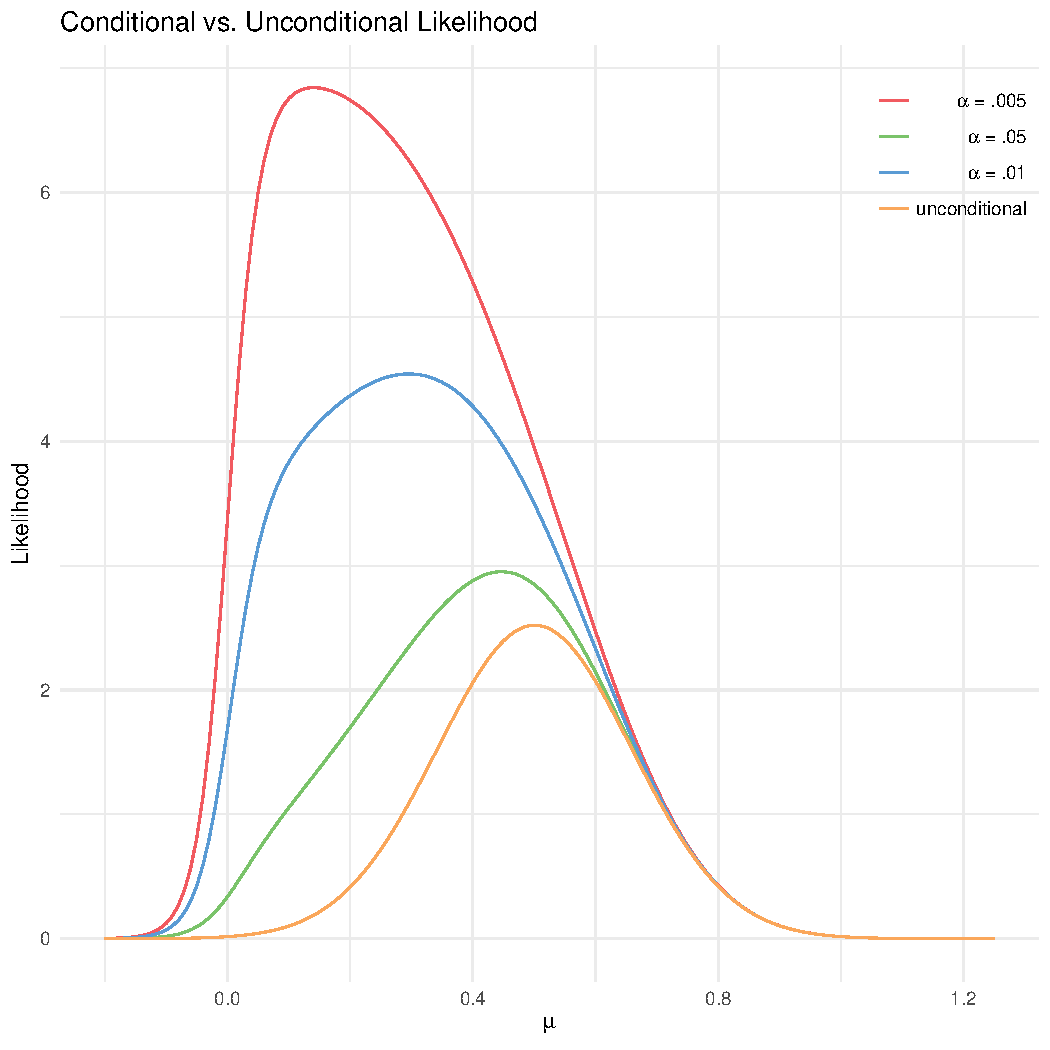
\includegraphics{thesis_files/figure-latex/unnamed-chunk-5-1.pdf}
\begin{Shaded}
\begin{Highlighting}[]
\KeywordTok{kable}\NormalTok{(}\KeywordTok{c}\NormalTok{(}\DataTypeTok{bayes =} \KeywordTok{sqrt}\NormalTok{(}\KeywordTok{sum}\NormalTok{(estimators}\OperatorTok{$}\NormalTok{bayes}\OperatorTok{^}\DecValTok{2}\NormalTok{)), }\DataTypeTok{bayes.median=} \KeywordTok{sqrt}\NormalTok{(}\KeywordTok{sum}\NormalTok{(estimators}\OperatorTok{$}\NormalTok{bayes.median}\OperatorTok{^}\DecValTok{2}\NormalTok{)), }\DataTypeTok{bayes.mode =} \KeywordTok{sqrt}\NormalTok{(}\KeywordTok{sum}\NormalTok{(estimators}\OperatorTok{$}\NormalTok{bayes.mode}\OperatorTok{^}\DecValTok{2}\NormalTok{)),}\DataTypeTok{cond.mean =} \KeywordTok{sqrt}\NormalTok{(}\KeywordTok{sum}\NormalTok{(estimators}\OperatorTok{$}\NormalTok{cond.mean}\OperatorTok{^}\DecValTok{2}\NormalTok{)), }\DataTypeTok{cond.mode =} \KeywordTok{sqrt}\NormalTok{(}\KeywordTok{sum}\NormalTok{(estimators}\OperatorTok{$}\NormalTok{cond.mode}\OperatorTok{^}\DecValTok{2}\NormalTok{)), }\DataTypeTok{naive=} \KeywordTok{sqrt}\NormalTok{(}\KeywordTok{sum}\NormalTok{(estimators}\OperatorTok{$}\NormalTok{naive}\OperatorTok{^}\DecValTok{2}\NormalTok{))), }\DataTypeTok{col.names =} \StringTok{"RMSE"}\NormalTok{)}
\end{Highlighting}
\end{Shaded}
\begin{tabular}{l|r}
\hline
  & RMSE\\
\hline
bayes & 3.827613\\
\hline
bayes.median & 4.365067\\
\hline
bayes.mode & 4.365067\\
\hline
cond.mean & 3.938311\\
\hline
cond.mode & 3.943529\\
\hline
naive & 4.971864\\
\hline
\end{tabular}
The conditional likelihood mode (i.e.~MLE) has the smallest bias
(absolute error) for \(\mu\) out of the frequentist estimators, while
the bayesian median and mode (which end up being the same) the smallest
bias in the bayesian framework. The RMSE for the bayesian estimator
(mean of the posterior) is the lowest, followed by the conditional mean
and mode.

\subsubsection{Credible and Confidence
Intervals}\label{credible-and-confidence-intervals}
\begin{Shaded}
\begin{Highlighting}[]
\NormalTok{##plot of credible interval sizes}
\KeywordTok{ggplot}\NormalTok{(}\DataTypeTok{data =}\NormalTok{ results)}\OperatorTok{+}\StringTok{ }\KeywordTok{geom_point}\NormalTok{(}\KeywordTok{aes}\NormalTok{(}\DataTypeTok{x =}\NormalTok{ conf.upper}\OperatorTok{-}\NormalTok{conf.lower, }\DataTypeTok{y =}\NormalTok{ cred.upper}\OperatorTok{-}\NormalTok{cred.lower, }\DataTypeTok{colour =} \KeywordTok{abs}\NormalTok{(Ybar)))}\OperatorTok{+}\KeywordTok{geom_abline}\NormalTok{(}\DataTypeTok{intercept =} \DecValTok{0}\NormalTok{, }\DataTypeTok{slope =} \DecValTok{1}\NormalTok{)}\OperatorTok{+}\KeywordTok{geom_hline}\NormalTok{(}\DataTypeTok{yintercept=}\DecValTok{2}\OperatorTok{*}\FloatTok{1.96}\OperatorTok{*}\KeywordTok{sqrt}\NormalTok{(}\DecValTok{1}\OperatorTok{/}\DecValTok{100}\NormalTok{))}\OperatorTok{+}\KeywordTok{geom_vline}\NormalTok{(}\DataTypeTok{xintercept=}\DecValTok{2}\OperatorTok{*}\FloatTok{1.96}\OperatorTok{*}\KeywordTok{sqrt}\NormalTok{(}\DecValTok{1}\OperatorTok{/}\DecValTok{100}\NormalTok{))}\OperatorTok{+}\KeywordTok{labs}\NormalTok{(}\DataTypeTok{x=}\StringTok{"Length of (Conditional) Confidence Interval"}\NormalTok{,}\DataTypeTok{y=}\StringTok{"Length of (Bayesian) Credible Interval"}\NormalTok{, }\DataTypeTok{title=}\StringTok{"Interval Size Comparison"}\NormalTok{,}\DataTypeTok{color=}\StringTok{"|Ybar|"}\NormalTok{)}
\end{Highlighting}
\end{Shaded}
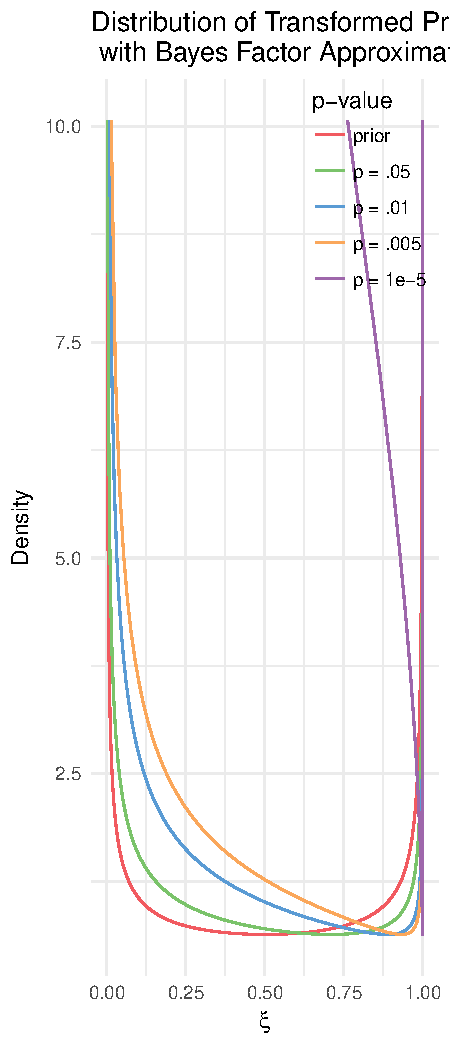
\includegraphics{thesis_files/figure-latex/unnamed-chunk-6-1.pdf}

The lines mark the \(y = x\) line, and the length of naive confidence
intervals (which are constant for fixed number of samples) on the x and
y axes.

The largest values for the significant statistic also correspond to the
largest intervals in both cases. Note that the conditional likelihood
confidence intervals are almost always larger than the credible
intervals, but still mostly smaller than the naive ones.

\subsubsection{Coverage}\label{coverage}

The marginal coverage of the (frequentist conditional likelihood)
confidence interval C,
\(P(\mu \in C|Y) = P(\mu \in C|H_0) P(H_0|Y)+P(\mu \in C|H_1) P(H_1|Y)\)
will be significantly higher than .95 for the cases in which
\(0 \in C\), since \(P(\mu \in C|H_1) =0.95\) by definition, and
\(P(\mu \in C|H_0) = I_{0 \in C}\). In this experiment, the expected
coverage is \(0.98\) for intervals with 0, and only \(0.38\) for those
that do not contain 0.

However, conditioning on the alternative hypothesis does not lead to an
empirical coverage of 95\%.

We can see that both methods are still significantly better than the
naive one.
\begin{Shaded}
\begin{Highlighting}[]
\CommentTok{#table of expected vs empirical coverage}

\NormalTok{results <-}\StringTok{ }\KeywordTok{na.omit}\NormalTok{(results)}
\NormalTok{b <-}\StringTok{ }\KeywordTok{which}\NormalTok{(results}\OperatorTok{$}\NormalTok{H}\OperatorTok{==}\DecValTok{0}\NormalTok{)}

\KeywordTok{kable}\NormalTok{(}\KeywordTok{t}\NormalTok{(}\KeywordTok{data.frame}\NormalTok{(}\DataTypeTok{naive =} \KeywordTok{c}\NormalTok{(}\KeywordTok{mean}\NormalTok{(results}\OperatorTok{$}\NormalTok{naive.cov),}\KeywordTok{mean}\NormalTok{(results[b,]}\OperatorTok{$}\NormalTok{naive.cov),}\KeywordTok{mean}\NormalTok{(results[}\OperatorTok{-}\NormalTok{b,]}\OperatorTok{$}\NormalTok{naive.cov)), }
        \DataTypeTok{conditional =} \KeywordTok{c}\NormalTok{(}\KeywordTok{mean}\NormalTok{(results}\OperatorTok{$}\NormalTok{freq.cov), }\KeywordTok{mean}\NormalTok{(results[b,]}\OperatorTok{$}\NormalTok{freq.cov), }\KeywordTok{mean}\NormalTok{(results[}\OperatorTok{-}\NormalTok{b,]}\OperatorTok{$}\NormalTok{freq.cov)),}
        \DataTypeTok{bayesian =} \KeywordTok{c}\NormalTok{(}\KeywordTok{mean}\NormalTok{(results}\OperatorTok{$}\NormalTok{bayes.cov), }\KeywordTok{mean}\NormalTok{(results[b,]}\OperatorTok{$}\NormalTok{bayes.cov), }\KeywordTok{mean}\NormalTok{(results[}\OperatorTok{-}\NormalTok{b,]}\OperatorTok{$}\NormalTok{bayes.cov)))),}
      \DataTypeTok{col.names =} \KeywordTok{c}\NormalTok{(}\StringTok{"Unconditional Coverage"}\NormalTok{,}\StringTok{"Coverage Conditional on H0"}\NormalTok{, }\StringTok{"Coverage Conditional on H1"}\NormalTok{), }
      \DataTypeTok{row.names =} \OtherTok{TRUE}\NormalTok{,}
      \DataTypeTok{caption =} \StringTok{"Empirical Coverage for 95% Confidence/Credible Intervals"}\NormalTok{)}
\end{Highlighting}
\end{Shaded}
\textbackslash{}begin\{table\}

\textbackslash{}caption\{\label{tab:unnamed-chunk-7}Empirical Coverage for
95\% Confidence/Credible Intervals\} \centering
\begin{tabular}[t]{l|r|r|r}
\hline
  & Unconditional Coverage & Coverage Conditional on H0 & Coverage Conditional on H1\\
\hline
naive & 0.6212766 & 0.5911824 & 0.6941748\\
\hline
conditional & 0.8765957 & 1.0000000 & 0.5776699\\
\hline
bayesian & 0.8765957 & 1.0000000 & 0.5776699\\
\hline
\end{tabular}
\textbackslash{}end\{table\}
\begin{Shaded}
\begin{Highlighting}[]
\CommentTok{#kable(c(naive = , conditional = ,bayesian = mean(results[b,]$bayes.cov)), col.names = c("Empirical Coverage"), caption = "coverage for 95% confidence/credible intervals conditional on H0")}
\CommentTok{#kable(c(naive =c(0) , conditional = mean(results[-b,]$freq.cov),bayesian = mean(results[-b,]$bayes.cov)), col.names = c("Empirical Coverage"), caption = "coverage for 95% confidence/credible intervals conditional on H1")}
\end{Highlighting}
\end{Shaded}
\subsubsection{Hypothesis Rejection(??)}\label{hypothesis-rejection}

Due to the nature of p-values, an \(\alpha = 0.05\) corresponds to a
posterior probability \(P(H_1 | Y )\) of only \(0.4\) for \(N = 100\).
This means that the 95\% credible interval for \(\mu| Y\) will contain 0
every time. In terms of hypothesis testing, if we consider the strategy
of rejecting the null when the interval does not contain 0, this level
for \(\alpha\) leads to no rejections.
\begin{Shaded}
\begin{Highlighting}[]
\NormalTok{##confusion matrices}
\KeywordTok{kable}\NormalTok{(}\KeywordTok{table}\NormalTok{(results}\OperatorTok{$}\NormalTok{H,}\KeywordTok{abs}\NormalTok{(results}\OperatorTok{$}\NormalTok{Ybar)}\OperatorTok{/}\KeywordTok{sqrt}\NormalTok{(}\DecValTok{1}\OperatorTok{/}\DecValTok{100}\NormalTok{)}\OperatorTok{<}\KeywordTok{qnorm}\NormalTok{(}\DecValTok{1}\OperatorTok{-}\FloatTok{0.05}\OperatorTok{/}\DecValTok{2}\NormalTok{))}\OperatorTok{/}\KeywordTok{dim}\NormalTok{(results)[}\DecValTok{1}\NormalTok{], }\DataTypeTok{col.names =} \KeywordTok{c}\NormalTok{(}\StringTok{"Do not reject null"}\NormalTok{, }\StringTok{"Reject null"}\NormalTok{), }\DataTypeTok{row.names =} \OtherTok{TRUE}\NormalTok{, }\DataTypeTok{caption =} \StringTok{"Naive method"}\NormalTok{)}
\end{Highlighting}
\end{Shaded}
\begin{table}

\caption{\label{tab:unnamed-chunk-8}Naive method}
\centering
\begin{tabular}[t]{l|r|r}
\hline
  & Do not reject null & Reject null\\
\hline
0 & 0.2893617 & 0.4184397\\
\hline
1 & 0.1588652 & 0.1333333\\
\hline
\end{tabular}
\end{table}
\begin{Shaded}
\begin{Highlighting}[]
\KeywordTok{kable}\NormalTok{(}\KeywordTok{table}\NormalTok{(results}\OperatorTok{$}\NormalTok{H,results}\OperatorTok{$}\NormalTok{conf.upper}\OperatorTok{>=}\DecValTok{0}\OperatorTok{&}\NormalTok{results}\OperatorTok{$}\NormalTok{conf.lower}\OperatorTok{<=}\DecValTok{0}\NormalTok{)}\OperatorTok{/}\KeywordTok{dim}\NormalTok{(results)[}\DecValTok{1}\NormalTok{], }\DataTypeTok{col.names =} \KeywordTok{c}\NormalTok{(}\StringTok{"Do not reject null"}\NormalTok{), }\DataTypeTok{row.names =} \OtherTok{TRUE}\NormalTok{, }\DataTypeTok{caption =} \StringTok{"Conditional Likelihood Method"}\NormalTok{)}
\end{Highlighting}
\end{Shaded}
\begin{table}

\caption{\label{tab:unnamed-chunk-8}Conditional Likelihood Method}
\centering
\begin{tabular}[t]{l|r}
\hline
  & Do not reject null\\
\hline
0 & 0.7078014\\
\hline
1 & 0.2921986\\
\hline
\end{tabular}
\end{table}
\begin{Shaded}
\begin{Highlighting}[]
\KeywordTok{kable}\NormalTok{(}\KeywordTok{table}\NormalTok{(results}\OperatorTok{$}\NormalTok{H,results}\OperatorTok{$}\NormalTok{cred.upper}\OperatorTok{>=}\DecValTok{0}\OperatorTok{&}\NormalTok{results}\OperatorTok{$}\NormalTok{cred.lower}\OperatorTok{<=}\DecValTok{0}\NormalTok{)}\OperatorTok{/}\KeywordTok{dim}\NormalTok{(results)[}\DecValTok{1}\NormalTok{], }\DataTypeTok{col.names =} \KeywordTok{c}\NormalTok{(}\StringTok{"Do not reject null"}\NormalTok{), }\DataTypeTok{row.names =} \OtherTok{TRUE}\NormalTok{, }\DataTypeTok{caption =} \StringTok{"Bayesian Mixture Model"}\NormalTok{)}
\end{Highlighting}
\end{Shaded}
\begin{table}

\caption{\label{tab:unnamed-chunk-8}Bayesian Mixture Model}
\centering
\begin{tabular}[t]{l|r}
\hline
  & Do not reject null\\
\hline
0 & 0.7078014\\
\hline
1 & 0.2921986\\
\hline
\end{tabular}
\end{table}
Despite never rejecting the null, the conditional likelihood and the
bayesian methods both perform better than the naive one in terms of
``predicting'' accurately. The naive method is especially problematic in
that it has a higher Type 1 error (false positives) than true positives
OR true negatives in the region of the data.

\textbf{\#\# Double Exponential Simulation with Adjusted P-Values}

\chapter{Hierarchical Model
Simulation}\label{hierarchical-model-simulation}

This simulation generates data from a hierarchical logistic model as
follows: If there is a true association, \(\mu\) is a (fixed) nonzero
value and \(\beta_j \sim N(\mu, \sigma^2)\) where \(\sigma^2\) is fixed.
Otherwise, \(\mu=\beta_j = 0, \forall j\). The observed data \(Y_{ij}\)
is binary, and has
\(P(Y_{ij}| \beta_j) = \frac{e^{\beta_j}}{1+e^{\beta_j}}\). The \(j\)
index corresponds to the ``group'' to which the observation belongs.
\begin{Shaded}
\begin{Highlighting}[]
\NormalTok{knitr}\OperatorTok{::}\NormalTok{opts_chunk}\OperatorTok{$}\KeywordTok{set}\NormalTok{(}\DataTypeTok{echo =} \OtherTok{TRUE}\NormalTok{)}
\NormalTok{knitr}\OperatorTok{::}\NormalTok{opts_chunk}\OperatorTok{$}\KeywordTok{set}\NormalTok{(}\DataTypeTok{cache =} \OtherTok{TRUE}\NormalTok{)}
\KeywordTok{library}\NormalTok{(}\StringTok{"R2jags"}\NormalTok{)}
\end{Highlighting}
\end{Shaded}
\begin{verbatim}
Loading required package: rjags
\end{verbatim}
\begin{verbatim}
Loading required package: coda
\end{verbatim}
\begin{verbatim}
Linked to JAGS 4.2.0
\end{verbatim}
\begin{verbatim}
Loaded modules: basemod,bugs
\end{verbatim}
\begin{verbatim}

Attaching package: 'R2jags'
\end{verbatim}
\begin{verbatim}
The following object is masked from 'package:coda':

    traceplot
\end{verbatim}
\begin{Shaded}
\begin{Highlighting}[]
\KeywordTok{set.seed}\NormalTok{(}\DecValTok{1}\NormalTok{)}
\NormalTok{epsilon=.}\DecValTok{01}
\CommentTok{#fix everything (even betas)}
\NormalTok{mu.p53=.}\DecValTok{5}
\NormalTok{phi.p53=}\StringTok{ }\DecValTok{10}
\NormalTok{observations=}\DecValTok{1000}
\NormalTok{n.sites=}\DecValTok{7}
\NormalTok{beta.p53.fixed =}\StringTok{ }\KeywordTok{rnorm}\NormalTok{(n.sites,mu.p53,phi.p53}\OperatorTok{^}\NormalTok{(}\OperatorTok{-}\NormalTok{.}\DecValTok{5}\NormalTok{)) }\CommentTok{#"fixed" because seed}
\NormalTok{beta.p53.fixed.}\DecValTok{1}\NormalTok{ <-beta.p53.fixed}
\NormalTok{Y <-site <-}\StringTok{ }\KeywordTok{rep}\NormalTok{(}\OtherTok{NA}\NormalTok{, observations}\OperatorTok{*}\NormalTok{n.sites)}
\ControlFlowTok{for}\NormalTok{(i }\ControlFlowTok{in} \DecValTok{1}\OperatorTok{:}\NormalTok{n.sites)\{}
\NormalTok{    Y[((i}\OperatorTok{-}\DecValTok{1}\NormalTok{)}\OperatorTok{*}\NormalTok{observations}\OperatorTok{+}\DecValTok{1}\NormalTok{)}\OperatorTok{:}\NormalTok{(i}\OperatorTok{*}\NormalTok{observations)]<-}\KeywordTok{rbinom}\NormalTok{(observations, }\DecValTok{1}\NormalTok{, }\KeywordTok{exp}\NormalTok{(beta.p53.fixed[i])}\OperatorTok{/}\NormalTok{(}\DecValTok{1}\OperatorTok{+}\KeywordTok{exp}\NormalTok{(beta.p53.fixed[i])))}
\NormalTok{    site[((i}\OperatorTok{-}\DecValTok{1}\NormalTok{)}\OperatorTok{*}\NormalTok{observations}\OperatorTok{+}\DecValTok{1}\NormalTok{)}\OperatorTok{:}\NormalTok{(i}\OperatorTok{*}\NormalTok{observations)]<-}\StringTok{ }\KeywordTok{rep}\NormalTok{(i, observations)}
\NormalTok{\}}
\NormalTok{sim.data1.}\DecValTok{1}\NormalTok{<-}\KeywordTok{list}\NormalTok{(}\DataTypeTok{CaseCon=}\NormalTok{Y, }\DataTypeTok{site=}\NormalTok{site,  }\DataTypeTok{J=}\NormalTok{n.sites}\OperatorTok{*}\NormalTok{observations ,}\DataTypeTok{n.sites=}\NormalTok{n.sites)}

\NormalTok{Y <-site <-}\StringTok{ }\KeywordTok{rep}\NormalTok{(}\OtherTok{NA}\NormalTok{, observations}\OperatorTok{*}\NormalTok{n.sites)}
\ControlFlowTok{for}\NormalTok{(i }\ControlFlowTok{in} \DecValTok{1}\OperatorTok{:}\NormalTok{n.sites)\{}
\NormalTok{  Y[((i}\OperatorTok{-}\DecValTok{1}\NormalTok{)}\OperatorTok{*}\NormalTok{observations}\OperatorTok{+}\DecValTok{1}\NormalTok{)}\OperatorTok{:}\NormalTok{(i}\OperatorTok{*}\NormalTok{observations)]<-}\KeywordTok{rbinom}\NormalTok{(observations, }\DecValTok{1}\NormalTok{,.}\DecValTok{5}\NormalTok{) }\CommentTok{#beta=0}
\NormalTok{  site[((i}\OperatorTok{-}\DecValTok{1}\NormalTok{)}\OperatorTok{*}\NormalTok{observations}\OperatorTok{+}\DecValTok{1}\NormalTok{)}\OperatorTok{:}\NormalTok{(i}\OperatorTok{*}\NormalTok{observations)]<-}\StringTok{ }\KeywordTok{rep}\NormalTok{(i, observations)}
\NormalTok{\}}
\NormalTok{sim.data1.}\DecValTok{0}\NormalTok{<-}\KeywordTok{list}\NormalTok{(}\DataTypeTok{CaseCon=}\NormalTok{Y, }\DataTypeTok{site=}\NormalTok{site,  }\DataTypeTok{J=}\NormalTok{n.sites}\OperatorTok{*}\NormalTok{observations ,}\DataTypeTok{n.sites=}\NormalTok{n.sites)}
\CommentTok{#this might just be 0?}

\KeywordTok{set.seed}\NormalTok{(}\DecValTok{1}\NormalTok{)}
\NormalTok{mu.p53=.}\DecValTok{1}
\NormalTok{phi.p53=}\StringTok{ }\DecValTok{10}
\NormalTok{observations=}\DecValTok{100}
\NormalTok{n.sites=}\DecValTok{7}
\NormalTok{beta.p53.fixed =}\StringTok{ }\KeywordTok{rnorm}\NormalTok{(n.sites,mu.p53,phi.p53}\OperatorTok{^}\NormalTok{(}\OperatorTok{-}\NormalTok{.}\DecValTok{5}\NormalTok{)) }\CommentTok{#"fixed" because seed}
\NormalTok{beta.p53.fixed.}\DecValTok{2}\NormalTok{ <-beta.p53.fixed}
\NormalTok{Y <-site <-}\StringTok{ }\KeywordTok{rep}\NormalTok{(}\OtherTok{NA}\NormalTok{, observations}\OperatorTok{*}\NormalTok{n.sites)}
\ControlFlowTok{for}\NormalTok{(i }\ControlFlowTok{in} \DecValTok{1}\OperatorTok{:}\NormalTok{n.sites)\{}
\NormalTok{    Y[((i}\OperatorTok{-}\DecValTok{1}\NormalTok{)}\OperatorTok{*}\NormalTok{observations}\OperatorTok{+}\DecValTok{1}\NormalTok{)}\OperatorTok{:}\NormalTok{(i}\OperatorTok{*}\NormalTok{observations)]<-}\KeywordTok{rbinom}\NormalTok{(observations, }\DecValTok{1}\NormalTok{, }\KeywordTok{exp}\NormalTok{(beta.p53.fixed[i])}\OperatorTok{/}\NormalTok{(}\DecValTok{1}\OperatorTok{+}\KeywordTok{exp}\NormalTok{(beta.p53.fixed[i])))}
\NormalTok{    site[((i}\OperatorTok{-}\DecValTok{1}\NormalTok{)}\OperatorTok{*}\NormalTok{observations}\OperatorTok{+}\DecValTok{1}\NormalTok{)}\OperatorTok{:}\NormalTok{(i}\OperatorTok{*}\NormalTok{observations)]<-}\StringTok{ }\KeywordTok{rep}\NormalTok{(i, observations)}
\NormalTok{\}}
\NormalTok{sim.data1.}\DecValTok{2}\NormalTok{<-}\KeywordTok{list}\NormalTok{(}\DataTypeTok{CaseCon=}\NormalTok{Y, }\DataTypeTok{site=}\NormalTok{site,  }\DataTypeTok{J=}\NormalTok{n.sites}\OperatorTok{*}\NormalTok{observations ,}\DataTypeTok{n.sites=}\NormalTok{n.sites)}

\KeywordTok{source}\NormalTok{(}\StringTok{"HPD.R"}\NormalTok{)}
\NormalTok{#############}
\end{Highlighting}
\end{Shaded}
Since there is uncertainty regarding whether or not there is a true
association, this can be modeled as a probability \(\xi\) with a beta
prior. Then an inverse gamma prior is chosen for variance \(\sigma^2\)
and a spike and slab prior conditioning on the probability of
association for \(mu\):
\(\pi(\mu|\xi) = (1-\xi ) \delta_0(\mu)+ \xi\phi(\mu)\).

There are a couple of changes that can be made in the model
implementation to to obtain MCMC samples:
\begin{enumerate}
\def\labelenumi{\arabic{enumi}.}
\item
  The point mass can be approximated using a very concentrated normal
  distribution, centered at 0. Thus,
  \(\pi(\mu|\xi) = (1-\xi) N(\mu, 0, \epsilon)+ \xi N(\mu,0 ,1)\).
\item
  The probability \(\xi\) can give rise to a latent variable drawn from
  a bernoulli, which is then used to parametrize the distribution of
  \(\mu\). That is,
  \(\pi(\mu|\iota) = (1-\iota ) N(\mu, 0, \epsilon)+ \iota N(\mu,0 ,1)\),
  and \(P(\iota = 1 ) = \xi\).
\end{enumerate}
However, due to the sequential nature of MCMC sampling, these seemingly
identical models produce different results.

Models that do not use the latent variable must specify the mixture
distribution in JAGS directly. This is done through the zeroes and ones
trick, which use properties of the Poisson and Bernoulli distributions
in order to allow for arbitrary distributions.

In these scenarios, the model from which a sample comes from is also not
evident. To determine whether a small value is truly from the
concentrated normal, we can compute the probability of the sample for
the two distributions and choose the model that results in a larger one.

\emph{not sure how relevant this is, maybe will remove different
implementations once things work out}
\begin{Shaded}
\begin{Highlighting}[]
\CommentTok{#model}
\NormalTok{p53.test.ind =}\StringTok{ }\ControlFlowTok{function}\NormalTok{() \{}
  \ControlFlowTok{for}\NormalTok{ (j }\ControlFlowTok{in} \DecValTok{1}\OperatorTok{:}\NormalTok{J) \{}
\NormalTok{    CaseCon[j] }\OperatorTok{~}\StringTok{ }\KeywordTok{dbern}\NormalTok{(theta[j])}
    \KeywordTok{logit}\NormalTok{(theta[j]) <-}\StringTok{  }\NormalTok{beta.p53[site[j]]  \}}
  
  \ControlFlowTok{for}\NormalTok{ (l }\ControlFlowTok{in} \DecValTok{1}\OperatorTok{:}\NormalTok{n.sites) \{}
\NormalTok{    beta.p53.}\DecValTok{1}\NormalTok{[l] }\OperatorTok{~}\StringTok{ }\KeywordTok{dnorm}\NormalTok{(mu.p53, phi.p53)}
\NormalTok{    beta.p53[l] <-}\StringTok{ }\NormalTok{beta.p53.}\DecValTok{1}\NormalTok{[l]}\OperatorTok{*}\NormalTok{(mu.p53.notzero)}
\NormalTok{  \}}
  \CommentTok{#zeroes trick}
\NormalTok{  C<-}\DecValTok{1000}
\NormalTok{  epsilon<-}\FloatTok{0.01}
\NormalTok{  tau<-}\StringTok{ }\KeywordTok{pow}\NormalTok{(epsilon,}\OperatorTok{-}\DecValTok{2}\NormalTok{)}
  \CommentTok{#if mu geq 0 and mu leq 0, prior is from point mass}
  \CommentTok{#mu in (-epsilon, epsilon)}
\NormalTok{  mu.p53.notzero<-}\StringTok{ }\KeywordTok{step}\NormalTok{(}\KeywordTok{abs}\NormalTok{(mu.p53)}\OperatorTok{-}\NormalTok{epsilon) }\CommentTok{#LR and then decide}
\NormalTok{  L<-}\StringTok{ }\NormalTok{(}\DecValTok{1}\OperatorTok{-}\NormalTok{mu.p53.notzero)}\OperatorTok{*}\NormalTok{(}\DecValTok{1}\OperatorTok{-}\NormalTok{pind)}\OperatorTok{+}\StringTok{ }\CommentTok{#(dnorm(mu.p53,0,tau)*(1-pind))+ #}
\StringTok{    }\NormalTok{(}\KeywordTok{dnorm}\NormalTok{(mu.p53,}\DecValTok{0}\NormalTok{,}\DecValTok{1}\NormalTok{)}\OperatorTok{*}\NormalTok{pind)}
  \CommentTok{#need pind for mixing}
  
\NormalTok{  phi<-}\StringTok{ }\OperatorTok{-}\KeywordTok{log}\NormalTok{(L)}\OperatorTok{+}\NormalTok{C}
\NormalTok{  zero}\OperatorTok{~}\KeywordTok{dpois}\NormalTok{(phi)}
\NormalTok{  mu.p53 }\OperatorTok{~}\StringTok{ }\KeywordTok{dunif}\NormalTok{(}\OperatorTok{-}\DecValTok{10}\NormalTok{,}\DecValTok{10}\NormalTok{) }\CommentTok{#not sure how big this interval should be, just picked one large enough for .1 sd, started at 10, but even 1 has too large jumps}
  
\NormalTok{  phi.p53 }\OperatorTok{~}\StringTok{ }\KeywordTok{dgamma}\NormalTok{(}\DecValTok{1}\NormalTok{, .}\DecValTok{05}\NormalTok{)}
  \CommentTok{#    phi.p53 ~ dgamma(2, .02)}
\NormalTok{  sigma.p53 <-}\StringTok{ }\KeywordTok{pow}\NormalTok{(phi.p53, }\OperatorTok{-}\NormalTok{.}\DecValTok{5}\NormalTok{)}
  
  \CommentTok{#assoc~dbern(pind)}
\NormalTok{  pind }\OperatorTok{~}\StringTok{ }\KeywordTok{dbeta}\NormalTok{(.}\DecValTok{5}\NormalTok{,.}\DecValTok{5}\NormalTok{)}
\NormalTok{\}}


\NormalTok{p53.test.approx=}\StringTok{ }\ControlFlowTok{function}\NormalTok{() \{}
  \ControlFlowTok{for}\NormalTok{ (j }\ControlFlowTok{in} \DecValTok{1}\OperatorTok{:}\NormalTok{J) \{}
\NormalTok{    CaseCon[j] }\OperatorTok{~}\StringTok{ }\KeywordTok{dbern}\NormalTok{(theta[j])}
    \KeywordTok{logit}\NormalTok{(theta[j]) <-}\StringTok{  }\NormalTok{beta.p53[site[j]]  \}}
  
  \ControlFlowTok{for}\NormalTok{ (l }\ControlFlowTok{in} \DecValTok{1}\OperatorTok{:}\NormalTok{n.sites) \{}
\NormalTok{    beta.p53.}\DecValTok{1}\NormalTok{[l] }\OperatorTok{~}\StringTok{ }\KeywordTok{dnorm}\NormalTok{(mu.p53, phi.p53)}
\NormalTok{    beta.p53[l] <-}\StringTok{ }\NormalTok{beta.p53.}\DecValTok{1}\NormalTok{[l]}\OperatorTok{*}\NormalTok{(mu.p53.notzero)}
\NormalTok{  \}}
  \CommentTok{#zeroes trick}
\NormalTok{  C<-}\DecValTok{1000}
\NormalTok{  epsilon<-}\FloatTok{0.01}
\NormalTok{  tau<-}\StringTok{ }\KeywordTok{pow}\NormalTok{(epsilon,}\OperatorTok{-}\DecValTok{2}\NormalTok{)}
  \CommentTok{#if mu geq 0 and mu leq 0, prior is from point mass}
  \CommentTok{#is not zero if prob is greater}
\NormalTok{  mu.p53.notzero<-}\StringTok{ }\KeywordTok{step}\NormalTok{(temp) }\CommentTok{#should come from this?}
\NormalTok{  temp<-}\KeywordTok{dnorm}\NormalTok{(mu.p53,}\DecValTok{0}\NormalTok{,}\DecValTok{1}\NormalTok{)}\OperatorTok{-}\KeywordTok{dnorm}\NormalTok{(mu.p53,}\DecValTok{0}\NormalTok{,tau)}
\NormalTok{  L<-}\StringTok{ }\NormalTok{(}\KeywordTok{dnorm}\NormalTok{(mu.p53,}\DecValTok{0}\NormalTok{,tau)}\OperatorTok{*}\NormalTok{(}\DecValTok{1}\OperatorTok{-}\NormalTok{pind))}\OperatorTok{+}\StringTok{ }\CommentTok{#(1- mu.p53.notzero)*(1-pind)+ #}
\StringTok{    }\NormalTok{(}\KeywordTok{dnorm}\NormalTok{(mu.p53,}\DecValTok{0}\NormalTok{,}\DecValTok{1}\NormalTok{)}\OperatorTok{*}\NormalTok{pind)}
  \CommentTok{#need pind for mixing}
  
\NormalTok{  phi<-}\StringTok{ }\OperatorTok{-}\KeywordTok{log}\NormalTok{(L)}\OperatorTok{+}\NormalTok{C}
\NormalTok{  zero}\OperatorTok{~}\KeywordTok{dpois}\NormalTok{(phi)}
\NormalTok{  mu.p53 }\OperatorTok{~}\StringTok{ }\KeywordTok{dunif}\NormalTok{(}\OperatorTok{-}\DecValTok{10}\NormalTok{,}\DecValTok{10}\NormalTok{) }\CommentTok{#not sure how big this interval should be, just picked one large enough for .1 sd, started at 10, but even 1 has too large jumps}
  
\NormalTok{  phi.p53 }\OperatorTok{~}\StringTok{ }\KeywordTok{dgamma}\NormalTok{(}\DecValTok{1}\NormalTok{, .}\DecValTok{05}\NormalTok{)}
  \CommentTok{#    phi.p53 ~ dgamma(2, .02)}
\NormalTok{  sigma.p53 <-}\StringTok{ }\KeywordTok{pow}\NormalTok{(phi.p53, }\OperatorTok{-}\NormalTok{.}\DecValTok{5}\NormalTok{)}
  
  \CommentTok{#assoc~dbern(pind)}
\NormalTok{  pind }\OperatorTok{~}\StringTok{ }\KeywordTok{dbeta}\NormalTok{(.}\DecValTok{5}\NormalTok{,.}\DecValTok{5}\NormalTok{)}
\NormalTok{\}}


\NormalTok{p53.test.latent=}\StringTok{ }\ControlFlowTok{function}\NormalTok{() \{}
  \ControlFlowTok{for}\NormalTok{ (j }\ControlFlowTok{in} \DecValTok{1}\OperatorTok{:}\NormalTok{J) \{}
\NormalTok{    CaseCon[j] }\OperatorTok{~}\StringTok{ }\KeywordTok{dbern}\NormalTok{(theta[j])}
    \KeywordTok{logit}\NormalTok{(theta[j]) <-}\StringTok{  }\NormalTok{beta.p53[site[j]]  \}}
  
  \ControlFlowTok{for}\NormalTok{ (l }\ControlFlowTok{in} \DecValTok{1}\OperatorTok{:}\NormalTok{n.sites) \{}
\NormalTok{    beta.p53.}\DecValTok{1}\NormalTok{[l] }\OperatorTok{~}\StringTok{ }\KeywordTok{dnorm}\NormalTok{(mu.p53, phi.p53)}
\NormalTok{    beta.p53[l] <-}\StringTok{ }\NormalTok{beta.p53.}\DecValTok{1}\NormalTok{[l]}\OperatorTok{*}\NormalTok{(mu.p53.notzero)}
\NormalTok{  \}}
  \CommentTok{#zeroes trick}
\NormalTok{  C<-}\DecValTok{1000}
\NormalTok{  epsilon<-}\FloatTok{0.01}
\NormalTok{  tau<-}\StringTok{ }\KeywordTok{pow}\NormalTok{(epsilon,}\OperatorTok{-}\DecValTok{2}\NormalTok{)}
  \CommentTok{#if mu geq 0 and mu leq 0, prior is from point mass}
  \CommentTok{#is not zero if prob is greater}
\NormalTok{  mu.p53.notzero<-}\StringTok{ }\NormalTok{assoc}
\NormalTok{  temp<-}\KeywordTok{dnorm}\NormalTok{(mu.p53,}\DecValTok{0}\NormalTok{,}\DecValTok{1}\NormalTok{)}\OperatorTok{-}\KeywordTok{dnorm}\NormalTok{(mu.p53,}\DecValTok{0}\NormalTok{,tau)}
  \CommentTok{#L<- (dnorm(mu.p53,0,tau)^(1-assoc))*(dnorm(mu.p53,0,1)^(assoc))}
  \CommentTok{#need pind for mixing}
  
  \CommentTok{#phi<- -log(L)+C}
  \CommentTok{#zero~dpois(phi)}
  \CommentTok{#mu.p53 ~ dunif(-10,10) #not sure how big this interval should be, just picked one large enough for .1 sd, started at 10, but even 1 has too large jumps}
\NormalTok{  mu.p53<-}\StringTok{ }\NormalTok{mu1.p53}\OperatorTok{*}\NormalTok{assoc}
\NormalTok{  mu1.p53 }\OperatorTok{~}\StringTok{ }\KeywordTok{dnorm}\NormalTok{(}\DecValTok{0}\NormalTok{,}\DecValTok{1}\NormalTok{)}
\NormalTok{  phi.p53 }\OperatorTok{~}\StringTok{ }\KeywordTok{dgamma}\NormalTok{(}\DecValTok{1}\NormalTok{, .}\DecValTok{05}\NormalTok{)}
  \CommentTok{#    phi.p53 ~ dgamma(2, .02)}
\NormalTok{  sigma.p53 <-}\StringTok{ }\KeywordTok{pow}\NormalTok{(phi.p53, }\OperatorTok{-}\NormalTok{.}\DecValTok{5}\NormalTok{)}
  
\NormalTok{  assoc}\OperatorTok{~}\KeywordTok{dbern}\NormalTok{(pind)}
\NormalTok{  pind }\OperatorTok{~}\StringTok{ }\KeywordTok{dbeta}\NormalTok{(.}\DecValTok{5}\NormalTok{,.}\DecValTok{5}\NormalTok{)}
\NormalTok{\}}
\end{Highlighting}
\end{Shaded}
\begin{Shaded}
\begin{Highlighting}[]
\NormalTok{p53.fulljags1.}\FloatTok{0.}\NormalTok{a =}\StringTok{ }\KeywordTok{jags}\NormalTok{(}\DataTypeTok{data=}\NormalTok{sim.data1.}\DecValTok{0}\NormalTok{, ####this}
                    \DataTypeTok{inits=}\OtherTok{NULL}\NormalTok{, }\DataTypeTok{parameters.to.save =}\KeywordTok{c}\NormalTok{(}\StringTok{"pind"}\NormalTok{, }\StringTok{"mu.p53"}\NormalTok{, }\StringTok{"phi.p53"}\NormalTok{,}\StringTok{"mu.p53.notzero"}\NormalTok{,}\StringTok{"temp"}\NormalTok{),}
                    \DataTypeTok{model =}\NormalTok{ p53.test.approx)}
\end{Highlighting}
\end{Shaded}
\begin{verbatim}
module glm loaded
\end{verbatim}
\begin{verbatim}
Compiling model graph
   Resolving undeclared variables
   Allocating nodes
Graph information:
   Observed stochastic nodes: 7000
   Unobserved stochastic nodes: 11
   Total graph size: 14076

Initializing model
\end{verbatim}
\begin{Shaded}
\begin{Highlighting}[]
\CommentTok{#par(mar=rep(1,4))}
\CommentTok{#plot(as.mcmc(p53.fulljags1.0.a))}
\KeywordTok{HPDM}\NormalTok{(p53.fulljags1.}\FloatTok{0.}\NormalTok{a}\OperatorTok{$}\NormalTok{BUGSoutput}\OperatorTok{$}\NormalTok{sims.list}\OperatorTok{$}\NormalTok{mu.p53, }\DataTypeTok{e=}\NormalTok{epsilon)}
\end{Highlighting}
\end{Shaded}
\begin{verbatim}


Potentially multimodal column vectors:
 1 

Column 1 multimodal intervals:  (-0.036,0.041) 
\end{verbatim}
\includegraphics{thesis_files/figure-latex/fixed 0-1.pdf}
\begin{verbatim}
           Lower     Upper
[1,] -0.03566506 0.0405582
\end{verbatim}
\begin{Shaded}
\begin{Highlighting}[]
\KeywordTok{mean}\NormalTok{(p53.fulljags1.}\FloatTok{0.}\NormalTok{a}\OperatorTok{$}\NormalTok{BUGSoutput}\OperatorTok{$}\NormalTok{sims.list}\OperatorTok{$}\NormalTok{mu.p53)}
\end{Highlighting}
\end{Shaded}
\begin{verbatim}
[1] 0.001147017
\end{verbatim}
\begin{Shaded}
\begin{Highlighting}[]
\KeywordTok{median}\NormalTok{(p53.fulljags1.}\FloatTok{0.}\NormalTok{a}\OperatorTok{$}\NormalTok{BUGSoutput}\OperatorTok{$}\NormalTok{sims.list}\OperatorTok{$}\NormalTok{mu.p53)}
\end{Highlighting}
\end{Shaded}
\begin{verbatim}
[1] 0.001183041
\end{verbatim}
\begin{Shaded}
\begin{Highlighting}[]
\NormalTok{p53.fulljags1.}\FloatTok{0.}\NormalTok{i =}\StringTok{ }\KeywordTok{jags}\NormalTok{(}\DataTypeTok{data=}\NormalTok{sim.data1.}\DecValTok{0}\NormalTok{, ####this}
                    \DataTypeTok{inits=}\OtherTok{NULL}\NormalTok{, }\DataTypeTok{parameters.to.save =}\KeywordTok{c}\NormalTok{(}\StringTok{"pind"}\NormalTok{, }\StringTok{"mu.p53"}\NormalTok{, }\StringTok{"phi.p53"}\NormalTok{,}\StringTok{"mu.p53.notzero"}\NormalTok{),}
                    \DataTypeTok{model =}\NormalTok{ p53.test.ind)}
\end{Highlighting}
\end{Shaded}
\begin{verbatim}
Compiling model graph
   Resolving undeclared variables
   Allocating nodes
Graph information:
   Observed stochastic nodes: 7000
   Unobserved stochastic nodes: 11
   Total graph size: 14068

Initializing model
\end{verbatim}
\begin{Shaded}
\begin{Highlighting}[]
\CommentTok{#par(mar=rep(1,4))}
\CommentTok{#plot(as.mcmc(p53.fulljags1.0.i))}
\KeywordTok{HPDM}\NormalTok{(p53.fulljags1.}\FloatTok{0.}\NormalTok{i}\OperatorTok{$}\NormalTok{BUGSoutput}\OperatorTok{$}\NormalTok{sims.list}\OperatorTok{$}\NormalTok{mu.p53, }\DataTypeTok{e=}\NormalTok{epsilon)}
\end{Highlighting}
\end{Shaded}
\begin{verbatim}


Potentially multimodal column vectors:
 1 

Column 1 multimodal intervals:  (-0.08,-0.016) (-0.01,0.01) 
\end{verbatim}
\includegraphics{thesis_files/figure-latex/fixed 0-2.pdf}
\begin{verbatim}
           Lower       Upper                         
[1,] -0.07958173 -0.01596594 -0.009995439 0.009995481
\end{verbatim}
\begin{Shaded}
\begin{Highlighting}[]
\KeywordTok{mean}\NormalTok{(p53.fulljags1.}\FloatTok{0.}\NormalTok{i}\OperatorTok{$}\NormalTok{BUGSoutput}\OperatorTok{$}\NormalTok{sims.list}\OperatorTok{$}\NormalTok{mu.p53)}
\end{Highlighting}
\end{Shaded}
\begin{verbatim}
[1] -0.002581946
\end{verbatim}
\begin{Shaded}
\begin{Highlighting}[]
\KeywordTok{median}\NormalTok{(p53.fulljags1.}\FloatTok{0.}\NormalTok{i}\OperatorTok{$}\NormalTok{BUGSoutput}\OperatorTok{$}\NormalTok{sims.list}\OperatorTok{$}\NormalTok{mu.p53)}
\end{Highlighting}
\end{Shaded}
\begin{verbatim}
[1] -0.0003995983
\end{verbatim}
\begin{Shaded}
\begin{Highlighting}[]
\KeywordTok{plotvar}\NormalTok{(p53.fulljags1.}\FloatTok{0.}\NormalTok{a}\OperatorTok{$}\NormalTok{BUGSoutput}\OperatorTok{$}\NormalTok{sims.list}\OperatorTok{$}\NormalTok{mu.p53,}\DataTypeTok{e=}\NormalTok{epsilon)}
\KeywordTok{plotvar}\NormalTok{(p53.fulljags1.}\FloatTok{0.}\NormalTok{i}\OperatorTok{$}\NormalTok{BUGSoutput}\OperatorTok{$}\NormalTok{sims.list}\OperatorTok{$}\NormalTok{mu.p53,}\DataTypeTok{e=}\NormalTok{epsilon,}\DataTypeTok{newplot=}\OtherTok{FALSE}\NormalTok{)}
\end{Highlighting}
\end{Shaded}
\includegraphics{thesis_files/figure-latex/fixed 0-3.pdf}
\begin{Shaded}
\begin{Highlighting}[]
\CommentTok{#glm}
\NormalTok{p53.fullglm1.}\DecValTok{0}\NormalTok{ =}\StringTok{ }\KeywordTok{glm}\NormalTok{(CaseCon }\OperatorTok{~}\StringTok{ }\KeywordTok{factor}\NormalTok{(site), }\DataTypeTok{data=}\NormalTok{sim.data1.}\DecValTok{0}\NormalTok{,  ####also this}
               \DataTypeTok{family=}\NormalTok{binomial, }\DataTypeTok{x=}\NormalTok{T)}

\KeywordTok{coef}\NormalTok{(p53.fullglm1.}\DecValTok{0}\NormalTok{)}
\end{Highlighting}
\end{Shaded}
\begin{verbatim}
  (Intercept) factor(site)2 factor(site)3 factor(site)4 factor(site)5 
  -0.10810516    0.11210517    0.07610243    0.21219905    0.02405572 
factor(site)6 factor(site)7 
   0.07610243    0.12810583 
\end{verbatim}
\begin{Shaded}
\begin{Highlighting}[]
\KeywordTok{confint}\NormalTok{(p53.fullglm1.}\DecValTok{0}\NormalTok{)}
\end{Highlighting}
\end{Shaded}
\begin{verbatim}
Waiting for profiling to be done...
\end{verbatim}
\begin{verbatim}
                    2.5 %     97.5 %
(Intercept)   -0.23242434 0.01593609
factor(site)2 -0.06328383 0.28763842
factor(site)3 -0.09932072 0.25162370
factor(site)4  0.03675574 0.38791507
factor(site)5 -0.15146721 0.19960978
factor(site)6 -0.09932072 0.25162370
factor(site)7 -0.04727711 0.30365352
\end{verbatim}
\begin{Shaded}
\begin{Highlighting}[]
\NormalTok{p53.fullglm1.}\FloatTok{0.}\NormalTok{simple =}\StringTok{ }\KeywordTok{glm}\NormalTok{(CaseCon }\OperatorTok{~}\StringTok{ }\DecValTok{1}\NormalTok{, }\DataTypeTok{data=}\NormalTok{sim.data1.}\DecValTok{0}\NormalTok{,  ####also this}
               \DataTypeTok{family=}\NormalTok{binomial, }\DataTypeTok{x=}\NormalTok{T)}
\KeywordTok{coef}\NormalTok{(p53.fullglm1.}\FloatTok{0.}\NormalTok{simple)}
\end{Highlighting}
\end{Shaded}
\begin{verbatim}
(Intercept) 
-0.01828622 
\end{verbatim}
Overall the Bayesian and frequentist results on this (nonassociated)
dataset are very similar. Using a parameter vs an index does produce
significantly different results at this stage. Even while using the same
prior for pind, the index-based model has a greater amount of ``0''s.
However, this does not change the posterior of pind (\(\xi\)). On the
other hand, the normal approx at least shifts it towards 0 (which is
what we expect).
\begin{Shaded}
\begin{Highlighting}[]
\NormalTok{p53.fulljags1.}\FloatTok{1.}\NormalTok{a =}\StringTok{ }\KeywordTok{jags}\NormalTok{(}\DataTypeTok{data=}\NormalTok{sim.data1.}\DecValTok{1}\NormalTok{, ####this}
                    \DataTypeTok{inits=}\OtherTok{NULL}\NormalTok{, }\DataTypeTok{parameters.to.save =}\KeywordTok{c}\NormalTok{(}\StringTok{"pind"}\NormalTok{, }\StringTok{"mu.p53"}\NormalTok{, }\StringTok{"phi.p53"}\NormalTok{,}\StringTok{"mu.p53.notzero"}\NormalTok{),}
                    \DataTypeTok{model =}\NormalTok{ p53.test.approx)}
\end{Highlighting}
\end{Shaded}
\begin{verbatim}
Compiling model graph
   Resolving undeclared variables
   Allocating nodes
Graph information:
   Observed stochastic nodes: 7000
   Unobserved stochastic nodes: 11
   Total graph size: 14076

Initializing model
\end{verbatim}
\begin{Shaded}
\begin{Highlighting}[]
\CommentTok{#par(mar=rep(1,4))}
\CommentTok{#plot(as.mcmc(p53.fulljags1.1.a))}
\KeywordTok{HPDM}\NormalTok{(p53.fulljags1.}\FloatTok{1.}\NormalTok{a}\OperatorTok{$}\NormalTok{BUGSoutput}\OperatorTok{$}\NormalTok{sims.list}\OperatorTok{$}\NormalTok{mu.p53, }\DataTypeTok{e=}\NormalTok{epsilon)}
\end{Highlighting}
\end{Shaded}
\begin{verbatim}
         Lower     Upper
[1,] 0.2814818 0.6950824
\end{verbatim}
\begin{Shaded}
\begin{Highlighting}[]
\KeywordTok{mean}\NormalTok{(p53.fulljags1.}\FloatTok{1.}\NormalTok{a}\OperatorTok{$}\NormalTok{BUGSoutput}\OperatorTok{$}\NormalTok{sims.list}\OperatorTok{$}\NormalTok{mu.p53)}
\end{Highlighting}
\end{Shaded}
\begin{verbatim}
[1] 0.4837337
\end{verbatim}
\begin{Shaded}
\begin{Highlighting}[]
\KeywordTok{median}\NormalTok{(p53.fulljags1.}\FloatTok{1.}\NormalTok{a}\OperatorTok{$}\NormalTok{BUGSoutput}\OperatorTok{$}\NormalTok{sims.list}\OperatorTok{$}\NormalTok{mu.p53)}
\end{Highlighting}
\end{Shaded}
\begin{verbatim}
[1] 0.4825983
\end{verbatim}
\begin{Shaded}
\begin{Highlighting}[]
\NormalTok{p53.fulljags1.}\FloatTok{1.}\NormalTok{i =}\StringTok{ }\KeywordTok{jags}\NormalTok{(}\DataTypeTok{data=}\NormalTok{sim.data1.}\DecValTok{1}\NormalTok{, ####this}
                    \DataTypeTok{inits=}\OtherTok{NULL}\NormalTok{, }\DataTypeTok{parameters.to.save =}\KeywordTok{c}\NormalTok{(}\StringTok{"pind"}\NormalTok{, }\StringTok{"mu.p53"}\NormalTok{, }\StringTok{"phi.p53"}\NormalTok{,}\StringTok{"mu.p53.notzero"}\NormalTok{),}
                    \DataTypeTok{model =}\NormalTok{ p53.test.ind)}
\end{Highlighting}
\end{Shaded}
\begin{verbatim}
Compiling model graph
   Resolving undeclared variables
   Allocating nodes
Graph information:
   Observed stochastic nodes: 7000
   Unobserved stochastic nodes: 11
   Total graph size: 14068

Initializing model
\end{verbatim}
\begin{Shaded}
\begin{Highlighting}[]
\CommentTok{#par(mar=rep(1,4))}
\CommentTok{#plot(as.mcmc(p53.fulljags1.1.i))}
\KeywordTok{HPDM}\NormalTok{(p53.fulljags1.}\FloatTok{1.}\NormalTok{i}\OperatorTok{$}\NormalTok{BUGSoutput}\OperatorTok{$}\NormalTok{sims.list}\OperatorTok{$}\NormalTok{mu.p53, }\DataTypeTok{e=}\NormalTok{epsilon)}
\end{Highlighting}
\end{Shaded}
\begin{verbatim}
         Lower     Upper
[1,] 0.3022243 0.7036912
\end{verbatim}
\begin{Shaded}
\begin{Highlighting}[]
\KeywordTok{mean}\NormalTok{(p53.fulljags1.}\FloatTok{1.}\NormalTok{i}\OperatorTok{$}\NormalTok{BUGSoutput}\OperatorTok{$}\NormalTok{sims.list}\OperatorTok{$}\NormalTok{mu.p53)}
\end{Highlighting}
\end{Shaded}
\begin{verbatim}
[1] 0.4848036
\end{verbatim}
\begin{Shaded}
\begin{Highlighting}[]
\KeywordTok{median}\NormalTok{(p53.fulljags1.}\FloatTok{1.}\NormalTok{i}\OperatorTok{$}\NormalTok{BUGSoutput}\OperatorTok{$}\NormalTok{sims.list}\OperatorTok{$}\NormalTok{mu.p53)}
\end{Highlighting}
\end{Shaded}
\begin{verbatim}
[1] 0.4826411
\end{verbatim}
\begin{Shaded}
\begin{Highlighting}[]
\CommentTok{#glm}
\NormalTok{p53.fullglm1.}\DecValTok{1}\NormalTok{ =}\StringTok{ }\KeywordTok{glm}\NormalTok{(CaseCon }\OperatorTok{~}\StringTok{ }\KeywordTok{factor}\NormalTok{(site), }\DataTypeTok{data=}\NormalTok{sim.data1.}\DecValTok{1}\NormalTok{,  ####also this}
               \DataTypeTok{family=}\NormalTok{binomial, }\DataTypeTok{x=}\NormalTok{T)}

\KeywordTok{summary}\NormalTok{(p53.fullglm1.}\DecValTok{1}\NormalTok{)}
\end{Highlighting}
\end{Shaded}
\begin{verbatim}

Call:
glm(formula = CaseCon ~ factor(site), family = binomial, data = sim.data1.1, 
    x = T)

Deviance Residuals: 
    Min       1Q   Median       3Q      Max  
-1.5735  -1.3263   0.9464   0.9563   1.1068  

Coefficients:
              Estimate Std. Error z value Pr(>|z|)    
(Intercept)    0.34333    0.06418   5.350 8.82e-08 ***
factor(site)2  0.22769    0.09195   2.476   0.0133 *  
factor(site)3 -0.03286    0.09064  -0.363   0.7169    
factor(site)4  0.55205    0.09474   5.827 5.64e-09 ***
factor(site)5  0.21903    0.09189   2.384   0.0171 *  
factor(site)6 -0.17494    0.09026  -1.938   0.0526 .  
factor(site)7  0.20178    0.09178   2.198   0.0279 *  
---
Signif. codes:  0 '***' 0.001 '**' 0.01 '*' 0.05 '.' 0.1 ' ' 1

(Dispersion parameter for binomial family taken to be 1)

    Null deviance: 9313.4  on 6999  degrees of freedom
Residual deviance: 9236.2  on 6993  degrees of freedom
AIC: 9250.2

Number of Fisher Scoring iterations: 4
\end{verbatim}
\begin{Shaded}
\begin{Highlighting}[]
\NormalTok{p53.fullglm1.}\FloatTok{1.}\NormalTok{simple =}\StringTok{ }\KeywordTok{glm}\NormalTok{(CaseCon }\OperatorTok{~}\StringTok{ }\DecValTok{1}\NormalTok{, }\DataTypeTok{data=}\NormalTok{sim.data1.}\DecValTok{1}\NormalTok{,  ####also this}
               \DataTypeTok{family=}\NormalTok{binomial, }\DataTypeTok{x=}\NormalTok{T)}

\KeywordTok{plot}\NormalTok{(}\KeywordTok{coef}\NormalTok{(p53.fullglm1.}\DecValTok{1}\NormalTok{), beta.p53.fixed.}\DecValTok{1}\NormalTok{)}
\KeywordTok{lines}\NormalTok{(}\KeywordTok{c}\NormalTok{(}\DecValTok{0}\NormalTok{,}\DecValTok{1}\NormalTok{),}\KeywordTok{c}\NormalTok{(}\DecValTok{0}\NormalTok{,}\DecValTok{1}\NormalTok{))}
\end{Highlighting}
\end{Shaded}
\includegraphics{thesis_files/figure-latex/fixed 1-1.pdf}

Using \(\mu=0.5\), the posterior results match the intercept. The MCMC
dod not select mu = 0 at any point, but this only indicates that the
data overwhelms the prior.
\begin{Shaded}
\begin{Highlighting}[]
\NormalTok{p53.fulljags1.}\FloatTok{2.}\NormalTok{a =}\StringTok{ }\KeywordTok{jags}\NormalTok{(}\DataTypeTok{data=}\NormalTok{sim.data1.}\DecValTok{2}\NormalTok{, ####this}
                    \DataTypeTok{inits=}\OtherTok{NULL}\NormalTok{, }\DataTypeTok{parameters.to.save =}\KeywordTok{c}\NormalTok{(}\StringTok{"pind"}\NormalTok{, }\StringTok{"mu.p53"}\NormalTok{, }\StringTok{"phi.p53"}\NormalTok{,}\StringTok{"mu.p53.notzero"}\NormalTok{, }\StringTok{"temp"}\NormalTok{),}
                    \DataTypeTok{model =}\NormalTok{ p53.test.approx)}
\end{Highlighting}
\end{Shaded}
\begin{verbatim}
Compiling model graph
   Resolving undeclared variables
   Allocating nodes
Graph information:
   Observed stochastic nodes: 700
   Unobserved stochastic nodes: 11
   Total graph size: 1476

Initializing model
\end{verbatim}
\begin{Shaded}
\begin{Highlighting}[]
\CommentTok{#par(mar=rep(1,4))}
\CommentTok{#plot(as.mcmc(p53.fulljags1.2.a))}
\KeywordTok{HPDM}\NormalTok{(p53.fulljags1.}\FloatTok{2.}\NormalTok{a}\OperatorTok{$}\NormalTok{BUGSoutput}\OperatorTok{$}\NormalTok{sims.list}\OperatorTok{$}\NormalTok{mu.p53, }\DataTypeTok{e=}\NormalTok{epsilon)}
\end{Highlighting}
\end{Shaded}
\begin{verbatim}


Potentially multimodal column vectors:
 1 

Column 1 multimodal intervals:  (-0.289,-0.016) (0.013,0.348) 
\end{verbatim}
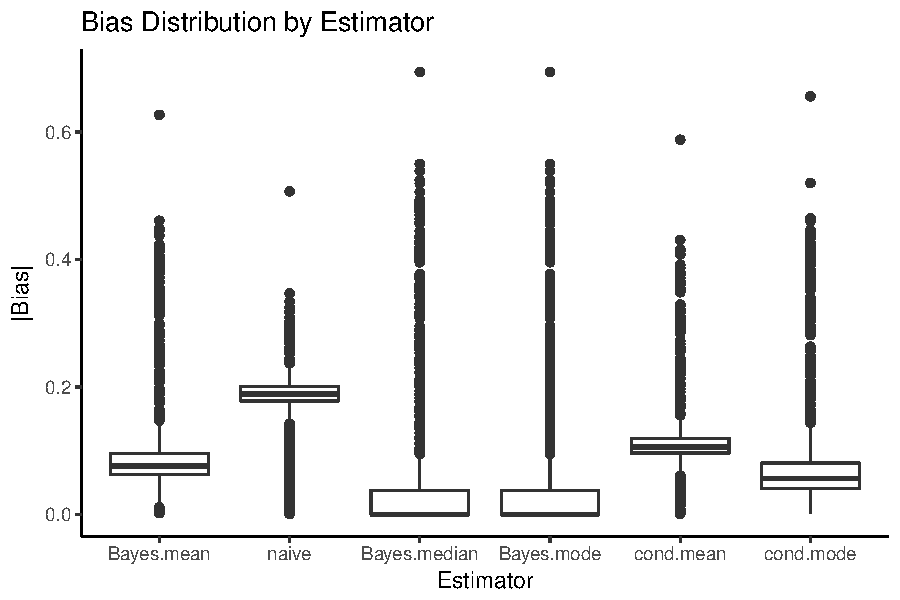
\includegraphics{thesis_files/figure-latex/unnamed-chunk-9-1.pdf}
\begin{verbatim}
          Lower       Upper                     
[1,] -0.2888934 -0.01643942 0.01344605 0.3483093
\end{verbatim}
\begin{Shaded}
\begin{Highlighting}[]
\KeywordTok{mean}\NormalTok{(p53.fulljags1.}\FloatTok{2.}\NormalTok{a}\OperatorTok{$}\NormalTok{BUGSoutput}\OperatorTok{$}\NormalTok{sims.list}\OperatorTok{$}\NormalTok{mu.p53)}
\end{Highlighting}
\end{Shaded}
\begin{verbatim}
[1] 0.04721087
\end{verbatim}
\begin{Shaded}
\begin{Highlighting}[]
\KeywordTok{median}\NormalTok{(p53.fulljags1.}\FloatTok{2.}\NormalTok{a}\OperatorTok{$}\NormalTok{BUGSoutput}\OperatorTok{$}\NormalTok{sims.list}\OperatorTok{$}\NormalTok{mu.p53)}
\end{Highlighting}
\end{Shaded}
\begin{verbatim}
[1] 0.06882402
\end{verbatim}
\begin{Shaded}
\begin{Highlighting}[]
\NormalTok{p53.fulljags1.}\FloatTok{2.}\NormalTok{i =}\StringTok{ }\KeywordTok{jags}\NormalTok{(}\DataTypeTok{data=}\NormalTok{sim.data1.}\DecValTok{2}\NormalTok{, ####this}
                    \DataTypeTok{inits=}\OtherTok{NULL}\NormalTok{, }\DataTypeTok{parameters.to.save =}\KeywordTok{c}\NormalTok{(}\StringTok{"pind"}\NormalTok{, }\StringTok{"mu.p53"}\NormalTok{, }\StringTok{"phi.p53"}\NormalTok{,}\StringTok{"mu.p53.notzero"}\NormalTok{),}
                    \DataTypeTok{model =}\NormalTok{ p53.test.ind)}
\end{Highlighting}
\end{Shaded}
\begin{verbatim}
Compiling model graph
   Resolving undeclared variables
   Allocating nodes
Graph information:
   Observed stochastic nodes: 700
   Unobserved stochastic nodes: 11
   Total graph size: 1468

Initializing model
\end{verbatim}
\begin{Shaded}
\begin{Highlighting}[]
\CommentTok{#par(mar=rep(1,4))}
\CommentTok{#plot(as.mcmc(p53.fulljags1.2.i))}
\KeywordTok{HPDM}\NormalTok{(p53.fulljags1.}\FloatTok{2.}\NormalTok{i}\OperatorTok{$}\NormalTok{BUGSoutput}\OperatorTok{$}\NormalTok{sims.list}\OperatorTok{$}\NormalTok{mu.p53, }\DataTypeTok{e=}\NormalTok{epsilon)}
\end{Highlighting}
\end{Shaded}
\begin{verbatim}


Potentially multimodal column vectors:
 1 

Column 1 multimodal intervals:  (-0.309,-0.01) (0.01,0.37) 
\end{verbatim}
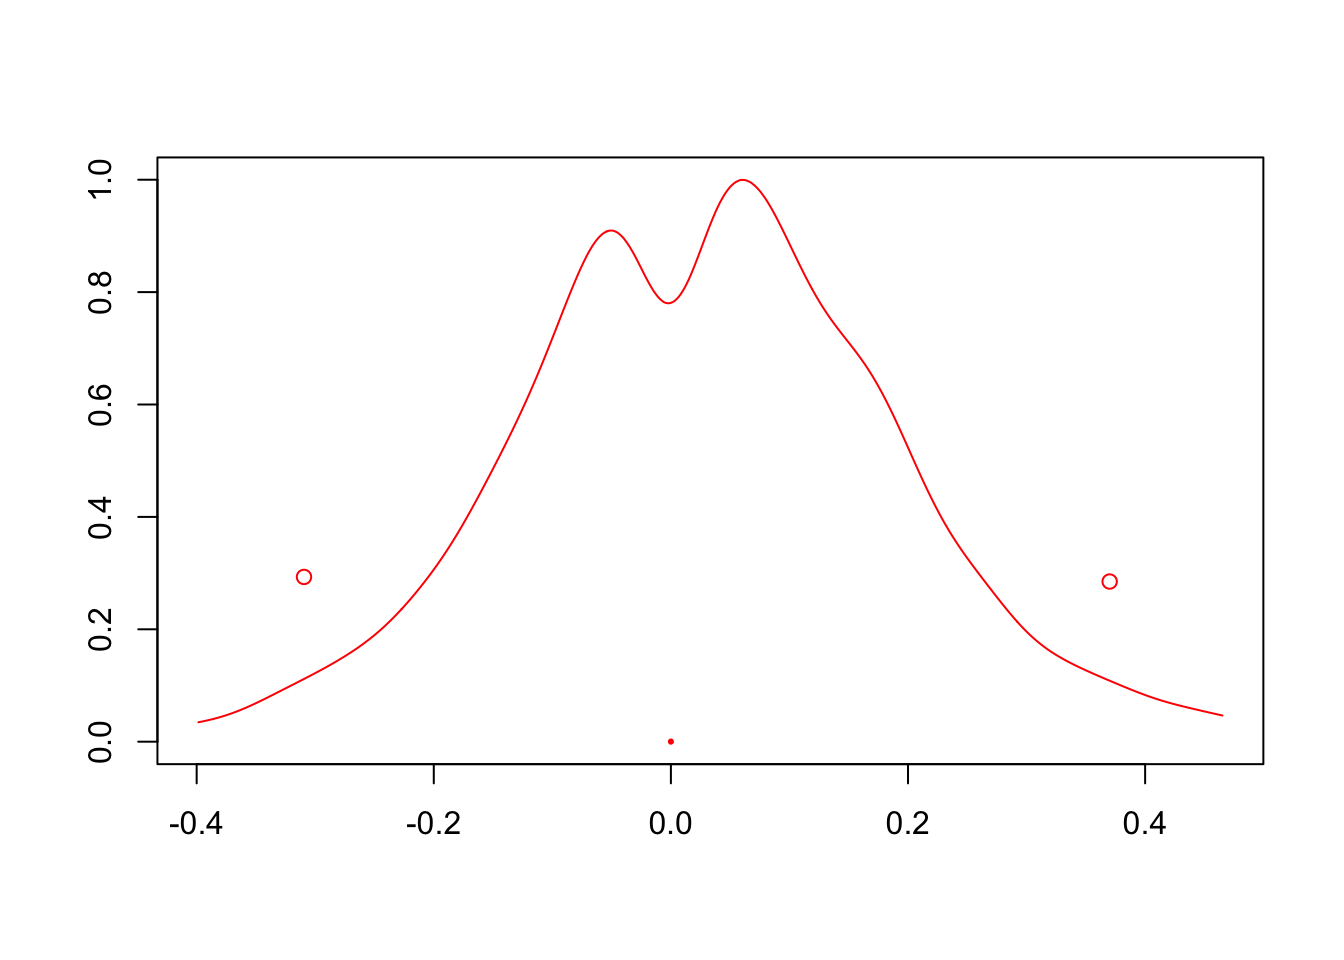
\includegraphics{thesis_files/figure-latex/unnamed-chunk-9-2.pdf}
\begin{verbatim}
          Lower       Upper                     
[1,] -0.3094696 -0.01022024 0.01006981 0.3700762
\end{verbatim}
\begin{Shaded}
\begin{Highlighting}[]
\KeywordTok{mean}\NormalTok{(p53.fulljags1.}\FloatTok{2.}\NormalTok{i}\OperatorTok{$}\NormalTok{BUGSoutput}\OperatorTok{$}\NormalTok{sims.list}\OperatorTok{$}\NormalTok{mu.p53)}
\end{Highlighting}
\end{Shaded}
\begin{verbatim}
[1] 0.03330651
\end{verbatim}
\begin{Shaded}
\begin{Highlighting}[]
\KeywordTok{median}\NormalTok{(p53.fulljags1.}\FloatTok{2.}\NormalTok{i}\OperatorTok{$}\NormalTok{BUGSoutput}\OperatorTok{$}\NormalTok{sims.list}\OperatorTok{$}\NormalTok{mu.p53)}
\end{Highlighting}
\end{Shaded}
\begin{verbatim}
[1] 0.03619337
\end{verbatim}
\begin{Shaded}
\begin{Highlighting}[]
\CommentTok{#glm}
\NormalTok{p53.fullglm1.}\DecValTok{2}\NormalTok{ =}\StringTok{ }\KeywordTok{glm}\NormalTok{(CaseCon }\OperatorTok{~}\StringTok{ }\KeywordTok{factor}\NormalTok{(site), }\DataTypeTok{data=}\NormalTok{sim.data1.}\DecValTok{2}\NormalTok{,  ####also this}
               \DataTypeTok{family=}\NormalTok{binomial, }\DataTypeTok{x=}\NormalTok{T)}

\KeywordTok{summary}\NormalTok{(p53.fullglm1.}\DecValTok{2}\NormalTok{)}
\end{Highlighting}
\end{Shaded}
\begin{verbatim}

Call:
glm(formula = CaseCon ~ factor(site), family = binomial, data = sim.data1.2, 
    x = T)

Deviance Residuals: 
   Min      1Q  Median      3Q     Max  
-1.335  -1.194   1.027   1.110   1.530  

Coefficients:
              Estimate Std. Error z value Pr(>|z|)  
(Intercept)    -0.1201     0.2004  -0.600   0.5487  
factor(site)2   0.2805     0.2836   0.989   0.3226  
factor(site)3  -0.6800     0.2948  -2.307   0.0211 *
factor(site)4   0.4841     0.2855   1.696   0.0899 .
factor(site)5   0.4841     0.2855   1.696   0.0899 .
factor(site)6   0.1601     0.2831   0.566   0.5716  
factor(site)7   0.2805     0.2836   0.989   0.3226  
---
Signif. codes:  0 '***' 0.001 '**' 0.01 '*' 0.05 '.' 0.1 ' ' 1

(Dispersion parameter for binomial family taken to be 1)

    Null deviance: 970.26  on 699  degrees of freedom
Residual deviance: 947.40  on 693  degrees of freedom
AIC: 961.4

Number of Fisher Scoring iterations: 4
\end{verbatim}
\begin{Shaded}
\begin{Highlighting}[]
\NormalTok{p53.fullglm1.}\FloatTok{2.}\NormalTok{simple =}\StringTok{ }\KeywordTok{glm}\NormalTok{(CaseCon }\OperatorTok{~}\StringTok{ }\DecValTok{1}\NormalTok{, }\DataTypeTok{data=}\NormalTok{sim.data1.}\DecValTok{2}\NormalTok{,  ####also this}
               \DataTypeTok{family=}\NormalTok{binomial, }\DataTypeTok{x=}\NormalTok{T)}

\KeywordTok{plot}\NormalTok{(}\KeywordTok{coef}\NormalTok{(p53.fullglm1.}\DecValTok{2}\NormalTok{), beta.p53.fixed.}\DecValTok{2}\NormalTok{)}
\KeywordTok{lines}\NormalTok{(}\KeywordTok{c}\NormalTok{(}\DecValTok{0}\NormalTok{,}\DecValTok{1}\NormalTok{),}\KeywordTok{c}\NormalTok{(}\DecValTok{0}\NormalTok{,}\DecValTok{1}\NormalTok{))}
\end{Highlighting}
\end{Shaded}
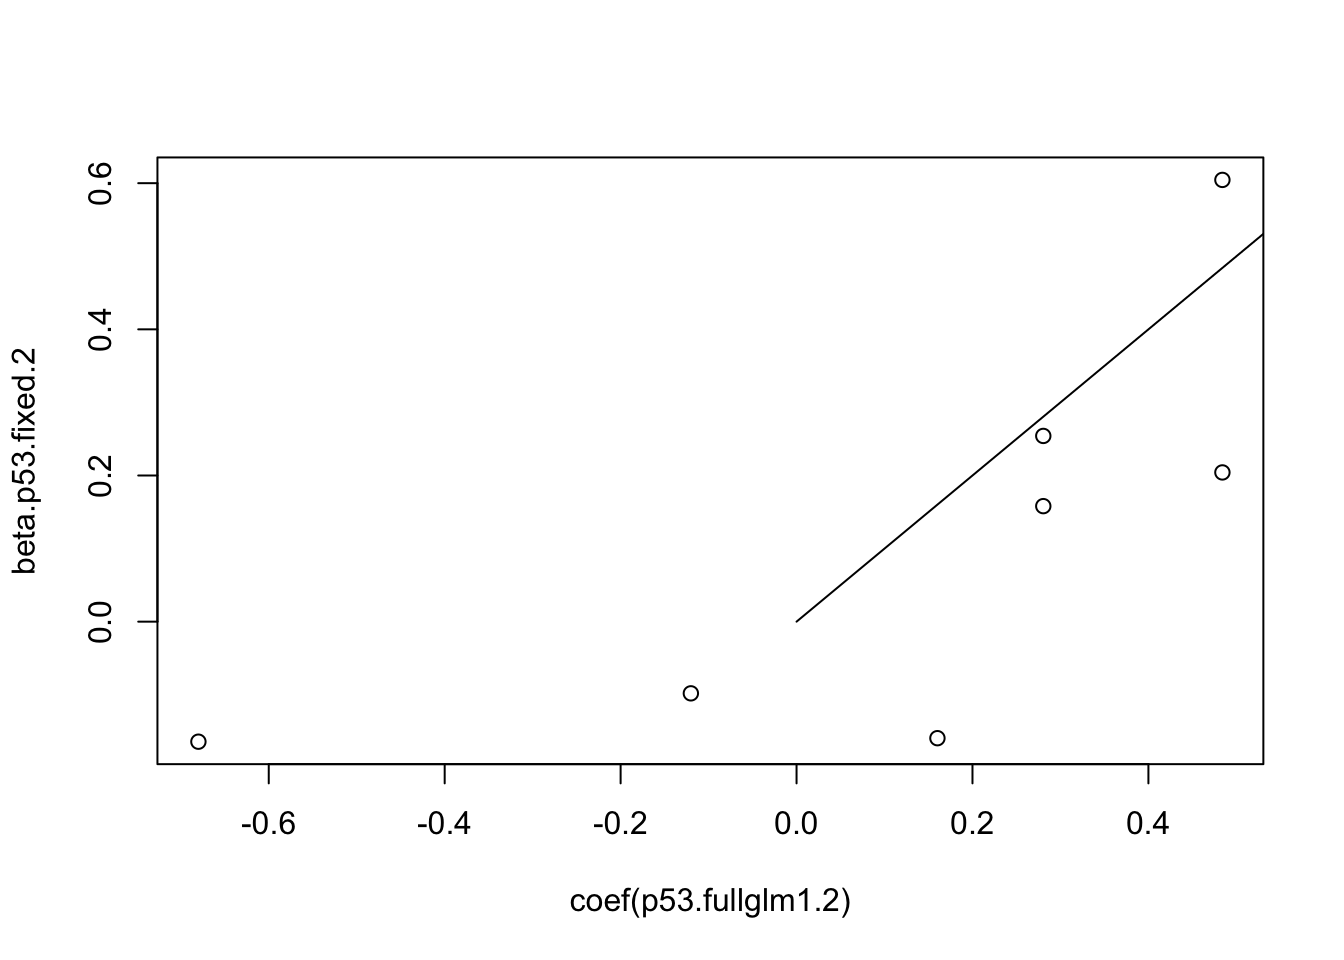
\includegraphics{thesis_files/figure-latex/unnamed-chunk-9-3.pdf} For
this \(\mu= 0.1\), the posterior appears to be in conflict with expected
behavior. However, upon observing the GLM coefficients we can see that
the true \(\beta_j\)'s were quite dispersed, and that the frequentist
and bayesian methods agree in expressing that there is a nonzero effect,
but it can positive or negative.
\begin{Shaded}
\begin{Highlighting}[]
\NormalTok{p53.fulljags1.}\FloatTok{0.}\NormalTok{l =}\StringTok{ }\KeywordTok{jags}\NormalTok{(}\DataTypeTok{data=}\NormalTok{sim.data1.}\DecValTok{0}\NormalTok{, ####this}
                    \DataTypeTok{inits=}\OtherTok{NULL}\NormalTok{, }\DataTypeTok{parameters.to.save =}\KeywordTok{c}\NormalTok{(}\StringTok{"pind"}\NormalTok{, }\StringTok{"mu.p53"}\NormalTok{, }\StringTok{"phi.p53"}\NormalTok{,}\StringTok{"mu.p53.notzero"}\NormalTok{,}\StringTok{"temp"}\NormalTok{,}\StringTok{"assoc"}\NormalTok{,}\StringTok{"mu1.p53"}\NormalTok{),}
                    \DataTypeTok{model =}\NormalTok{ p53.test.latent)}
\end{Highlighting}
\end{Shaded}
\begin{verbatim}
Compiling model graph
   Resolving undeclared variables
   Allocating nodes
Graph information:
   Observed stochastic nodes: 7000
   Unobserved stochastic nodes: 11
   Total graph size: 14056

Initializing model
\end{verbatim}
\begin{Shaded}
\begin{Highlighting}[]
\CommentTok{#par(mar=rep(1,4))}
\CommentTok{#plot(as.mcmc(p53.fulljags1.0.l))}
\KeywordTok{HPDM}\NormalTok{(p53.fulljags1.}\FloatTok{0.}\NormalTok{l}\OperatorTok{$}\NormalTok{BUGSoutput}\OperatorTok{$}\NormalTok{sims.list}\OperatorTok{$}\NormalTok{mu.p53, }\DataTypeTok{e=}\NormalTok{epsilon)}
\end{Highlighting}
\end{Shaded}
\begin{verbatim}
     Lower Upper
[1,]     0     0
\end{verbatim}
\begin{Shaded}
\begin{Highlighting}[]
\KeywordTok{mean}\NormalTok{(p53.fulljags1.}\FloatTok{0.}\NormalTok{l}\OperatorTok{$}\NormalTok{BUGSoutput}\OperatorTok{$}\NormalTok{sims.list}\OperatorTok{$}\NormalTok{mu.p53)}
\end{Highlighting}
\end{Shaded}
\begin{verbatim}
[1] 0
\end{verbatim}
\begin{Shaded}
\begin{Highlighting}[]
\KeywordTok{median}\NormalTok{(p53.fulljags1.}\FloatTok{0.}\NormalTok{l}\OperatorTok{$}\NormalTok{BUGSoutput}\OperatorTok{$}\NormalTok{sims.list}\OperatorTok{$}\NormalTok{mu.p53)}
\end{Highlighting}
\end{Shaded}
\begin{verbatim}
[1] 0
\end{verbatim}
\begin{Shaded}
\begin{Highlighting}[]
\CommentTok{#ones trick?}
\NormalTok{p53.test.latent.}\DecValTok{1}\NormalTok{=}\StringTok{ }\ControlFlowTok{function}\NormalTok{() \{}
  \ControlFlowTok{for}\NormalTok{ (j }\ControlFlowTok{in} \DecValTok{1}\OperatorTok{:}\NormalTok{J) \{}
\NormalTok{    CaseCon[j] }\OperatorTok{~}\StringTok{ }\KeywordTok{dbern}\NormalTok{(theta[j])}
    \KeywordTok{logit}\NormalTok{(theta[j]) <-}\StringTok{  }\NormalTok{beta.p53[site[j]]  \}}
  
  \ControlFlowTok{for}\NormalTok{ (l }\ControlFlowTok{in} \DecValTok{1}\OperatorTok{:}\NormalTok{n.sites) \{}
\NormalTok{    beta.p53.}\DecValTok{1}\NormalTok{[l] }\OperatorTok{~}\StringTok{ }\KeywordTok{dnorm}\NormalTok{(mu.p53, phi.p53)}
\NormalTok{    beta.p53[l] <-}\StringTok{ }\NormalTok{beta.p53.}\DecValTok{1}\NormalTok{[l]}\OperatorTok{*}\NormalTok{(mu.p53.notzero)}
\NormalTok{  \}}
  \CommentTok{#zeroes trick}
\NormalTok{  C<-}\FloatTok{1e6}
\NormalTok{  epsilon<-}\FloatTok{0.01}
\NormalTok{  tau<-}\StringTok{ }\KeywordTok{pow}\NormalTok{(epsilon,}\OperatorTok{-}\DecValTok{2}\NormalTok{)}
  \CommentTok{#if mu geq 0 and mu leq 0, prior is from point mass}
  \CommentTok{#is not zero if prob is greater}
\NormalTok{  mu.p53.notzero<-}\StringTok{ }\KeywordTok{step}\NormalTok{(temp)}
\NormalTok{  temp<-}\KeywordTok{dnorm}\NormalTok{(mu.p53,}\DecValTok{0}\NormalTok{,}\DecValTok{1}\NormalTok{)}\OperatorTok{-}\KeywordTok{dnorm}\NormalTok{(mu.p53,}\DecValTok{0}\NormalTok{,tau) }\CommentTok{#CHANGED precision to 1/4}
\NormalTok{  L<-(}\KeywordTok{dnorm}\NormalTok{(mu.p53,}\DecValTok{0}\NormalTok{,tau)}\OperatorTok{*}\NormalTok{(}\DecValTok{1}\OperatorTok{-}\NormalTok{pind))}\OperatorTok{+}\StringTok{ }\CommentTok{#(1- mu.p53.notzero)*(1-pind)+ #}
\StringTok{    }\NormalTok{(}\KeywordTok{dnorm}\NormalTok{(mu.p53,}\DecValTok{0}\NormalTok{,}\DecValTok{1}\NormalTok{)}\OperatorTok{*}\NormalTok{pind)}
\NormalTok{  p <-}\StringTok{ }\NormalTok{L}\OperatorTok{/}\StringTok{ }\NormalTok{C}
  \ControlFlowTok{for}\NormalTok{(i }\ControlFlowTok{in} \DecValTok{1}\OperatorTok{:}\NormalTok{n.ones)\{}
\NormalTok{    ones[i] }\OperatorTok{~}\StringTok{ }\KeywordTok{dbern}\NormalTok{(p)}

\NormalTok{  \}}
\NormalTok{  mu.p53 }\OperatorTok{~}\StringTok{ }\KeywordTok{dunif}\NormalTok{(}\OperatorTok{-}\DecValTok{10}\NormalTok{,}\DecValTok{10}\NormalTok{) }\CommentTok{#not sure how big this interval should be, just picked one large enough for .1 sd, started at 10, but even 1 has too large jumps}
  \CommentTok{#mu.p53<- mu1.p53*assoc}
  \CommentTok{#mu1.p53 ~ dnorm(0,1)}
\NormalTok{  phi.p53 }\OperatorTok{~}\StringTok{ }\KeywordTok{dgamma}\NormalTok{(}\DecValTok{1}\NormalTok{, .}\DecValTok{05}\NormalTok{)}
  \CommentTok{#    phi.p53 ~ dgamma(2, .02)}
\NormalTok{  sigma.p53 <-}\StringTok{ }\KeywordTok{pow}\NormalTok{(phi.p53, }\OperatorTok{-}\NormalTok{.}\DecValTok{5}\NormalTok{)}
  
  \CommentTok{#assoc~dbern(pind)}
\NormalTok{  pind }\OperatorTok{~}\StringTok{ }\KeywordTok{dbeta}\NormalTok{(.}\DecValTok{5}\NormalTok{,.}\DecValTok{5}\NormalTok{)}
\NormalTok{\}}

\NormalTok{n.ones=}\DecValTok{1}
\NormalTok{onesdata<-}\StringTok{ }\NormalTok{sim.data1.}\DecValTok{0}
\NormalTok{onesdata}\OperatorTok{$}\NormalTok{ones<-}\StringTok{ }\KeywordTok{rep}\NormalTok{(}\DecValTok{1}\NormalTok{,n.ones) }\CommentTok{#same}
\NormalTok{onesdata}\OperatorTok{$}\NormalTok{n.ones<-}\StringTok{ }\NormalTok{n.ones}
\NormalTok{p53.fulljags1.}\FloatTok{0.}\NormalTok{l1 =}\StringTok{ }\KeywordTok{jags}\NormalTok{(}\DataTypeTok{data=}\NormalTok{onesdata, ####this}
                    \DataTypeTok{inits=}\OtherTok{NULL}\NormalTok{, }\DataTypeTok{parameters.to.save =}\KeywordTok{c}\NormalTok{(}\StringTok{"pind"}\NormalTok{, }\StringTok{"mu.p53"}\NormalTok{, }\StringTok{"phi.p53"}\NormalTok{,}\StringTok{"mu.p53.notzero"}\NormalTok{,}\StringTok{"temp"}\NormalTok{),}
                    \DataTypeTok{model =}\NormalTok{ p53.test.latent.}\DecValTok{1}\NormalTok{)}
\end{Highlighting}
\end{Shaded}
\begin{verbatim}
Compiling model graph
   Resolving undeclared variables
   Allocating nodes
Graph information:
   Observed stochastic nodes: 7001
   Unobserved stochastic nodes: 10
   Total graph size: 14075

Initializing model
\end{verbatim}
\begin{Shaded}
\begin{Highlighting}[]
\CommentTok{#par(mar=rep(1,4))}
\CommentTok{#plot(as.mcmc(p53.fulljags1.0.l1))}
\KeywordTok{HPDM}\NormalTok{(p53.fulljags1.}\FloatTok{0.}\NormalTok{l}\OperatorTok{$}\NormalTok{BUGSoutput}\OperatorTok{$}\NormalTok{sims.list}\OperatorTok{$}\NormalTok{mu.p53, }\DataTypeTok{e=}\NormalTok{epsilon)}
\end{Highlighting}
\end{Shaded}
\begin{verbatim}
     Lower Upper
[1,]     0     0
\end{verbatim}
\begin{Shaded}
\begin{Highlighting}[]
\KeywordTok{mean}\NormalTok{(p53.fulljags1.}\FloatTok{0.}\NormalTok{l}\OperatorTok{$}\NormalTok{BUGSoutput}\OperatorTok{$}\NormalTok{sims.list}\OperatorTok{$}\NormalTok{mu.p53)}
\end{Highlighting}
\end{Shaded}
\begin{verbatim}
[1] 0
\end{verbatim}
\begin{Shaded}
\begin{Highlighting}[]
\KeywordTok{median}\NormalTok{(p53.fulljags1.}\FloatTok{0.}\NormalTok{l}\OperatorTok{$}\NormalTok{BUGSoutput}\OperatorTok{$}\NormalTok{sims.list}\OperatorTok{$}\NormalTok{mu.p53)}
\end{Highlighting}
\end{Shaded}
\begin{verbatim}
[1] 0
\end{verbatim}
Ones trick is still a little problematic, especially in trace of mu
\begin{Shaded}
\begin{Highlighting}[]
\NormalTok{p53.fulljags1.}\FloatTok{1.}\NormalTok{l =}\StringTok{ }\KeywordTok{jags}\NormalTok{(}\DataTypeTok{data=}\NormalTok{sim.data1.}\DecValTok{1}\NormalTok{, ####this}
                    \DataTypeTok{inits=}\OtherTok{NULL}\NormalTok{, }\DataTypeTok{parameters.to.save =}\KeywordTok{c}\NormalTok{(}\StringTok{"pind"}\NormalTok{, }\StringTok{"mu.p53"}\NormalTok{, }\StringTok{"phi.p53"}\NormalTok{,}\StringTok{"mu.p53.notzero"}\NormalTok{,}\StringTok{"temp"}\NormalTok{,}\StringTok{"assoc"}\NormalTok{,}\StringTok{"mu1.p53"}\NormalTok{),}
                    \DataTypeTok{model =}\NormalTok{ p53.test.latent)}
\end{Highlighting}
\end{Shaded}
\begin{verbatim}
Compiling model graph
   Resolving undeclared variables
   Allocating nodes
Graph information:
   Observed stochastic nodes: 7000
   Unobserved stochastic nodes: 11
   Total graph size: 14056

Initializing model
\end{verbatim}
\begin{Shaded}
\begin{Highlighting}[]
\CommentTok{#par(mar=rep(1,4))}
\CommentTok{#plot(as.mcmc(p53.fulljags1.1.l))}
\KeywordTok{HPDM}\NormalTok{(p53.fulljags1.}\FloatTok{1.}\NormalTok{l}\OperatorTok{$}\NormalTok{BUGSoutput}\OperatorTok{$}\NormalTok{sims.list}\OperatorTok{$}\NormalTok{mu.p53, }\DataTypeTok{e=}\NormalTok{epsilon)}
\end{Highlighting}
\end{Shaded}
\begin{verbatim}
         Lower     Upper
[1,] 0.2759939 0.6766949
\end{verbatim}
\begin{Shaded}
\begin{Highlighting}[]
\KeywordTok{mean}\NormalTok{(p53.fulljags1.}\FloatTok{1.}\NormalTok{l}\OperatorTok{$}\NormalTok{BUGSoutput}\OperatorTok{$}\NormalTok{sims.list}\OperatorTok{$}\NormalTok{mu.p53)}
\end{Highlighting}
\end{Shaded}
\begin{verbatim}
[1] 0.4783651
\end{verbatim}
\begin{Shaded}
\begin{Highlighting}[]
\KeywordTok{median}\NormalTok{(p53.fulljags1.}\FloatTok{1.}\NormalTok{l}\OperatorTok{$}\NormalTok{BUGSoutput}\OperatorTok{$}\NormalTok{sims.list}\OperatorTok{$}\NormalTok{mu.p53)}
\end{Highlighting}
\end{Shaded}
\begin{verbatim}
[1] 0.4795407
\end{verbatim}
\begin{Shaded}
\begin{Highlighting}[]
\NormalTok{p53.fulljags1.}\FloatTok{2.}\NormalTok{l =}\StringTok{ }\KeywordTok{jags}\NormalTok{(}\DataTypeTok{data=}\NormalTok{sim.data1.}\DecValTok{2}\NormalTok{, ####this}
                    \DataTypeTok{inits=}\OtherTok{NULL}\NormalTok{, }\DataTypeTok{parameters.to.save =}\KeywordTok{c}\NormalTok{(}\StringTok{"pind"}\NormalTok{, }\StringTok{"mu.p53"}\NormalTok{, }\StringTok{"phi.p53"}\NormalTok{,}\StringTok{"mu.p53.notzero"}\NormalTok{,}\StringTok{"temp"}\NormalTok{,}\StringTok{"assoc"}\NormalTok{,}\StringTok{"mu1.p53"}\NormalTok{),}
                    \DataTypeTok{model =}\NormalTok{ p53.test.latent)}
\end{Highlighting}
\end{Shaded}
\begin{verbatim}
Compiling model graph
   Resolving undeclared variables
   Allocating nodes
Graph information:
   Observed stochastic nodes: 700
   Unobserved stochastic nodes: 11
   Total graph size: 1456

Initializing model
\end{verbatim}
\begin{Shaded}
\begin{Highlighting}[]
\CommentTok{#par(mar=rep(1,4))}
\CommentTok{#plot(as.mcmc(p53.fulljags1.2.l))}
\KeywordTok{HPDM}\NormalTok{(p53.fulljags1.}\FloatTok{2.}\NormalTok{l}\OperatorTok{$}\NormalTok{BUGSoutput}\OperatorTok{$}\NormalTok{sims.list}\OperatorTok{$}\NormalTok{mu.p53, }\DataTypeTok{e=}\NormalTok{epsilon)}
\end{Highlighting}
\end{Shaded}
\begin{verbatim}


Potentially multimodal column vectors:
 1 

Column 1 multimodal intervals:  (-0.262,0.305) 
\end{verbatim}
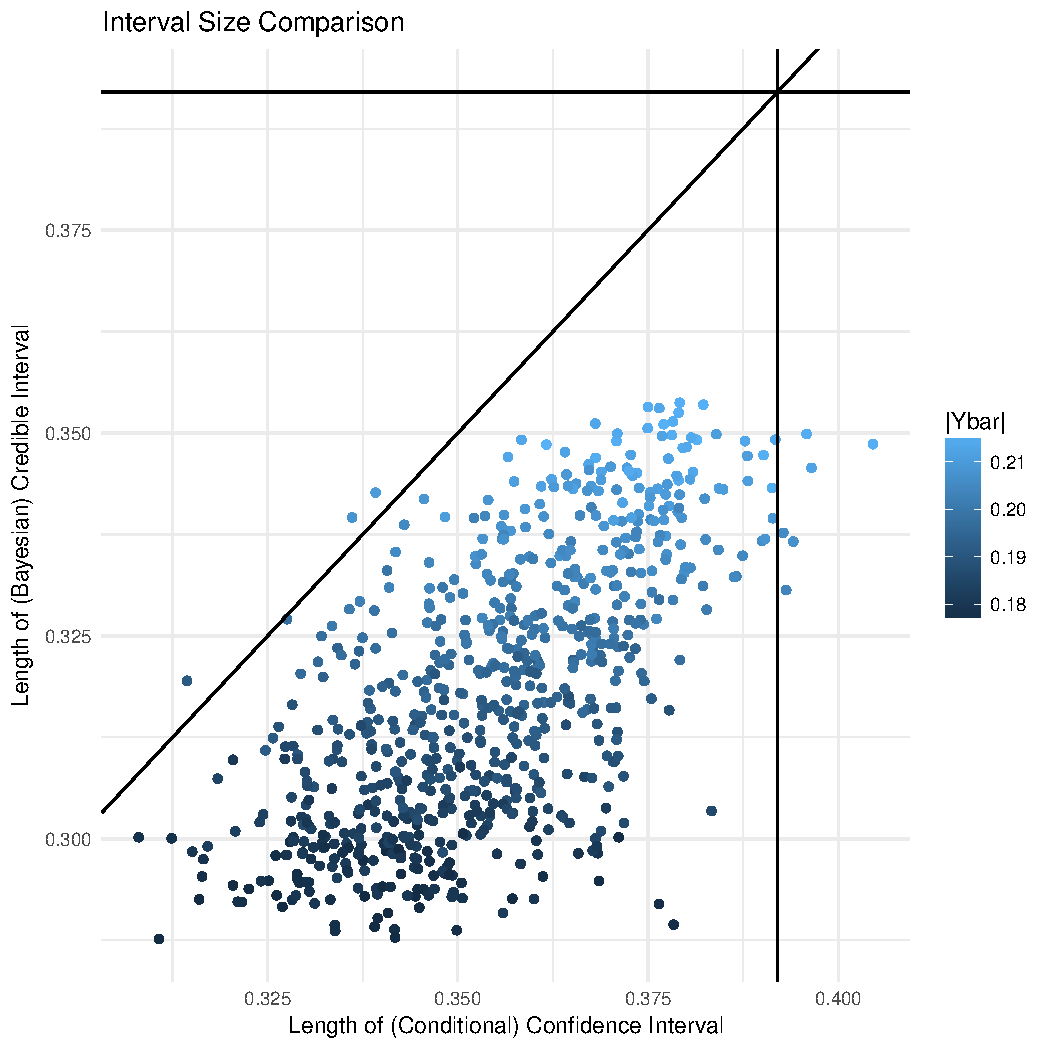
\includegraphics{thesis_files/figure-latex/unnamed-chunk-13-1.pdf}
\begin{verbatim}
         Lower     Upper
[1,] -0.262373 0.3048219
\end{verbatim}
\begin{Shaded}
\begin{Highlighting}[]
\KeywordTok{mean}\NormalTok{(p53.fulljags1.}\FloatTok{2.}\NormalTok{l}\OperatorTok{$}\NormalTok{BUGSoutput}\OperatorTok{$}\NormalTok{sims.list}\OperatorTok{$}\NormalTok{mu.p53)}
\end{Highlighting}
\end{Shaded}
\begin{verbatim}
[1] 0.02193662
\end{verbatim}
\begin{Shaded}
\begin{Highlighting}[]
\KeywordTok{median}\NormalTok{(p53.fulljags1.}\FloatTok{2.}\NormalTok{l}\OperatorTok{$}\NormalTok{BUGSoutput}\OperatorTok{$}\NormalTok{sims.list}\OperatorTok{$}\NormalTok{mu.p53)}
\end{Highlighting}
\end{Shaded}
\begin{verbatim}
[1] 0
\end{verbatim}
\begin{Shaded}
\begin{Highlighting}[]
\CommentTok{#precision=4}
\NormalTok{onesdata<-}\StringTok{ }\NormalTok{sim.data1.}\DecValTok{2}
\NormalTok{onesdata}\OperatorTok{$}\NormalTok{n.ones<-}\DecValTok{1}
\NormalTok{onesdata}\OperatorTok{$}\NormalTok{ones<-}\StringTok{ }\KeywordTok{rep}\NormalTok{(}\DecValTok{1}\NormalTok{, onesdata}\OperatorTok{$}\NormalTok{n.ones)}
\NormalTok{p53.fulljags1.}\FloatTok{2.}\NormalTok{l1 =}\StringTok{ }\KeywordTok{jags}\NormalTok{(}\DataTypeTok{data=}\NormalTok{onesdata, ####this}
                    \DataTypeTok{inits=}\OtherTok{NULL}\NormalTok{, }\DataTypeTok{parameters.to.save =}\KeywordTok{c}\NormalTok{(}\StringTok{"pind"}\NormalTok{, }\StringTok{"mu.p53"}\NormalTok{, }\StringTok{"phi.p53"}\NormalTok{,}\StringTok{"mu.p53.notzero"}\NormalTok{,}\StringTok{"temp"}\NormalTok{),}
                    \DataTypeTok{model =}\NormalTok{ p53.test.latent.}\DecValTok{1}\NormalTok{)}
\end{Highlighting}
\end{Shaded}
\begin{verbatim}
Compiling model graph
   Resolving undeclared variables
   Allocating nodes
Graph information:
   Observed stochastic nodes: 701
   Unobserved stochastic nodes: 10
   Total graph size: 1475

Initializing model
\end{verbatim}
\begin{Shaded}
\begin{Highlighting}[]
\CommentTok{#par(mar=rep(1,4))}
\CommentTok{#plot(as.mcmc(p53.fulljags1.2.l1))}
\end{Highlighting}
\end{Shaded}
\begin{Shaded}
\begin{Highlighting}[]
\CommentTok{#with precision = .25}
\NormalTok{p53.fulljags1.}\FloatTok{2.}\NormalTok{l2 =}\StringTok{ }\KeywordTok{jags}\NormalTok{(}\DataTypeTok{data=}\NormalTok{onesdata, ####this}
                    \DataTypeTok{inits=}\OtherTok{NULL}\NormalTok{, }\DataTypeTok{parameters.to.save =}\KeywordTok{c}\NormalTok{(}\StringTok{"pind"}\NormalTok{, }\StringTok{"mu.p53"}\NormalTok{, }\StringTok{"phi.p53"}\NormalTok{,}\StringTok{"mu.p53.notzero"}\NormalTok{,}\StringTok{"temp"}\NormalTok{),}
                    \DataTypeTok{model =}\NormalTok{ p53.test.latent.}\DecValTok{1}\NormalTok{)}
\end{Highlighting}
\end{Shaded}
\begin{verbatim}
Compiling model graph
   Resolving undeclared variables
   Allocating nodes
Graph information:
   Observed stochastic nodes: 701
   Unobserved stochastic nodes: 10
   Total graph size: 1475

Initializing model
\end{verbatim}
\begin{Shaded}
\begin{Highlighting}[]
\CommentTok{#par(mar=rep(1,4))}
\CommentTok{#plot(as.mcmc(p53.fulljags1.2.l2))}
\end{Highlighting}
\end{Shaded}
This last simulation is an example of Bartlett's paradox: the nonzero
part of the prior is too diffuse, and so the zero component ends up
being favored.

\chapter{Application}\label{application}
\begin{Shaded}
\begin{Highlighting}[]
\NormalTok{knitr}\OperatorTok{::}\NormalTok{opts_chunk}\OperatorTok{$}\KeywordTok{set}\NormalTok{(}\DataTypeTok{echo =} \OtherTok{TRUE}\NormalTok{)}
\NormalTok{knitr}\OperatorTok{::}\NormalTok{opts_chunk}\OperatorTok{$}\KeywordTok{set}\NormalTok{(}\DataTypeTok{cache =} \OtherTok{TRUE}\NormalTok{)}

\KeywordTok{library}\NormalTok{(rmeta)}
\KeywordTok{library}\NormalTok{(lme4)}
\KeywordTok{library}\NormalTok{(}\StringTok{"R2jags"}\NormalTok{)}
\KeywordTok{library}\NormalTok{(xtable)}
\end{Highlighting}
\end{Shaded}
\section{Genome Study}\label{genome-study}
\begin{itemize}
\tightlist
\item
  description from previous papers
\end{itemize}
\begin{Shaded}
\begin{Highlighting}[]
\KeywordTok{load}\NormalTok{(}\StringTok{"tp53.Rdata"}\NormalTok{)}
\NormalTok{getdata<-}\StringTok{ }\ControlFlowTok{function}\NormalTok{(snp.name, }\DataTypeTok{iter=}\DecValTok{5000}\NormalTok{, }\DataTypeTok{drop=} \OtherTok{NULL}\NormalTok{)\{}
  
 \CommentTok{#more iterations, coda traceplots, maybe look at the prior still- cauchy prior? ideally would do joint update (check if model is reducible-> chain gets stuck)-> maube google this bc jags probably }
 \CommentTok{#}


\ControlFlowTok{if}\NormalTok{(}\OperatorTok{!}\KeywordTok{is.null}\NormalTok{(drop)) \{}
\NormalTok{  use =}\StringTok{ }\OperatorTok{!}\NormalTok{(tp53epi.wsi}\OperatorTok{$}\NormalTok{site }\OperatorTok\StringTok{ }\NormalTok{drop)}
\NormalTok{  \} }\ControlFlowTok{else}\NormalTok{ \{}
\NormalTok{    use =}\StringTok{ }\KeywordTok{rep}\NormalTok{(}\OtherTok{TRUE}\NormalTok{, }\KeywordTok{nrow}\NormalTok{(tp53epi.wsi))}
\NormalTok{  \}}
  
\NormalTok{  p53.snp =}\StringTok{ }\NormalTok{tp53geno.wsi[use, snp.name]}
\NormalTok{  tp53epi.wsi =}\StringTok{ }\NormalTok{tp53epi.wsi[use,]}
  
\NormalTok{  missing.geno =}\StringTok{ }\KeywordTok{is.na}\NormalTok{(p53.snp)}
\NormalTok{  site.names =}\StringTok{ }\KeywordTok{levels}\NormalTok{(}\KeywordTok{factor}\NormalTok{(tp53epi.wsi[}\OperatorTok{!}\NormalTok{missing.geno,}\StringTok{"site"}\NormalTok{]))}

\NormalTok{  p53.data =}\StringTok{ }\KeywordTok{list}\NormalTok{(}\DataTypeTok{CaseCon=}\NormalTok{tp53epi.wsi}\OperatorTok{$}\NormalTok{casecon[}\OperatorTok{!}\NormalTok{missing.geno], }\DataTypeTok{site=}\KeywordTok{as.numeric}\NormalTok{(}\KeywordTok{factor}\NormalTok{(tp53epi.wsi}\OperatorTok{$}\NormalTok{site[}\OperatorTok{!}\NormalTok{missing.geno])), }\DataTypeTok{BC =} \KeywordTok{as.numeric}\NormalTok{(tp53epi.wsi}\OperatorTok{$}\NormalTok{prev.BC[}\OperatorTok{!}\NormalTok{missing.geno]), }\DataTypeTok{Age =}\NormalTok{ tp53epi.wsi}\OperatorTok{$}\NormalTok{refage[}\OperatorTok{!}\NormalTok{missing.geno], }\DataTypeTok{p53 =}\NormalTok{ p53.snp[}\OperatorTok{!}\NormalTok{missing.geno])}

\NormalTok{  p53.df =}\StringTok{ }\KeywordTok{data.frame}\NormalTok{(p53.data)}

\NormalTok{  J =}\StringTok{ }\KeywordTok{length}\NormalTok{(p53.data}\OperatorTok{$}\NormalTok{CaseCon)}
\NormalTok{  n.sites =}\StringTok{ }\KeywordTok{length}\NormalTok{(}\KeywordTok{unique}\NormalTok{(p53.data}\OperatorTok{$}\NormalTok{site))}
\NormalTok{  p53.data}\OperatorTok{$}\NormalTok{J =}\StringTok{ }\NormalTok{J}
\NormalTok{  p53.data}\OperatorTok{$}\NormalTok{n.sites =}\StringTok{ }\NormalTok{n.sites}
  
  \CommentTok{#this is a new indicator}
\NormalTok{  p53.data}\OperatorTok{$}\NormalTok{discovery.sites <-}\StringTok{ }\KeywordTok{which}\NormalTok{(}\KeywordTok{levels}\NormalTok{(}\KeywordTok{factor}\NormalTok{(tp53epi.wsi}\OperatorTok{$}\NormalTok{site))}\OperatorTok\StringTok{ }\NormalTok{drop)}
\NormalTok{  p53.data}\OperatorTok{$}\NormalTok{missing.geno<-missing.geno}
  
  \KeywordTok{return}\NormalTok{(p53.data)}
  
\NormalTok{\}}

\NormalTok{snp.name=}\StringTok{"rs12951053n"}
\NormalTok{discovery.sitenames=}\StringTok{ }\KeywordTok{c}\NormalTok{(}\StringTok{"POL"}\NormalTok{, }\StringTok{"MAY"}\NormalTok{, }\StringTok{"NCO"}\NormalTok{)}
\CommentTok{#regular data}
\NormalTok{p53.data<-}\StringTok{ }\KeywordTok{getdata}\NormalTok{(snp.name)}
\CommentTok{#validation data}
\NormalTok{p53.dataval<-}\StringTok{ }\KeywordTok{getdata}\NormalTok{(snp.name, }\DataTypeTok{drop=}\NormalTok{discovery.sitenames)}
\end{Highlighting}
\end{Shaded}
\begin{Shaded}
\begin{Highlighting}[]
\KeywordTok{source}\NormalTok{(}\StringTok{"HPD.R"}\NormalTok{)}
\end{Highlighting}
\end{Shaded}
\subsection{EDA}\label{eda}
\begin{itemize}
\item
  plot of data points?
\item
  conditional likelihood, FDR, etc as function of Y
\item
\end{itemize}
\begin{Shaded}
\begin{Highlighting}[]
\NormalTok{OR.freq =}\StringTok{ }\ControlFlowTok{function}\NormalTok{(snp.name, tp53epi.wsi,tp53geno.wsi, }\DataTypeTok{psdir=}\StringTok{"ps"}\NormalTok{, }\DataTypeTok{drop=}\OtherTok{NULL}\NormalTok{,}\DataTypeTok{iter=}\DecValTok{5000}\NormalTok{, }\DataTypeTok{debug=}\NormalTok{F) \{}

  \ControlFlowTok{if}\NormalTok{ (}\OperatorTok{!}\KeywordTok{is.null}\NormalTok{(drop)) \{}
\NormalTok{    use =}\StringTok{ }\OperatorTok{!}\NormalTok{(tp53epi.wsi}\OperatorTok{$}\NormalTok{site }\OperatorTok\StringTok{ }\NormalTok{drop)\}}
  \ControlFlowTok{else}\NormalTok{ \{}
\NormalTok{    use =}\StringTok{ }\KeywordTok{rep}\NormalTok{(}\OtherTok{TRUE}\NormalTok{, }\KeywordTok{nrow}\NormalTok{(tp53epi.wsi))}
\NormalTok{  \}}
  
\NormalTok{  p53.snp =}\StringTok{ }\NormalTok{tp53geno.wsi[use, snp.name]}
\NormalTok{  tp53epi.wsi =}\StringTok{ }\NormalTok{tp53epi.wsi[use,]}
  
\NormalTok{  missing.geno =}\StringTok{ }\KeywordTok{is.na}\NormalTok{(p53.snp)}
\NormalTok{  site.names =}\StringTok{ }\KeywordTok{levels}\NormalTok{(}\KeywordTok{factor}\NormalTok{(tp53epi.wsi[}\OperatorTok{!}\NormalTok{missing.geno,}\StringTok{"site"}\NormalTok{]))}

\NormalTok{  p53.data =}\StringTok{ }\KeywordTok{list}\NormalTok{(}\DataTypeTok{CaseCon=}\NormalTok{tp53epi.wsi}\OperatorTok{$}\NormalTok{casecon[}\OperatorTok{!}\NormalTok{missing.geno], }\DataTypeTok{site=}\KeywordTok{as.numeric}\NormalTok{(}\KeywordTok{factor}\NormalTok{(tp53epi.wsi}\OperatorTok{$}\NormalTok{site[}\OperatorTok{!}\NormalTok{missing.geno])), }\DataTypeTok{BC =} \KeywordTok{as.numeric}\NormalTok{(tp53epi.wsi}\OperatorTok{$}\NormalTok{prev.BC[}\OperatorTok{!}\NormalTok{missing.geno]), }\DataTypeTok{Age =}\NormalTok{ tp53epi.wsi}\OperatorTok{$}\NormalTok{refage[}\OperatorTok{!}\NormalTok{missing.geno], }\DataTypeTok{p53 =}\NormalTok{ p53.snp[}\OperatorTok{!}\NormalTok{missing.geno])}

\NormalTok{  p53.df =}\StringTok{ }\KeywordTok{data.frame}\NormalTok{(p53.data)}
  \KeywordTok{write.csv}\NormalTok{(p53.df, }\DataTypeTok{file=}\KeywordTok{paste}\NormalTok{(snp.name, }\StringTok{".csv"}\NormalTok{, }\DataTypeTok{sep=}\StringTok{""}\NormalTok{))}
  
\NormalTok{  p53.full =}\StringTok{ }\KeywordTok{glm}\NormalTok{(CaseCon }\OperatorTok{~}\StringTok{ }\KeywordTok{factor}\NormalTok{(site) }\OperatorTok{+}\StringTok{ }\KeywordTok{factor}\NormalTok{(site)}\OperatorTok{*}\NormalTok{p53 }\OperatorTok{+}\StringTok{ }\KeywordTok{factor}\NormalTok{(site)}\OperatorTok{*}\NormalTok{Age }\OperatorTok{+}\StringTok{ }\NormalTok{BC, }\DataTypeTok{data=}\NormalTok{p53.df, }\DataTypeTok{family=}\NormalTok{binomial, }\DataTypeTok{x=}\NormalTok{T)}
\NormalTok{ p53.pooled =}\StringTok{ }\KeywordTok{glm}\NormalTok{(CaseCon }\OperatorTok{~}\StringTok{ }\KeywordTok{factor}\NormalTok{(site) }\OperatorTok{+}\StringTok{ }\NormalTok{p53 }\OperatorTok{+}\StringTok{ }\KeywordTok{factor}\NormalTok{(site)}\OperatorTok{*}\NormalTok{Age }\OperatorTok{+}\StringTok{ }\NormalTok{BC, }\DataTypeTok{data=}\NormalTok{p53.df, }\DataTypeTok{family=}\NormalTok{binomial)}
\NormalTok{   p53.null =}\StringTok{ }\KeywordTok{glm}\NormalTok{(CaseCon }\OperatorTok{~}\StringTok{ }\KeywordTok{factor}\NormalTok{(site) }\OperatorTok{+}\StringTok{  }\KeywordTok{factor}\NormalTok{(site)}\OperatorTok{*}\NormalTok{Age }\OperatorTok{+}\StringTok{ }\NormalTok{BC, }\DataTypeTok{data=}\NormalTok{p53.df, }\DataTypeTok{family=}\NormalTok{binomial)}

\NormalTok{  p53.df}\OperatorTok{$}\NormalTok{Site =}\StringTok{ }\KeywordTok{factor}\NormalTok{(p53.df}\OperatorTok{$}\NormalTok{site)}

\NormalTok{  p53.me =}\StringTok{ }\KeywordTok{glmer}\NormalTok{(CaseCon }\OperatorTok{~}\StringTok{ }\NormalTok{BC }\OperatorTok{+}\StringTok{ }\NormalTok{p53 }\OperatorTok{+}\StringTok{ }\NormalTok{Age }\OperatorTok{+}\StringTok{ }\NormalTok{(}\DecValTok{1}\OperatorTok{|}\NormalTok{site)  }\OperatorTok{+}\StringTok{ }\NormalTok{(}\DecValTok{0} \OperatorTok{+}\StringTok{ }\NormalTok{p53 }\OperatorTok{|}\StringTok{ }\NormalTok{site) }\OperatorTok{+}\StringTok{ }\NormalTok{(}\DecValTok{0} \OperatorTok{+}\StringTok{ }\NormalTok{Age }\OperatorTok{|}\StringTok{ }\NormalTok{site), }\DataTypeTok{start=}\KeywordTok{c}\NormalTok{(}\DataTypeTok{site=}\FloatTok{1.0}\NormalTok{, }\DataTypeTok{p53=}\NormalTok{.}\DecValTok{1}\NormalTok{, }\DataTypeTok{Age=}\NormalTok{.}\DecValTok{01}\NormalTok{),}\DataTypeTok{nAGQ=}\DecValTok{1}\NormalTok{ , }\DataTypeTok{data=}\NormalTok{p53.df, }\DataTypeTok{family=}\NormalTok{binomial)}

\NormalTok{  test=}\KeywordTok{anova}\NormalTok{(p53.full, p53.pooled, p53.null, }\DataTypeTok{test=}\StringTok{"Chi"}\NormalTok{)}
\NormalTok{  coef =}\StringTok{ }\KeywordTok{summary}\NormalTok{(p53.full)}\OperatorTok{$}\NormalTok{coef}
\NormalTok{  ns =}\StringTok{ }\KeywordTok{length}\NormalTok{(site.names)}
\NormalTok{  OR =}\StringTok{ }\NormalTok{coef[}\KeywordTok{c}\NormalTok{(ns}\OperatorTok{+}\DecValTok{1}\NormalTok{, (ns}\OperatorTok{+}\DecValTok{4}\NormalTok{)}\OperatorTok{:}\NormalTok{(ns}\OperatorTok{+}\NormalTok{ns}\OperatorTok{+}\DecValTok{2}\NormalTok{)),}\DecValTok{1}\NormalTok{]}
\NormalTok{  x =}\StringTok{ }\NormalTok{p53.full}\OperatorTok{$}\NormalTok{x}
\NormalTok{  p =}\StringTok{ }\KeywordTok{predict}\NormalTok{(p53.full, }\DataTypeTok{type=}\StringTok{"response"}\NormalTok{)}
\NormalTok{  var =}\StringTok{ }\KeywordTok{solve}\NormalTok{(}\KeywordTok{t}\NormalTok{(x)}\OperatorTok\StringTok{ }\KeywordTok{diag}\NormalTok{(p}\OperatorTok{*}\NormalTok{(}\DecValTok{1}\OperatorTok{-}\NormalTok{p)) }\OperatorTok\NormalTok{x)[}\KeywordTok{c}\NormalTok{(ns}\OperatorTok{+}\DecValTok{1}\NormalTok{, (ns}\OperatorTok{+}\DecValTok{4}\NormalTok{)}\OperatorTok{:}\NormalTok{(ns}\OperatorTok{+}\NormalTok{ns}\OperatorTok{+}\DecValTok{2}\NormalTok{)),}\KeywordTok{c}\NormalTok{(ns}\OperatorTok{+}\DecValTok{1}\NormalTok{, (ns}\OperatorTok{+}\DecValTok{4}\NormalTok{)}\OperatorTok{:}\NormalTok{(ns}\OperatorTok{+}\NormalTok{ns}\OperatorTok{+}\DecValTok{2}\NormalTok{))]}

  \KeywordTok{sqrt}\NormalTok{(}\KeywordTok{diag}\NormalTok{(var))}

\NormalTok{  eff =}\StringTok{ }\KeywordTok{matrix}\NormalTok{(}\DecValTok{0}\NormalTok{, ns,ns)}
\NormalTok{  eff[,}\DecValTok{1}\NormalTok{] =}\StringTok{ }\DecValTok{1}
  \ControlFlowTok{for}\NormalTok{ (i }\ControlFlowTok{in} \DecValTok{2}\OperatorTok{:}\NormalTok{ns) eff[i,i] =}\StringTok{ }\DecValTok{1}

\NormalTok{  OR =}\StringTok{ }\NormalTok{eff }\OperatorTok\StringTok{ }\NormalTok{OR}
\NormalTok{  OR.SE =}\StringTok{ }\KeywordTok{sqrt}\NormalTok{(}\KeywordTok{diag}\NormalTok{(eff }\OperatorTok\StringTok{ }\NormalTok{var }\OperatorTok\StringTok{ }\KeywordTok{t}\NormalTok{(eff)))}
  
\NormalTok{  DS =}\StringTok{ }\KeywordTok{meta.summaries}\NormalTok{(OR, OR.SE, }\DataTypeTok{method=}\StringTok{"random"}\NormalTok{, }\DataTypeTok{names=}\NormalTok{site.names, }\DataTypeTok{logscale=}\NormalTok{F)}
\NormalTok{  p.value =}\StringTok{ }\KeywordTok{pnorm}\NormalTok{(}\OperatorTok{-}\NormalTok{(}\KeywordTok{abs}\NormalTok{(DS}\OperatorTok{$}\NormalTok{summary}\OperatorTok{/}\NormalTok{DS}\OperatorTok{$}\NormalTok{se.summary)))}\OperatorTok{*}\DecValTok{2}
\NormalTok{  BF0 =}\StringTok{ }\OperatorTok{-}\KeywordTok{exp}\NormalTok{(}\DecValTok{1}\NormalTok{)}\OperatorTok{*}\NormalTok{p.value}\OperatorTok{*}\KeywordTok{log}\NormalTok{(p.value)}
  \KeywordTok{return}\NormalTok{(}\KeywordTok{list}\NormalTok{(}\DataTypeTok{snp=}\NormalTok{snp.name, }\DataTypeTok{DS=}\NormalTok{DS, }\DataTypeTok{OR=}\NormalTok{OR, }\DataTypeTok{SE=}\NormalTok{OR.SE, }\DataTypeTok{p.value=}\NormalTok{p.value, }\DataTypeTok{BF.Ha =} \DecValTok{1}\OperatorTok{/}\NormalTok{BF0, }\DataTypeTok{test=}\NormalTok{test, }\DataTypeTok{p53.me=}\NormalTok{p53.me))}
\NormalTok{\}}
\end{Highlighting}
\end{Shaded}
\begin{Shaded}
\begin{Highlighting}[]
\NormalTok{validation.sitenames =}\StringTok{ }\KeywordTok{c}\NormalTok{(}\StringTok{"AUS"}\NormalTok{ ,}\StringTok{"HAW"}\NormalTok{ ,}\StringTok{"MAL"}\NormalTok{ ,}\StringTok{"NEC"}\NormalTok{ ,}\StringTok{"NHS"}\NormalTok{ ,}\StringTok{"SEA"}\NormalTok{ ,}\StringTok{"STA"}\NormalTok{ ,}\StringTok{"UCI"}\NormalTok{,}\StringTok{"UKO"}\NormalTok{ ,}\StringTok{"USC"}\NormalTok{)}

\NormalTok{freq<-}\KeywordTok{OR.freq}\NormalTok{(snp.name, tp53epi.wsi,tp53geno.wsi, }\DataTypeTok{psdir=}\StringTok{"ps"}\NormalTok{, }\DataTypeTok{drop=}\NormalTok{validation.sitenames,}\DataTypeTok{iter=}\DecValTok{5000}\NormalTok{, }\DataTypeTok{debug=}\NormalTok{F) }
\NormalTok{freq}
\end{Highlighting}
\end{Shaded}
\begin{verbatim}
$snp
[1] "rs12951053n"

$DS
Random-effects meta-analysis
Call: meta.summaries(d = OR, se = OR.SE, method = "random", logscale = F, 
    names = site.names)
Summary effect=0.303   95% CI (0.075, 0.531)
Estimated heterogeneity variance: 0  p= 0.485 

$OR
          [,1]
[1,] 0.2689085
[2,] 0.4317372
[3,] 0.0911083

$SE
[1] 0.2253285 0.1673257 0.2320561

$p.value
[1] 0.009180839

$BF.Ha
[1] 8.542625

$test
Analysis of Deviance Table

Model 1: CaseCon ~ factor(site) + factor(site) * p53 + factor(site) * 
    Age + BC
Model 2: CaseCon ~ factor(site) + p53 + factor(site) * Age + BC
Model 3: CaseCon ~ factor(site) + factor(site) * Age + BC
  Resid. Df Resid. Dev Df Deviance Pr(>Chi)  
1      2558     2907.6                       
2      2560     2909.1 -2  -1.4777  0.47766  
3      2561     2915.7 -1  -6.6070  0.01016 *
---
Signif. codes:  0 '***' 0.001 '**' 0.01 '*' 0.05 '.' 0.1 ' ' 1

$p53.me
Generalized linear mixed model fit by maximum likelihood (Laplace
  Approximation) [glmerMod]
 Family: binomial  ( logit )
Formula: CaseCon ~ BC + p53 + Age + (1 | site) + (0 + p53 | site) + (0 +  
    Age | site)
   Data: p53.df
      AIC       BIC    logLik  deviance  df.resid 
 2936.888  2977.844 -1461.444  2922.888      2561 
Random effects:
 Groups Name        Std.Dev. 
 site   (Intercept) 0.000e+00
 site.1 p53         1.311e-05
 site.2 Age         7.216e-03
Number of obs: 2568, groups:  site, 3
Fixed Effects:
(Intercept)           BC          p53          Age  
   -1.73137      0.44222      0.29692      0.01013  
\end{verbatim}
\begin{itemize}
\tightlist
\item
  put this into a table
\item
  p values,fdr, BF interpretations
\end{itemize}
\subsection{model(s)}\label{models}
\begin{itemize}
\tightlist
\item
  rationale for priors
\item
  plot for mixture
\item
  plots of cond likelihood of mu
\end{itemize}
\begin{Shaded}
\begin{Highlighting}[]
\NormalTok{p53.data.aug<-p53.data}
\NormalTok{p53.data.aug}\OperatorTok{$}\NormalTok{zeroes<-}\StringTok{ }\KeywordTok{rep}\NormalTok{(}\DecValTok{0}\NormalTok{,p53.data}\OperatorTok{$}\NormalTok{n.sites)}
\NormalTok{p53.data.aug}\OperatorTok{$}\NormalTok{zero<-}\StringTok{ }\DecValTok{0}

\NormalTok{p53.data.normal<-p53.dataval}
\NormalTok{p53.data.normal}\OperatorTok{$}\NormalTok{n.discovery<-}\StringTok{ }\KeywordTok{length}\NormalTok{(p53.data.normal}\OperatorTok{$}\NormalTok{discovery.sites)}
\NormalTok{p53.data.normal}\OperatorTok{$}\NormalTok{zeroes<-}\StringTok{ }\KeywordTok{rep}\NormalTok{(}\DecValTok{0}\NormalTok{,p53.data.normal}\OperatorTok{$}\NormalTok{n.discovery)}
\NormalTok{p53.data.normal}\OperatorTok{$}\NormalTok{MLE<-}\StringTok{ }\NormalTok{freq}\OperatorTok{$}\NormalTok{OR[,}\DecValTok{1}\NormalTok{] }
\NormalTok{p53.data.normal}\OperatorTok{$}\NormalTok{SE<-}\StringTok{ }\NormalTok{freq}\OperatorTok{$}\NormalTok{SE }
\NormalTok{p =}\StringTok{ }\FloatTok{0.00325}
\NormalTok{p53.data.normal}\OperatorTok{$}\NormalTok{q<-}\KeywordTok{qnorm}\NormalTok{(}\DecValTok{1}\OperatorTok{-}\NormalTok{p}\OperatorTok{/}\DecValTok{2}\NormalTok{)}

\NormalTok{bfdata <-}\StringTok{ }\NormalTok{p53.dataval}
\NormalTok{bfdata}\OperatorTok{$}\NormalTok{p <-}\StringTok{ }\NormalTok{freq}\OperatorTok{$}\NormalTok{p.value}
\end{Highlighting}
\end{Shaded}
\begin{Shaded}
\begin{Highlighting}[]
\NormalTok{p53.model =}\StringTok{ }\ControlFlowTok{function}\NormalTok{() \{}
  \ControlFlowTok{for}\NormalTok{ (j }\ControlFlowTok{in} \DecValTok{1}\OperatorTok{:}\NormalTok{J) \{}
\NormalTok{    CaseCon[j] }\OperatorTok{~}\StringTok{ }\KeywordTok{dbern}\NormalTok{(theta[j])}
    \KeywordTok{logit}\NormalTok{(theta[j]) <-}\StringTok{ }\NormalTok{beta.site[site[j]] }\OperatorTok{+}\StringTok{ }\NormalTok{beta.p53[site[j]]}\OperatorTok{*}\NormalTok{p53[j] }\OperatorTok{+}
\StringTok{      }\NormalTok{beta.Age[site[j]]}\OperatorTok{*}\NormalTok{Age[j] }\OperatorTok{+}\StringTok{ }\NormalTok{beta.BC}\OperatorTok{*}\NormalTok{BC[j]}
\NormalTok{  \}}
  \ControlFlowTok{for}\NormalTok{ (k }\ControlFlowTok{in} \DecValTok{1}\OperatorTok{:}\NormalTok{n.sites) \{}
\NormalTok{    beta.site[k] }\OperatorTok{~}\StringTok{ }\KeywordTok{dnorm}\NormalTok{(mu.site, phi.site)}
\NormalTok{    beta.p53[k] }\OperatorTok{~}\StringTok{ }\KeywordTok{dnorm}\NormalTok{(mu.p53, phi.p53)}
\NormalTok{    beta.Age[k] }\OperatorTok{~}\StringTok{ }\KeywordTok{dnorm}\NormalTok{(mu.Age, phi.Age)}
\NormalTok{  \}}
  
\NormalTok{  beta.BC }\OperatorTok{~}\StringTok{ }\KeywordTok{dnorm}\NormalTok{(}\DecValTok{0}\NormalTok{, }\DecValTok{3}\NormalTok{)}
  
\NormalTok{  mu.site }\OperatorTok{~}\StringTok{ }\KeywordTok{dnorm}\NormalTok{(}\DecValTok{0}\NormalTok{, .}\DecValTok{1}\NormalTok{)}
\NormalTok{  phi.site <-}\StringTok{ }\KeywordTok{pow}\NormalTok{(sigma.site, }\OperatorTok{-}\DecValTok{2}\NormalTok{)}
\NormalTok{  sigma.site }\OperatorTok{~}\StringTok{ }\KeywordTok{dunif}\NormalTok{(}\DecValTok{0}\NormalTok{,}\DecValTok{5}\NormalTok{)}
  
\NormalTok{  mu.p53 }\OperatorTok{~}\StringTok{ }\KeywordTok{dnorm}\NormalTok{(}\DecValTok{0}\NormalTok{, .}\DecValTok{1}\NormalTok{)}
\NormalTok{  phi.p53 <-}\StringTok{ }\KeywordTok{pow}\NormalTok{(sigma.p53, }\OperatorTok{-}\DecValTok{2}\NormalTok{)}
\NormalTok{  sigma.p53 }\OperatorTok{~}\StringTok{ }\KeywordTok{dunif}\NormalTok{(}\DecValTok{0}\NormalTok{, }\DecValTok{5}\NormalTok{)}
  
\NormalTok{  mu.Age }\OperatorTok{~}\StringTok{ }\KeywordTok{dnorm}\NormalTok{(}\DecValTok{0}\NormalTok{, .}\DecValTok{1}\NormalTok{)}
\NormalTok{  phi.Age <-}\StringTok{ }\KeywordTok{pow}\NormalTok{(sigma.Age, }\OperatorTok{-}\DecValTok{2}\NormalTok{)}
\NormalTok{  sigma.Age  }\OperatorTok{~}\StringTok{ }\KeywordTok{dunif}\NormalTok{(}\DecValTok{0}\NormalTok{, }\DecValTok{5}\NormalTok{)}
  
\NormalTok{\}}
\end{Highlighting}
\end{Shaded}
\begin{Shaded}
\begin{Highlighting}[]
\CommentTok{#mixture with association variable}
\NormalTok{p53.newmodel3 =}\StringTok{ }\ControlFlowTok{function}\NormalTok{() \{}
  \ControlFlowTok{for}\NormalTok{ (j }\ControlFlowTok{in} \DecValTok{1}\OperatorTok{:}\NormalTok{J) \{}
\NormalTok{    CaseCon[j] }\OperatorTok{~}\StringTok{ }\KeywordTok{dbern}\NormalTok{(theta[j])}
    \KeywordTok{logit}\NormalTok{(theta[j]) <-}\StringTok{ }\NormalTok{beta.site[site[j]] }\OperatorTok{+}\StringTok{ }\NormalTok{beta.p53[site[j]]}\OperatorTok{*}\NormalTok{p53[j] }\OperatorTok{+}
\StringTok{      }\NormalTok{beta.Age[site[j]]}\OperatorTok{*}\NormalTok{Age[j] }\OperatorTok{+}\StringTok{ }\NormalTok{beta.BC}\OperatorTok{*}\NormalTok{BC[j]    \}}
  
  \ControlFlowTok{for}\NormalTok{ (l }\ControlFlowTok{in} \DecValTok{1}\OperatorTok{:}\NormalTok{n.sites) \{}
\NormalTok{    beta.site[l] }\OperatorTok{~}\StringTok{ }\KeywordTok{dnorm}\NormalTok{(mu.site, phi.site)}
\NormalTok{    beta.p53.}\DecValTok{1}\NormalTok{[l] }\OperatorTok{~}\StringTok{ }\KeywordTok{dnorm}\NormalTok{(mu.p53, phi.p53)}
\NormalTok{    beta.p53[l] <-}\StringTok{ }\NormalTok{beta.p53.}\DecValTok{1}\NormalTok{[l]}\OperatorTok{*}\NormalTok{assoc}
\NormalTok{    beta.Age[l] }\OperatorTok{~}\StringTok{ }\KeywordTok{dnorm}\NormalTok{(mu.Age, phi.Age)}
\NormalTok{  \}}
\NormalTok{  beta.BC }\OperatorTok{~}\StringTok{ }\KeywordTok{dnorm}\NormalTok{(}\DecValTok{0}\NormalTok{, .}\DecValTok{1}\NormalTok{)}
  
\NormalTok{  mu.site }\OperatorTok{~}\StringTok{ }\KeywordTok{dnorm}\NormalTok{(}\DecValTok{0}\NormalTok{, .}\DecValTok{1}\NormalTok{)}
\NormalTok{  phi.site }\OperatorTok{~}\StringTok{ }\KeywordTok{dgamma}\NormalTok{(}\DecValTok{1}\NormalTok{,.}\DecValTok{05}\NormalTok{)}
\NormalTok{  sigma.site <-}\StringTok{ }\KeywordTok{pow}\NormalTok{(phi.site, }\OperatorTok{-}\NormalTok{.}\DecValTok{5}\NormalTok{)}
  
  \CommentTok{#E[prec] 20}
  \CommentTok{#(based on range .5 to 2 for OR => range = 1.4 = 6 sigma  sigma = 1.4/6 ~= .2 }
\NormalTok{  mu.p53.}\DecValTok{1} \OperatorTok{~}\StringTok{ }\KeywordTok{dnorm}\NormalTok{(}\DecValTok{0}\NormalTok{,.}\DecValTok{1}\NormalTok{)}
\NormalTok{  mu.p53<-mu.p53.}\DecValTok{1}\OperatorTok{*}\NormalTok{assoc}
\NormalTok{  phi.p53 }\OperatorTok{~}\StringTok{ }\KeywordTok{dgamma}\NormalTok{(}\DecValTok{1}\NormalTok{, .}\DecValTok{05}\NormalTok{)}
  \CommentTok{#    phi.p53 ~ dgamma(2, .02)}
\NormalTok{  sigma.p53 <-}\StringTok{ }\KeywordTok{pow}\NormalTok{(phi.p53, }\OperatorTok{-}\NormalTok{.}\DecValTok{5}\NormalTok{)}
  
\NormalTok{  mu.Age }\OperatorTok{~}\StringTok{ }\KeywordTok{dnorm}\NormalTok{(}\DecValTok{0}\NormalTok{, .}\DecValTok{1}\NormalTok{)}
\NormalTok{  phi.Age }\OperatorTok{~}\StringTok{ }\KeywordTok{dgamma}\NormalTok{(}\DecValTok{1}\NormalTok{, .}\DecValTok{05}\NormalTok{)}
\NormalTok{  sigma.Age  <-}\StringTok{ }\KeywordTok{pow}\NormalTok{(phi.Age, }\OperatorTok{-}\NormalTok{.}\DecValTok{5}\NormalTok{)}
  
\NormalTok{  assoc }\OperatorTok{~}\StringTok{ }\KeywordTok{dbern}\NormalTok{(pind) }
\NormalTok{  pind }\OperatorTok{~}\StringTok{ }\KeywordTok{dbeta}\NormalTok{(}\DecValTok{2}\NormalTok{,}\DecValTok{6}\NormalTok{)}
\NormalTok{\}}
\end{Highlighting}
\end{Shaded}
\begin{Shaded}
\begin{Highlighting}[]
\CommentTok{#mixture using zeroes trick (without assoc latent var)}
\NormalTok{p53.newmodel4 =}\StringTok{ }\ControlFlowTok{function}\NormalTok{() \{}
  \ControlFlowTok{for}\NormalTok{ (j }\ControlFlowTok{in} \DecValTok{1}\OperatorTok{:}\NormalTok{J) \{}
\NormalTok{    CaseCon[j] }\OperatorTok{~}\StringTok{ }\KeywordTok{dbern}\NormalTok{(theta[j])}
    \KeywordTok{logit}\NormalTok{(theta[j]) <-}\StringTok{ }\NormalTok{beta.site[site[j]] }\OperatorTok{+}\StringTok{ }\NormalTok{beta.p53[site[j]]}\OperatorTok{*}\NormalTok{p53[j] }\OperatorTok{+}
\StringTok{      }\NormalTok{beta.Age[site[j]]}\OperatorTok{*}\NormalTok{Age[j] }\OperatorTok{+}\StringTok{ }\NormalTok{beta.BC}\OperatorTok{*}\NormalTok{BC[j]    \}}
  
  \ControlFlowTok{for}\NormalTok{ (l }\ControlFlowTok{in} \DecValTok{1}\OperatorTok{:}\NormalTok{n.sites) \{}
\NormalTok{    beta.site[l] }\OperatorTok{~}\StringTok{ }\KeywordTok{dnorm}\NormalTok{(mu.site, phi.site)}
\NormalTok{    beta.Age[l] }\OperatorTok{~}\StringTok{ }\KeywordTok{dnorm}\NormalTok{(mu.Age, phi.Age)}
\NormalTok{    beta.p53.}\DecValTok{1}\NormalTok{[l] }\OperatorTok{~}\StringTok{ }\KeywordTok{dnorm}\NormalTok{(mu.p53, phi.p53)}
\NormalTok{    beta.p53[l] <-}\StringTok{ }\NormalTok{beta.p53.}\DecValTok{1}\NormalTok{[l]}\OperatorTok{*}\NormalTok{(}\DecValTok{1}\OperatorTok{-}\NormalTok{mu.p53.iszero)}
\NormalTok{  \}}
\NormalTok{  beta.BC }\OperatorTok{~}\StringTok{ }\KeywordTok{dnorm}\NormalTok{(}\DecValTok{0}\NormalTok{, .}\DecValTok{1}\NormalTok{)}
  
\NormalTok{  mu.site }\OperatorTok{~}\StringTok{ }\KeywordTok{dnorm}\NormalTok{(}\DecValTok{0}\NormalTok{, .}\DecValTok{1}\NormalTok{)}
\NormalTok{  phi.site }\OperatorTok{~}\StringTok{ }\KeywordTok{dgamma}\NormalTok{(}\DecValTok{1}\NormalTok{,.}\DecValTok{05}\NormalTok{)}
\NormalTok{  sigma.site <-}\StringTok{ }\KeywordTok{pow}\NormalTok{(phi.site, }\OperatorTok{-}\NormalTok{.}\DecValTok{5}\NormalTok{)}
  
  \CommentTok{#zeroes trick}
\NormalTok{  C<-}\DecValTok{1000}
\NormalTok{  epsilon<-}\FloatTok{0.001}
\NormalTok{  tau<-}\StringTok{ }\KeywordTok{pow}\NormalTok{(epsilon,}\OperatorTok{-}\DecValTok{2}\NormalTok{)}
  \CommentTok{#if mu geq 0 and mu leq 0, prior is from point mass}
  \CommentTok{#mu in (-epsilon, epsilon)}
\NormalTok{  mu.p53.iszero<-}\StringTok{ }\KeywordTok{step}\NormalTok{(epsilon}\OperatorTok{-}\KeywordTok{abs}\NormalTok{(mu.p53))}
\NormalTok{  L<-}\StringTok{ }\NormalTok{(mu.p53.iszero}\OperatorTok{*}\NormalTok{(}\DecValTok{1}\OperatorTok{-}\NormalTok{pind))}\OperatorTok{+}\StringTok{ }\CommentTok{#(dnorm(mu.p53,0,tau)*(1-pind))+}
\StringTok{    }\NormalTok{(}\KeywordTok{dnorm}\NormalTok{(mu.p53,}\DecValTok{0}\NormalTok{,}\DecValTok{1}\NormalTok{)}\OperatorTok{*}\NormalTok{pind)}
  \CommentTok{#need pind for mixing}
  
\NormalTok{  phi<-}\StringTok{ }\OperatorTok{-}\KeywordTok{log}\NormalTok{(L)}\OperatorTok{+}\NormalTok{C}
\NormalTok{  zero}\OperatorTok{~}\KeywordTok{dpois}\NormalTok{(phi)}
\NormalTok{  mu.p53 }\OperatorTok{~}\StringTok{ }\KeywordTok{dunif}\NormalTok{(}\OperatorTok{-}\DecValTok{2}\NormalTok{,}\DecValTok{2}\NormalTok{) }\CommentTok{#not sure how big this interval should be, just picked one large enough for .1 sd, started at 10, but even 1 has too large jumps}
  
\NormalTok{  phi.p53 }\OperatorTok{~}\StringTok{ }\KeywordTok{dgamma}\NormalTok{(}\DecValTok{1}\NormalTok{, .}\DecValTok{05}\NormalTok{)}
  \CommentTok{#    phi.p53 ~ dgamma(2, .02)}
\NormalTok{  sigma.p53 <-}\StringTok{ }\KeywordTok{pow}\NormalTok{(phi.p53, }\OperatorTok{-}\NormalTok{.}\DecValTok{5}\NormalTok{)}
  
\NormalTok{  mu.Age }\OperatorTok{~}\StringTok{ }\KeywordTok{dnorm}\NormalTok{(}\DecValTok{0}\NormalTok{, .}\DecValTok{1}\NormalTok{)}
\NormalTok{  phi.Age }\OperatorTok{~}\StringTok{ }\KeywordTok{dgamma}\NormalTok{(}\DecValTok{1}\NormalTok{, .}\DecValTok{05}\NormalTok{)}
\NormalTok{  sigma.Age  <-}\StringTok{ }\KeywordTok{pow}\NormalTok{(phi.Age, }\OperatorTok{-}\NormalTok{.}\DecValTok{5}\NormalTok{)}
  \CommentTok{#assoc~dbern(pind)}
\NormalTok{  pind }\OperatorTok{~}\StringTok{ }\KeywordTok{dbeta}\NormalTok{(}\DecValTok{2}\NormalTok{,}\DecValTok{10}\NormalTok{)}
\NormalTok{\}}
\end{Highlighting}
\end{Shaded}
\begin{Shaded}
\begin{Highlighting}[]
\CommentTok{#conditional likelihood prior (normal approx, using zeroes trick)}
\NormalTok{p53.normal =}\StringTok{ }\ControlFlowTok{function}\NormalTok{() \{}
  \ControlFlowTok{for}\NormalTok{ (j }\ControlFlowTok{in} \DecValTok{1}\OperatorTok{:}\NormalTok{J) \{}
\NormalTok{    CaseCon[j] }\OperatorTok{~}\StringTok{ }\KeywordTok{dbern}\NormalTok{(theta[j])}
    \KeywordTok{logit}\NormalTok{(theta[j]) <-}\StringTok{ }\NormalTok{beta.site[site[j]] }\OperatorTok{+}\StringTok{ }\NormalTok{mu.p53}\OperatorTok{*}\NormalTok{p53[j] }\OperatorTok{+}
\StringTok{      }\NormalTok{beta.Age[site[j]]}\OperatorTok{*}\NormalTok{Age[j] }\OperatorTok{+}\StringTok{ }\NormalTok{beta.BC}\OperatorTok{*}\NormalTok{BC[j]    \}}
  
  \ControlFlowTok{for}\NormalTok{ (l }\ControlFlowTok{in} \DecValTok{1}\OperatorTok{:}\NormalTok{n.sites) \{}
\NormalTok{    beta.site[l] }\OperatorTok{~}\StringTok{ }\KeywordTok{dnorm}\NormalTok{(mu.site, phi.site)}
    \CommentTok{#beta.p53[l] ~ dnorm(mu.p53, phi.p53)}
\NormalTok{    beta.Age[l] }\OperatorTok{~}\StringTok{ }\KeywordTok{dnorm}\NormalTok{(mu.Age, phi.Age)}
\NormalTok{  \}}
\NormalTok{  C<-}\DecValTok{1000}
  
  \ControlFlowTok{for}\NormalTok{ (k }\ControlFlowTok{in} \DecValTok{1}\OperatorTok{:}\NormalTok{n.discovery)\{}
    \CommentTok{#zeroes trick for MLE~cond prob}
\NormalTok{    tau[k]<-}\StringTok{ }\KeywordTok{pow}\NormalTok{(SE[k], }\OperatorTok{-}\DecValTok{2}\NormalTok{)}

\NormalTok{    L[k]<-}\StringTok{ }\KeywordTok{dnorm}\NormalTok{(MLE[k],mu.p53, tau[k])}\OperatorTok{/}\NormalTok{(}\KeywordTok{pnorm}\NormalTok{(}\OperatorTok{-}\NormalTok{q}\OperatorTok{*}\NormalTok{SE, mu.p53, tau[k]) }\OperatorTok{+}
\StringTok{                                        }\DecValTok{1}\OperatorTok{-}\KeywordTok{pnorm}\NormalTok{(q}\OperatorTok{*}\NormalTok{SE, mu.p53, tau[k]))}
\NormalTok{    phi[k]<-}\StringTok{ }\OperatorTok{-}\KeywordTok{log}\NormalTok{(L[k])}\OperatorTok{+}\NormalTok{C}
\NormalTok{    zeroes[k]}\OperatorTok{~}\KeywordTok{dpois}\NormalTok{(phi[k])}
\NormalTok{  \}}
  
\NormalTok{  beta.BC }\OperatorTok{~}\StringTok{ }\KeywordTok{dnorm}\NormalTok{(}\DecValTok{0}\NormalTok{, .}\DecValTok{1}\NormalTok{)}
  
\NormalTok{  mu.site }\OperatorTok{~}\StringTok{ }\KeywordTok{dnorm}\NormalTok{(}\DecValTok{0}\NormalTok{, .}\DecValTok{1}\NormalTok{)}
\NormalTok{  phi.site }\OperatorTok{~}\StringTok{ }\KeywordTok{dgamma}\NormalTok{(}\DecValTok{1}\NormalTok{,.}\DecValTok{05}\NormalTok{)}
\NormalTok{  sigma.site <-}\StringTok{ }\KeywordTok{pow}\NormalTok{(phi.site, }\OperatorTok{-}\NormalTok{.}\DecValTok{5}\NormalTok{)}
  
  \CommentTok{#E[prec] 20}
  \CommentTok{#(based on range .5 to 2 for OR => range = 1.4 = 6 sigma  sigma = 1.4/6 ~= .2 }
\NormalTok{  mu.p53 }\OperatorTok{~}\StringTok{ }\KeywordTok{dnorm}\NormalTok{(}\DecValTok{0}\NormalTok{,.}\DecValTok{1}\NormalTok{)}
\NormalTok{  phi.p53 }\OperatorTok{~}\StringTok{ }\KeywordTok{dgamma}\NormalTok{(}\DecValTok{1}\NormalTok{, .}\DecValTok{05}\NormalTok{)}
  \CommentTok{#    phi.p53 ~ dgamma(2, .02)}
\NormalTok{  sigma.p53 <-}\StringTok{ }\KeywordTok{pow}\NormalTok{(phi.p53, }\OperatorTok{-}\NormalTok{.}\DecValTok{5}\NormalTok{)}
  
\NormalTok{  mu.Age }\OperatorTok{~}\StringTok{ }\KeywordTok{dnorm}\NormalTok{(}\DecValTok{0}\NormalTok{, .}\DecValTok{1}\NormalTok{)}
\NormalTok{  phi.Age }\OperatorTok{~}\StringTok{ }\KeywordTok{dgamma}\NormalTok{(}\DecValTok{1}\NormalTok{, .}\DecValTok{05}\NormalTok{)}
\NormalTok{  sigma.Age  <-}\StringTok{ }\KeywordTok{pow}\NormalTok{(phi.Age, }\OperatorTok{-}\NormalTok{.}\DecValTok{5}\NormalTok{)}
  \CommentTok{#assoc~dbern(pind) *assoc}
\NormalTok{  pind }\OperatorTok{~}\StringTok{ }\KeywordTok{dbeta}\NormalTok{(}\DecValTok{2}\NormalTok{,}\DecValTok{6}\NormalTok{)}
\NormalTok{\}}
\end{Highlighting}
\end{Shaded}
\begin{Shaded}
\begin{Highlighting}[]
\CommentTok{#eplogp approximation of BF for posterior prob of association}
\NormalTok{p53.bf.approx =}\StringTok{ }\ControlFlowTok{function}\NormalTok{() \{}
  \ControlFlowTok{for}\NormalTok{ (j }\ControlFlowTok{in} \DecValTok{1}\OperatorTok{:}\NormalTok{J) \{}
\NormalTok{    CaseCon[j] }\OperatorTok{~}\StringTok{ }\KeywordTok{dbern}\NormalTok{(theta[j])}
    \KeywordTok{logit}\NormalTok{(theta[j]) <-}\StringTok{ }\NormalTok{beta.site[site[j]] }\OperatorTok{+}\StringTok{ }\NormalTok{mu.p53}\OperatorTok{*}\NormalTok{p53[j] }\OperatorTok{+}
\StringTok{      }\NormalTok{beta.Age[site[j]]}\OperatorTok{*}\NormalTok{Age[j] }\OperatorTok{+}\StringTok{ }\NormalTok{beta.BC}\OperatorTok{*}\NormalTok{BC[j]    \}}
  
  \ControlFlowTok{for}\NormalTok{ (l }\ControlFlowTok{in} \DecValTok{1}\OperatorTok{:}\NormalTok{n.sites) \{}
\NormalTok{    beta.site[l] }\OperatorTok{~}\StringTok{ }\KeywordTok{dnorm}\NormalTok{(mu.site, phi.site)}
\NormalTok{    beta.p53.}\DecValTok{1}\NormalTok{[l] }\OperatorTok{~}\StringTok{ }\KeywordTok{dnorm}\NormalTok{(mu.p53, phi.p53)}
    \CommentTok{#beta.p53[l] <- beta.p53.1[l]*(assoc)}
\NormalTok{    beta.Age[l] }\OperatorTok{~}\StringTok{ }\KeywordTok{dnorm}\NormalTok{(mu.Age, phi.Age)}
\NormalTok{  \}}
\NormalTok{  beta.BC }\OperatorTok{~}\StringTok{ }\KeywordTok{dnorm}\NormalTok{(}\DecValTok{0}\NormalTok{, .}\DecValTok{1}\NormalTok{)}
\NormalTok{  mu.site }\OperatorTok{~}\StringTok{ }\KeywordTok{dnorm}\NormalTok{(}\DecValTok{0}\NormalTok{, .}\DecValTok{1}\NormalTok{)}
\NormalTok{  phi.site }\OperatorTok{~}\StringTok{ }\KeywordTok{dgamma}\NormalTok{(}\DecValTok{1}\NormalTok{,.}\DecValTok{05}\NormalTok{)}
\NormalTok{  sigma.site <-}\StringTok{ }\KeywordTok{pow}\NormalTok{(phi.site, }\OperatorTok{-}\NormalTok{.}\DecValTok{5}\NormalTok{)}
  
  \CommentTok{#E[prec] 20}
  \CommentTok{#(based on range .5 to 2 for OR => range = 1.4 = 6 sigma  sigma = 1.4/6 ~= .2 }
\NormalTok{  mu.p53.}\DecValTok{1} \OperatorTok{~}\StringTok{ }\KeywordTok{dnorm}\NormalTok{(}\DecValTok{0}\NormalTok{,.}\DecValTok{1}\NormalTok{)}
\NormalTok{  mu.p53<-mu.p53.}\DecValTok{1}\OperatorTok{*}\NormalTok{assoc}
\NormalTok{  phi.p53 }\OperatorTok{~}\StringTok{ }\KeywordTok{dgamma}\NormalTok{(}\DecValTok{1}\NormalTok{, .}\DecValTok{05}\NormalTok{)}
  \CommentTok{#    phi.p53 ~ dgamma(2, .02)}
\NormalTok{  sigma.p53 <-}\StringTok{ }\KeywordTok{pow}\NormalTok{(phi.p53, }\OperatorTok{-}\NormalTok{.}\DecValTok{5}\NormalTok{)}
  
\NormalTok{  mu.Age }\OperatorTok{~}\StringTok{ }\KeywordTok{dnorm}\NormalTok{(}\DecValTok{0}\NormalTok{, .}\DecValTok{1}\NormalTok{)}
\NormalTok{  phi.Age }\OperatorTok{~}\StringTok{ }\KeywordTok{dgamma}\NormalTok{(}\DecValTok{1}\NormalTok{, .}\DecValTok{05}\NormalTok{)}
\NormalTok{  sigma.Age  <-}\StringTok{ }\KeywordTok{pow}\NormalTok{(phi.Age, }\OperatorTok{-}\NormalTok{.}\DecValTok{5}\NormalTok{)}
  
\NormalTok{  assoc}\OperatorTok{~}\KeywordTok{dbern}\NormalTok{(post.ind)}
\NormalTok{  prior.odds<-}\StringTok{ }\NormalTok{(}\DecValTok{1}\OperatorTok{-}\NormalTok{pind)}\OperatorTok{/}\NormalTok{pind}
\NormalTok{  BF<-}\StringTok{ }\OperatorTok{-}\KeywordTok{exp}\NormalTok{(}\DecValTok{1}\NormalTok{)}\OperatorTok{*}\NormalTok{p}\OperatorTok{*}\KeywordTok{log}\NormalTok{(p)}
\NormalTok{  post.ind<-prior.odds}\OperatorTok{*}\NormalTok{BF}\OperatorTok{/}\NormalTok{(}\DecValTok{1}\OperatorTok{+}\NormalTok{prior.odds}\OperatorTok{*}\NormalTok{BF)}
\NormalTok{  pind }\OperatorTok{~}\StringTok{ }\KeywordTok{dbeta}\NormalTok{(}\DecValTok{2}\NormalTok{,}\DecValTok{6}\NormalTok{)}
\NormalTok{\}}
\end{Highlighting}
\end{Shaded}
\begin{Shaded}
\begin{Highlighting}[]
\NormalTok{parameters =}\StringTok{ }\KeywordTok{c}\NormalTok{(}\StringTok{"mu1.site"}\NormalTok{, }\StringTok{"mu1.p53"}\NormalTok{,  }\StringTok{"beta.BC"}\NormalTok{, }\StringTok{"beta.Age"}\NormalTok{, }\StringTok{"mu.site"}\NormalTok{,}\StringTok{"mu.p53"}\NormalTok{, }\StringTok{"mu.Age"}\NormalTok{, }\StringTok{"sigma.site"}\NormalTok{, }\StringTok{"sigma.p53"}\NormalTok{,  }\StringTok{"sigma.Age"}\NormalTok{ ,}\StringTok{"assoc"}\NormalTok{, }\StringTok{"pind"}\NormalTok{, }\StringTok{"phi1.site"}\NormalTok{,}\StringTok{"phi1.p53"}\NormalTok{,}\StringTok{"beta.site"}\NormalTok{, }\StringTok{"beta.p53"}\NormalTok{,}\StringTok{"phi.site"}\NormalTok{,}\StringTok{"phi.p53"}\NormalTok{)}

\NormalTok{parameters4 =}\StringTok{ }\KeywordTok{c}\NormalTok{(}\StringTok{"beta.BC"}\NormalTok{, }\StringTok{"beta.Age"}\NormalTok{, }\StringTok{"mu.site"}\NormalTok{,}\StringTok{"mu.p53"}\NormalTok{, }\StringTok{"mu.Age"}\NormalTok{, }\StringTok{"sigma.site"}\NormalTok{, }\StringTok{"sigma.p53"}\NormalTok{,  }\StringTok{"sigma.Age"}\NormalTok{ , }\StringTok{"pind"}\NormalTok{, }\StringTok{"beta.site"}\NormalTok{, }\StringTok{"beta.p53"}\NormalTok{, }\StringTok{"assoc"}\NormalTok{,}\StringTok{"mu.p53.iszero"}\NormalTok{,}\StringTok{"beta.p53.iszero"}\NormalTok{)}

\NormalTok{parameters.normal<-}\StringTok{ }\KeywordTok{c}\NormalTok{(}\StringTok{"beta.BC"}\NormalTok{, }\StringTok{"beta.Age"}\NormalTok{, }\StringTok{"mu.site"}\NormalTok{,}\StringTok{"mu.p53"}\NormalTok{, }\StringTok{"mu.Age"}\NormalTok{, }\StringTok{"sigma.site"}\NormalTok{, }\StringTok{"sigma.p53"}\NormalTok{,  }\StringTok{"sigma.Age"}\NormalTok{ , }\StringTok{"pind"}\NormalTok{, }\StringTok{"beta.site"}\NormalTok{, }\StringTok{"beta.p53"}\NormalTok{, }\StringTok{"assoc"}\NormalTok{)}

\NormalTok{p53.sim =}\StringTok{ }\KeywordTok{jags}\NormalTok{(}\DataTypeTok{data=}\NormalTok{p53.data, }\DataTypeTok{inits=}\OtherTok{NULL}\NormalTok{, }\DataTypeTok{parameters.to.save =}\NormalTok{parameters, }\DataTypeTok{model =}\NormalTok{ p53.model)}
\end{Highlighting}
\end{Shaded}
\begin{verbatim}
module glm loaded
\end{verbatim}
\begin{verbatim}
Warning in jags.model(model.file, data = data, inits = init.values,
n.chains = n.chains, : Unused variable "discovery.sites" in data
\end{verbatim}
\begin{verbatim}
Warning in jags.model(model.file, data = data, inits = init.values,
n.chains = n.chains, : Unused variable "missing.geno" in data
\end{verbatim}
\begin{verbatim}
Compiling model graph
   Resolving undeclared variables
   Allocating nodes
Graph information:
   Observed stochastic nodes: 11182
   Unobserved stochastic nodes: 46
   Total graph size: 59386

Initializing model
\end{verbatim}
\begin{verbatim}
Warning in jags.samples(model, variable.names, n.iter, thin, type = "trace", : Failed to set trace monitor for mu1.site
Variable mu1.site not found
\end{verbatim}
\begin{verbatim}
Warning in jags.samples(model, variable.names, n.iter, thin, type = "trace", : Failed to set trace monitor for mu1.p53
Variable mu1.p53 not found
\end{verbatim}
\begin{verbatim}
Warning in jags.samples(model, variable.names, n.iter, thin, type = "trace", : Failed to set trace monitor for assoc
Variable assoc not found
\end{verbatim}
\begin{verbatim}
Warning in jags.samples(model, variable.names, n.iter, thin, type = "trace", : Failed to set trace monitor for pind
Variable pind not found
\end{verbatim}
\begin{verbatim}
Warning in jags.samples(model, variable.names, n.iter, thin, type = "trace", : Failed to set trace monitor for phi1.site
Variable phi1.site not found
\end{verbatim}
\begin{verbatim}
Warning in jags.samples(model, variable.names, n.iter, thin, type = "trace", : Failed to set trace monitor for phi1.p53
Variable phi1.p53 not found
\end{verbatim}
\begin{Shaded}
\begin{Highlighting}[]
\NormalTok{p53.simval =}\StringTok{ }\KeywordTok{jags}\NormalTok{(}\DataTypeTok{data=}\NormalTok{p53.dataval, }\DataTypeTok{inits=}\OtherTok{NULL}\NormalTok{, }\DataTypeTok{parameters.to.save =}\NormalTok{parameters, }\DataTypeTok{model =}\NormalTok{ p53.model)}
\end{Highlighting}
\end{Shaded}
\begin{verbatim}
Warning in jags.model(model.file, data = data, inits = init.values,
n.chains = n.chains, : Unused variable "discovery.sites" in data
\end{verbatim}
\begin{verbatim}
Warning in jags.model(model.file, data = data, inits = init.values,
n.chains = n.chains, : Unused variable "missing.geno" in data
\end{verbatim}
\begin{verbatim}
Compiling model graph
   Resolving undeclared variables
   Allocating nodes
Graph information:
   Observed stochastic nodes: 8614
   Unobserved stochastic nodes: 37
   Total graph size: 45664

Initializing model
\end{verbatim}
\begin{verbatim}
Warning in jags.samples(model, variable.names, n.iter, thin, type = "trace", : Failed to set trace monitor for mu1.site
Variable mu1.site not found
\end{verbatim}
\begin{verbatim}
Warning in jags.samples(model, variable.names, n.iter, thin, type = "trace", : Failed to set trace monitor for mu1.p53
Variable mu1.p53 not found
\end{verbatim}
\begin{verbatim}
Warning in jags.samples(model, variable.names, n.iter, thin, type = "trace", : Failed to set trace monitor for assoc
Variable assoc not found
\end{verbatim}
\begin{verbatim}
Warning in jags.samples(model, variable.names, n.iter, thin, type = "trace", : Failed to set trace monitor for pind
Variable pind not found
\end{verbatim}
\begin{verbatim}
Warning in jags.samples(model, variable.names, n.iter, thin, type = "trace", : Failed to set trace monitor for phi1.site
Variable phi1.site not found
\end{verbatim}
\begin{verbatim}
Warning in jags.samples(model, variable.names, n.iter, thin, type = "trace", : Failed to set trace monitor for phi1.p53
Variable phi1.p53 not found
\end{verbatim}
\begin{Shaded}
\begin{Highlighting}[]
\NormalTok{p53.simnew4 =}\StringTok{ }\KeywordTok{jags}\NormalTok{(}\DataTypeTok{data=}\NormalTok{p53.data.aug, }\DataTypeTok{inits=}\OtherTok{NULL}\NormalTok{, }\DataTypeTok{parameters.to.save =}\NormalTok{parameters4, }\DataTypeTok{model =}\NormalTok{ p53.newmodel4)}
\end{Highlighting}
\end{Shaded}
\begin{verbatim}
Warning in jags.model(model.file, data = data, inits = init.values,
n.chains = n.chains, : Unused variable "discovery.sites" in data
\end{verbatim}
\begin{verbatim}
Warning in jags.model(model.file, data = data, inits = init.values,
n.chains = n.chains, : Unused variable "missing.geno" in data
\end{verbatim}
\begin{verbatim}
Warning in jags.model(model.file, data = data, inits = init.values,
n.chains = n.chains, : Unused variable "zeroes" in data
\end{verbatim}
\begin{verbatim}
Compiling model graph
   Resolving undeclared variables
   Allocating nodes
Graph information:
   Observed stochastic nodes: 11183
   Unobserved stochastic nodes: 47
   Total graph size: 59459

Initializing model
\end{verbatim}
\begin{verbatim}
Warning in jags.samples(model, variable.names, n.iter, thin, type = "trace", : Failed to set trace monitor for assoc
Variable assoc not found
\end{verbatim}
\begin{verbatim}
Warning in jags.samples(model, variable.names, n.iter, thin, type = "trace", : Failed to set trace monitor for beta.p53.iszero
Variable beta.p53.iszero not found
\end{verbatim}
\begin{Shaded}
\begin{Highlighting}[]
\NormalTok{p53.simnormal =}\StringTok{ }\KeywordTok{jags}\NormalTok{(}\DataTypeTok{data=}\NormalTok{p53.data.normal, }\DataTypeTok{inits=}\OtherTok{NULL}\NormalTok{, }\DataTypeTok{parameters.to.save =}\NormalTok{parameters.normal, }\DataTypeTok{model =}\NormalTok{ p53.normal)}
\end{Highlighting}
\end{Shaded}
\begin{verbatim}
Warning in jags.model(model.file, data = data, inits = init.values,
n.chains = n.chains, : Unused variable "discovery.sites" in data
\end{verbatim}
\begin{verbatim}
Warning in jags.model(model.file, data = data, inits = init.values,
n.chains = n.chains, : Unused variable "missing.geno" in data
\end{verbatim}
\begin{verbatim}
Compiling model graph
   Resolving undeclared variables
   Allocating nodes
Graph information:
   Observed stochastic nodes: 8614
   Unobserved stochastic nodes: 28
   Total graph size: 45642

Initializing model
\end{verbatim}
\begin{verbatim}
Warning in jags.samples(model, variable.names, n.iter, thin, type = "trace", : Failed to set trace monitor for beta.p53
Variable beta.p53 not found
\end{verbatim}
\begin{verbatim}
Warning in jags.samples(model, variable.names, n.iter, thin, type = "trace", : Failed to set trace monitor for assoc
Variable assoc not found
\end{verbatim}
\begin{Shaded}
\begin{Highlighting}[]
\NormalTok{p53.bfsim =}\StringTok{ }\KeywordTok{jags}\NormalTok{(}\DataTypeTok{data=}\NormalTok{bfdata, }\DataTypeTok{inits=}\OtherTok{NULL}\NormalTok{, }\DataTypeTok{parameters.to.save =}\NormalTok{parameters, }\DataTypeTok{model =}\NormalTok{ p53.bf.approx)}
\end{Highlighting}
\end{Shaded}
\begin{verbatim}
Warning in jags.model(model.file, data = data, inits = init.values,
n.chains = n.chains, : Unused variable "discovery.sites" in data
\end{verbatim}
\begin{verbatim}
Warning in jags.model(model.file, data = data, inits = init.values,
n.chains = n.chains, : Unused variable "missing.geno" in data
\end{verbatim}
\begin{verbatim}
Compiling model graph
   Resolving undeclared variables
   Allocating nodes
Graph information:
   Observed stochastic nodes: 8614
   Unobserved stochastic nodes: 39
   Total graph size: 45659

Initializing model
\end{verbatim}
\begin{verbatim}
Warning in jags.samples(model, variable.names, n.iter, thin, type = "trace", : Failed to set trace monitor for mu1.site
Variable mu1.site not found
\end{verbatim}
\begin{verbatim}
Warning in jags.samples(model, variable.names, n.iter, thin, type = "trace", : Failed to set trace monitor for mu1.p53
Variable mu1.p53 not found
\end{verbatim}
\begin{verbatim}
Warning in jags.samples(model, variable.names, n.iter, thin, type = "trace", : Failed to set trace monitor for phi1.site
Variable phi1.site not found
\end{verbatim}
\begin{verbatim}
Warning in jags.samples(model, variable.names, n.iter, thin, type = "trace", : Failed to set trace monitor for phi1.p53
Variable phi1.p53 not found
\end{verbatim}
\begin{verbatim}
Warning in jags.samples(model, variable.names, n.iter, thin, type = "trace", : Failed to set trace monitor for beta.p53
Variable beta.p53 not found
\end{verbatim}
\begin{Shaded}
\begin{Highlighting}[]
\NormalTok{p53.simnew3 =}\StringTok{ }\KeywordTok{jags}\NormalTok{(}\DataTypeTok{data=}\NormalTok{p53.data, }\DataTypeTok{inits=}\OtherTok{NULL}\NormalTok{, }\DataTypeTok{parameters.to.save =}\NormalTok{parameters, }\DataTypeTok{model =}\NormalTok{ p53.newmodel3)}
\end{Highlighting}
\end{Shaded}
\begin{verbatim}
Warning in jags.model(model.file, data = data, inits = init.values,
n.chains = n.chains, : Unused variable "discovery.sites" in data
\end{verbatim}
\begin{verbatim}
Warning in jags.model(model.file, data = data, inits = init.values,
n.chains = n.chains, : Unused variable "missing.geno" in data
\end{verbatim}
\begin{verbatim}
Compiling model graph
   Resolving undeclared variables
   Allocating nodes
Graph information:
   Observed stochastic nodes: 11182
   Unobserved stochastic nodes: 48
   Total graph size: 59407

Initializing model
\end{verbatim}
\begin{verbatim}
Warning in jags.samples(model, variable.names, n.iter, thin, type = "trace", : Failed to set trace monitor for mu1.site
Variable mu1.site not found
\end{verbatim}
\begin{verbatim}
Warning in jags.samples(model, variable.names, n.iter, thin, type = "trace", : Failed to set trace monitor for mu1.p53
Variable mu1.p53 not found
\end{verbatim}
\begin{verbatim}
Warning in jags.samples(model, variable.names, n.iter, thin, type = "trace", : Failed to set trace monitor for phi1.site
Variable phi1.site not found
\end{verbatim}
\begin{verbatim}
Warning in jags.samples(model, variable.names, n.iter, thin, type = "trace", : Failed to set trace monitor for phi1.p53
Variable phi1.p53 not found
\end{verbatim}
\begin{Shaded}
\begin{Highlighting}[]
\KeywordTok{library}\NormalTok{(dplyr)}
\NormalTok{getOR<-}\ControlFlowTok{function}\NormalTok{(sim)\{}
  
\NormalTok{OR =}\StringTok{ }\KeywordTok{as.data.frame}\NormalTok{(sim}\OperatorTok{$}\NormalTok{BUGSoutput}\OperatorTok{$}\NormalTok{sims.matrix)}\OperatorTok\KeywordTok{select}\NormalTok{( }\KeywordTok{starts_with}\NormalTok{(}\StringTok{"beta.p53"}\NormalTok{), }\StringTok{"mu.p53"}\NormalTok{)}
\KeywordTok{exp}\NormalTok{(OR)}
\CommentTok{#colnames(OR) = c(site.names, "Overall")}

\NormalTok{sum.OR =}\StringTok{ }\KeywordTok{t}\NormalTok{(}\KeywordTok{apply}\NormalTok{(}\KeywordTok{exp}\NormalTok{(OR), }\DecValTok{2}\NormalTok{, }\ControlFlowTok{function}\NormalTok{(x) \{PI =}\StringTok{ }\KeywordTok{HPDinterval}\NormalTok{(}\KeywordTok{as.mcmc}\NormalTok{(x))}
 \KeywordTok{return}\NormalTok{(}\KeywordTok{c}\NormalTok{(}\KeywordTok{median}\NormalTok{(x), PI[}\DecValTok{1}\NormalTok{], PI[}\DecValTok{2}\NormalTok{]))\}}
\NormalTok{))}
 \KeywordTok{return}\NormalTok{(sum.OR)}
\NormalTok{\}}

\NormalTok{OR1<-}\KeywordTok{getOR}\NormalTok{(p53.sim) }\CommentTok{#regular}
\NormalTok{OR3<-}\KeywordTok{getOR}\NormalTok{(p53.simnew3) }\CommentTok{#w assoc}
\NormalTok{OR4<-}\KeywordTok{getOR}\NormalTok{(p53.simnew4) }\CommentTok{#w point mass ind}
\NormalTok{ORn<-}\KeywordTok{getOR}\NormalTok{(p53.simnormal) }\CommentTok{#MLEs for prior}
\NormalTok{ORbf<-}\KeywordTok{getOR}\NormalTok{(p53.bfsim) }\CommentTok{#MLEs for prior}
\end{Highlighting}
\end{Shaded}
\begin{Shaded}
\begin{Highlighting}[]
\NormalTok{ORtable =}\StringTok{ }\KeywordTok{data.frame}\NormalTok{(}\DataTypeTok{original=}\NormalTok{ OR1[}\StringTok{"mu.p53"}\NormalTok{,], }\DataTypeTok{latentvar=}\NormalTok{ OR3[}\StringTok{"mu.p53"}\NormalTok{,],}
                 \DataTypeTok{zerotrick=}\NormalTok{ OR4[}\StringTok{"mu.p53"}\NormalTok{,] , }\DataTypeTok{cond=}\NormalTok{ ORn[}\StringTok{"mu.p53"}\NormalTok{,], }\DataTypeTok{bfapprox=}\NormalTok{ ORbf[}\StringTok{"mu.p53"}\NormalTok{,])}
\KeywordTok{rownames}\NormalTok{(ORtable)<-}\StringTok{ }\KeywordTok{c}\NormalTok{(}\StringTok{"Median"}\NormalTok{, }\StringTok{"2.5%"}\NormalTok{,}\StringTok{"97.5%"}\NormalTok{)}
\KeywordTok{kable}\NormalTok{(ORtable)}
\end{Highlighting}
\end{Shaded}
\begin{tabular}{l|r|r|r|r|r}
\hline
  & original & latentvar & zerotrick & cond & bfapprox\\
\hline
Median & 1.183197 & 1.000000 & 1.1849025 & 1.159779 & 1.000000\\
\hline
2.5\% & 1.042845 & 1.000000 & 0.9963451 & 1.011020 & 1.000000\\
\hline
97.5\% & 1.355430 & 1.246941 & 1.3741023 & 1.324258 & 1.154497\\
\hline
\end{tabular}
\begin{itemize}
\tightlist
\item
  discussion of OR
\item
  at least one example of a posterior?
\item
  plot CI comparisons
\item
  plot something like the shrinkage
\item
  plot CI length comparison
\item
  some notes on disjoint CI's, log vs not logged HPD
\end{itemize}
\backmatter

\chapter*{References}\label{references}
\addcontentsline{toc}{chapter}{References}

\markboth{References}{References}

\noindent

\setlength{\parindent}{-0.20in} \setlength{\leftskip}{0.20in}
\setlength{\parskip}{8pt}

\hypertarget{refs}{}
\hypertarget{ref-bacanu2013extracting}{}
Bacanu, S.-A., \& Kendler, K. S. (2013). Extracting actionable
information from genome scans. \emph{Genetic Epidemiology},
\emph{37}(1), 48--59.

\hypertarget{ref-benjamin2017redefine}{}
Benjamin, D. J., Berger, J. O., Johannesson, M., Nosek, B. A.,
Wagenmakers, E.-J., Berk, R., \ldots{} others. (2017). Redefine
statistical significance. \emph{Nature Human Behaviour}.

\hypertarget{ref-bigdeli2016simple}{}
Bigdeli, T. B., Lee, D., Webb, B. T., Riley, B. P., Vladimirov, V. I.,
Fanous, A. H., \ldots{} Bacanu, S.-A. (2016). A simple yet accurate
correction for winner's curse can predict signals discovered in much
larger genome scans. \emph{Bioinformatics}, \emph{32}(17), 2598--2603.

\hypertarget{ref-ferguson2013empirical}{}
Ferguson, J. P., Cho, J. H., Yang, C., \& Zhao, H. (2013). Empirical
bayes correction for the winner's curse in genetic association studies.
\emph{Genetic Epidemiology}, \emph{37}(1), 60--68.

\hypertarget{ref-ghosh2008estimating}{}
Ghosh, A., Zou, F., \& Wright, F. A. (2008). Estimating odds ratios in
genome scans: An approximate conditional likelihood approach. \emph{The
American Journal of Human Genetics}, \emph{82}(5), 1064--1074.

\hypertarget{ref-jiang2016power}{}
Jiang, W., \& Yu, W. (2016). Power estimation and sample size
determination for replication studies of genome-wide association
studies. \emph{BMC Genomics}, \emph{17}(1), 19.

\hypertarget{ref-sellke2001calibration}{}
Sellke, T., Bayarri, M., \& Berger, J. O. (2001). Calibration of
\(\rho\) values for testing precise null hypotheses. \emph{The American
Statistician}, \emph{55}(1), 62--71.

\hypertarget{ref-sun2011br}{}
Sun, L., Dimitromanolakis, A., Faye, L. L., Paterson, A. D., Waggott,
D., Bull, S. B., \ldots{} others. (2011). BR-squared: A practical
solution to the winner's curse in genome-wide scans. \emph{Human
Genetics}, \emph{129}(5), 545--552.

\hypertarget{ref-xu2011bayesian}{}
Xu, L., Craiu, R. V., \& Sun, L. (2011). Bayesian methods to overcome
the winner's curse in genetic studies. \emph{The Annals of Applied
Statistics}, \emph{5}, 201--231.

\hypertarget{ref-xu2003theoretical}{}
Xu, S. (2003). Theoretical basis of the beavis effect. \emph{Genetics},
\emph{165}(4), 2259--2268.

\hypertarget{ref-yekutieli2012adjusted}{}
Yekutieli, D. (2012). Adjusted bayesian inference for selected
parameters. \emph{Journal of the Royal Statistical Society: Series B
(Statistical Methodology)}, \emph{74}(3), 515--541.

\hypertarget{ref-zhong2008bias}{}
Zhong, H., \& Prentice, R. L. (2008). Bias-reduced estimators and
confidence intervals for odds ratios in genome-wide association studies.
\emph{Biostatistics}, \emph{9}(4), 621--634.

\hypertarget{ref-zollner2007overcoming}{}
Zöllner, S., \& Pritchard, J. K. (2007). Overcoming the winner's curse:
Estimating penetrance parameters from case-control data. \emph{The
American Journal of Human Genetics}, \emph{80}(4), 605--615.


% Index?

\end{document}
